\documentclass[conference]{IEEEtran}
\IEEEoverridecommandlockouts
% The preceding line is only needed to identify funding in the first footnote. If that is unneeded, please comment it out.
\usepackage{cite}
\usepackage{amsmath,amssymb,amsfonts}
\usepackage{algorithmic}
\usepackage{graphicx}
\usepackage{bussproofs}
\EnableBpAbbreviations
\usepackage{hyperref}
\usepackage{tikz,pgfplots}
\pgfplotsset{compat=newest}
\usepackage{tikz-cd}
\usepackage{textcomp}
\usepackage{xcolor}
\usepackage{amsthm}
\usepackage{caption}
\usepackage{subcaption}
\usetikzlibrary{cd}
\usepackage{mathabx}
\usepackage{cmll}
\usepackage{stmaryrd}



% MATH TEXT STYLES
\newcommand{\B}[1]{\mathbf{#1}}
\newcommand{\BB}[1]{\mathbb{#1}}
\newcommand{\C}[1]{\mathcal{#1}}
\newcommand{\F}[1]{\mathfrak{#1}}
\newcommand{\TT}[1]{\mathtt{#1}}
\newcommand{\RM}[1]{\mathrm{#1}}
\newcommand{\SF}[1]{\mathsf{#1}}



%CATEGORIES

\newcommand{\Met}{\mathsf{Met}}
\newcommand{\Mod}{\Lawv\mathsf{Mod}}
\newcommand{\GMet}{\Lawv\mathsf{CCat}}
\newcommand{\Fun}{\mathsf{Fun}}
\newcommand{\colim}{\mathrm{colim}}
\newcommand{\Yon}{\B{Y}}
\newcommand{\Hom}{\mathrm{Hom}}
\newcommand{\Sym}{\mathrm{Sym}}
\newcommand{\matr}[1]{\hat{#1}}

\newcommand\pfun{\mathrel{\ooalign{\hfil$\mapstochar\mkern5mu$\hfil\cr$\to$\cr}}}



% LAMBDA CALCULI

\newcommand{\lamcalc}{$\lambda$-calculus}
\newcommand{\lam}{\lambda}

\newcommand{\STLC}{\RM{STLC}}
\newcommand{\BSTLC}{\mathsf b\RM{STLC}}
\newcommand{\RSTLC}{\C R\RM{STLC}}
\newcommand{\STDLC}{\RM{ST}\partial\RM{LC}}
\newcommand{\Real}{\SF{Real}}

\newcommand{\Der}{\SF D}
\newcommand{\To}{\Rightarrow}
\newcommand{\Diff}[2]{\Der[#1,#2]}

\newcommand{\finMS}[1]{\C M_{\RM{fin}}(#1)}

\newcommand{\true}{\prog{True}}
\newcommand{\false}{\prog{False}}
\newcommand{\bool}{\SF{Bool}}

\newcommand{\Te}[1]{\C T(#1)}

\newcommand{\prog}[1]{\mathtt{#1}}




% METRIC STUFF
\newcommand{\Lawv}{\BB L}
\newcommand{\QualREL}[1]{#1 \SF{Rel}}
\newcommand{\QREL}{\QualREL{Q}}
\newcommand{\LREL}{\QualREL{\Lawv}}
\newcommand{\LCAT}{\Lawv\SF{CCat}}

\newcommand{\op}{\mathrm{op}} 
\newcommand{\sk}{\mathrm{sk}} 
\newcommand{\sym}{\mathrm{sym}} 
\newcommand{\menus}{\dotdiv} 

\newcommand{\norm}[1]{\lVert#1\rVert}
\newcommand{\supnorm}[1]{\lVert#1\rVert_\infty}
\newcommand{\absv}[1]{\left\lvert#1\right\rvert}

% TROPICAL STUFF

\newcommand{\trop}[1]{\SF t #1}
\newcommand{\model}[1]{\llbracket#1\rrbracket}
\newcommand{\nodel}[1]{\langle #1\rangle}
\newcommand{\sumt}[1]{{+}^{#1}}
\newcommand{\prodt}[1]{{\times}^{#1}}


% MISCELLANEOUS

\newcommand{\HOM}[3]{{#1}(#2,#3)}
\newcommand{\N}{\BB N}
\newcommand{\R}{\BB R}
\newcommand{\set}[1]{\{#1\}}
\newcommand{\multiset}{\C M_{\mathrm{fin}}}

\newcommand{\eps}{\epsilon}

\newcommand{\twoheaddownarrow}{\mathrel{\rotatebox[origin=c]{270}{$\twoheadrightarrow$}}\!}


%LIST ENVIRONMENTS


\newenvironment{varenumerate}
{
	\begin{list}{\arabic{numberone}.}
		{
			\usecounter{numberone}
			\setlength{\itemsep}{0pt}
			\setlength{\topsep}{0pt}
			\setlength{\parsep}{0pt}
			\setlength{\partopsep}{0pt}
			\setlength{\leftmargin}{15pt}
			\setlength{\rightmargin}{0pt}
			\setlength{\itemindent}{0pt}
			\setlength{\labelsep}{5pt}
			\setlength{\labelwidth}{15pt}
	}}
	{
	\end{list} 
}





%MATH EVIRONMENTS











\def\BibTeX{{\rm B\kern-.05em{\sc i\kern-.025em b}\kern-.08em
    T\kern-.1667em\lower.7ex\hbox{E}\kern-.125emX}}
\begin{document}

\title{Tropical Mathematics and Lambda Calculus}

%\author{\IEEEauthorblockN{Davide Barbarossa}
%\IEEEauthorblockA{\textit{Universit\`a di Bologna}\\
%Bologna, Italy \\
%davide.barbarossa@unibo.it}
%\and
%\IEEEauthorblockN{Paolo Pistone}
%\IEEEauthorblockA{\textit{Universit\`a Roma Tre}\\
%Rome, Italy\\
%paolo.pistone@uniroma3.it}
%}

\maketitle

\begin{abstract}
In this paper we study a quantitative semantics for the $\lambda$-calculus based on tropical mathematics. Notably, we show that the relational model with values over the tropical semiring 
provides a unified framework for both 
program metrics, as based on the analysis of program sensitivity via Lipschitz-conditions, and for resource analysis, as based on higher-order program differentiation.
We discuss applications of this tropical semantics to ``best case'' resource analysis as well as to other quantitative properties like log-probabilities and differential privacy.
Finally, we show that a general foundation for this semantic approach is provided by an abstract correspondence between Lawvere's theory  
of generalized metric spaces and tropical algebra.



\end{abstract}

\begin{IEEEkeywords}
Differential lambda calculus, Tropical semiring, Lawvere quantale, Program metrics, Relational semantics.
\end{IEEEkeywords}

\section{Introduction}

In recent years, more and more interest in the programming language community has been directed towards the study of \emph{quantitative} properties of programs like computing the number of computation steps or convergence probabilities, 
as opposed to purely \emph{qualitative} properties like termination or program equivalence. 
Notably, a significant effort has been made to extend, or adapt, well-established qualitative methods, like type systems, relational logics or denotational semantics, to account for quantitative properties. We can mention, for example, 
intersection type systems aimed at capturing time or space resources \cite{decarvalho2018, Accattoli2022} or convergence probabilities \cite{Breuvart2018, PistoneLICS2022},  relational logics to account for probabilistic properties like e.g.~differential privacy \cite{Barthe_2012} or metric preservation \cite{Reed2010, dallago}, as well as the study of denotational models for 
probabilistic \cite{Ehrhard2011, Staton2017} or differential \cite{difflambda} extensions of the $\lambda$-calculus. 
The main reason to look for methods relying on (quantitative extensions of) type-theory or denotational semantics is that these approaches yield \emph{modular} and \emph{compositional} techniques, that is, allow one to deduce properties of complex programs from the properties of their constituent parts.   

\subsection{Two kinds of quantitative approaches}

Among such quantitative approaches, two different directions have received considerable attention. 

On the one hand one there is the approach of \emph{program metrics} \cite{Reed2010, Gaboardi2017, Gabo2019} and \emph{quantitative equational theories} \cite{Plotk}: when considering probabilistic or approximate computation, rather than asking whether two programs compute \emph{the same} function, it makes more sense to ask   whether they compute functions which do not differ \emph{too much}. This has motivated the study of denotational frameworks in which types are endowed with a metric, measuring similarity of behavior; this approach has found  applications in e.g.~differential privacy \cite{Reed2010} and coinductive methods \cite{Bonchi2018}, and was recently extended to account for the full $\lambda$-calculus \cite{Geoffroy2020, PistoneLICS, PistoneFSCD2022}.

On the other hand, there is the approach based on \emph{differential} \cite{difflambda} or \emph{resource-aware} \cite{Boudol1993} extensions of the $\lambda$-calculus, which is well-connected to the so-called \emph{relational semantics} \cite{Manzo2012, Manzo2013, dill} and has a syntactic counterpart in the study of \emph{non-idempotent} intersection types \cite{decarvalho2018, Mazza2016}. This family of approaches have been exploited to account for higher-order program differentiation \cite{difflambda}, to establish reasonable \emph{cost-models} for the $\lambda$-calculus \cite{Accattoli2021}, and have also been shown suitable for the probabilistic setting \cite{Manzo2013, Breuvart2018, PistoneLICS2022}. 


In both approaches the notion of \emph{linearity}, in the sense of linear logic \cite{girardLl} (i.e.~of using inputs exactly once), plays a crucial role.
In metric semantics, linear programs correspond to \emph{non-expansive} maps, that is, to functions that do not increase distances; moreover, the possibility of duplicating inputs leads to interpret \emph{bounded} programs (i.e.~programs with a fixed duplication bound) as \emph{Lipschitz-continuous} maps \cite{Gaboardi2017}.
By contrast, in the standard semantics of the differential $\lambda$-calculus, linear programs correspond to linear maps, in the usual algebraic sense, while the possibility of duplicating inputs leads to consider functions defined as \emph{power series}.


A natural question is thus whether these two apparently unrelated ways of interpreting linearity and duplication can be somehow reconciled. At a first glance, there seems to be a  ``logarithmic'' gap between the two approaches:
in metric models $n$ times duplication results in a \emph{linear} (hence Lipschitz) function $n\cdot x$, while in differential models this results in a \emph{polynomial} function $x^{n}$, hence not Lipschitz. The fundamental motivation of this work is then the observation that 
this gap is naturally overcome once we interpret these functions in the framework of tropical mathematics, where, as we'll see, the monomial $x^{n}$ precisely reads as the linear function $n\cdot x$.

% from higher-order programs is based on  soon as one develops  differential semantics in the framework of 
%tropical mathematics.
%
%''
%
%s
%emantics a typical ``duplicating'' map is obtained by composing the diagonal with multiplication:
%$$
%\begin{tikzcd}
%\mathbb R \ar{rrr}{x\mapsto \langle x, x\rangle}
% & &  &
% \mathbb R\times \mathbb R 
% \ar{rrr}{\langle x,y\rangle \mapsto x\cdot y}
% & & & \mathbb R
%\end{tikzcd}
%$$
%yielding the square product function $\lambda x.x^{2}$.
%However, in metric semantics this function needs not even exist (as these models are often restricted to Lipschitz-continuous maps \cite{Gabo2017})! Instead, a typical ``duplicating'' map can be obtained by composing the diagonal with the sum 
%$$
%\begin{tikzcd}
%\mathbb R \ar{rrr}{x\mapsto \langle x, x\rangle}
% & &  &
% \mathbb R\times \mathbb R 
% \ar{rrr}{\langle x,y\rangle \mapsto x+y}
% & & & \mathbb R
%\end{tikzcd}
%$$
%yielding the linear (and Lipschitz) function $\lambda x.2x$.
%
%As this example seems to suggest, there seems to be a sort of ``logarithmic'' gap between the two approaches. Can this be made explicit?



\subsection{Tropical mathematics and program semantics } 


Tropical mathematics was introduced in the seventies by the Brazilian mathematician Imre Simon \cite{Simon} as an alternative approach to algebra and geometry where the usual ring structure of numbers based on addition and multiplication is replaced by the semiring structure given, respectively, by ``$\min$'' and ``$+$''.
%
%
% interpreting the usual ``$\times$'' and  ``$+$'' operations by  ``$+$'' by ``$\min$''. It can thus be seen as a sort of ``logarithmic'' version of usual geometry (this idea can be made precise via the so-called \emph{Maslov deformation} \cite{}).
%Tropical mathematics is a form of \emph{idempotent} mathematics, since the role of addition is 
%played by the idempotent operation $\min$.
For instance, the polynomial $p(x,y)=x^{2}+xy^{2}+y^{3}$, when interpreted over the tropical semiring, translates as the piecewise linear function
$
\varphi(x,y)=\min\{2x, x+2y, 3y\}
$.

%This is not a \emph{ad-hoc} setting: 
In the last decades, tropical geometry evolved into a vast and rich research domain, providing a combinatorial counterpart of usual algebraic geometry, with important connections with optimisation theory \cite{Sturmfelds}.
Computationally speaking, working with $\min$ and $+$ is generally easier than working with standard addition and multiplication; for instance, the fundamental (and generally intractable) problem of finding the roots of a polynomial admits a \emph{linear time} algorithm in the tropical case (and, moreover,  the tropical roots can be used to approximate the actual roots \cite{Noferini2015}).
The computational nature of tropical notions explains why these are so widely applied in computer science, notably for convex analysis and machine learning (see \cite{Maragos2021} for a recent survey).

Coming back to our discussion on program semantics, tropical geometry might seem to provide precisely what look for, as it turns the monomials $x^{n}$ into the Lipschitz map  $n\cdot x$.
At this point, it is worth mentioning that a tropical variant of relational semantics has already been considered \cite{Manzo2013}, and shown capable of capturing \emph{best-case} quantitative properties, but has not yet been studied in detail. Furthermore, connections between tropical linear algebra and metric spaces have also been observed \cite{Fuji} within the abstract setting of \emph{quantale-enriched} categories \cite{Hofmann2014, Stubbe2014}.
However, a thorough investigation of the interpretation of the $\lambda$-calculus within tropical mathematics has not yet been undertaken. 

In this paper we demonstrate that the relational interpretation of the $\lambda$-calculus based on tropical mathematics does indeed provides the desired bridge between differential and metric semantics. Moreover, we show that the conceptual unification of these two approaches suggests ways in which techniques from resource-analysis could be used in sensitivity analysis and \emph{vice-versa}, paving the way for new  applications of tropical geometry to the  study of higher-order programs.


\subsection{Contributions}

Our contributions in this paper are threefold:
\begin{itemize}

\item we study the relational model over the tropical semiring  and we show that the functions interpreting simply-typed lambda terms, which correspond to a generalization of \emph{tropical Laurent series} \cite{Porzio2021}, are locally Lipschitz-continuous, thus yielding a full-scale metric semantics for the $\lambda$-calculus and its bounded fragments. This is in Sections \ref{section3} and \ref{section4}.
%Moreover, we exploit the differential structure of the relational model to study the \emph{tropical Taylor expansion} of a $\lambda$-term, which can be seen as an approximation of the term by way of Lipschitz-continuous maps.


\item Using the relational model as our main source of inspiration,  we suggest a few potential applications of tropical methods to the study of quantitative properties of non-deterministic and probabilistic functional programs, like counting best-case computation steps, 
measuring convergence log-probabilities, and 
differential privacy. This is in Section~\ref{section5}

\item We conclude 
by putting the connection between the 
tropical, differential and metric viewpoints at the right level of generality.
By recalling and suitably extending a well-known correspondence between Lawvere's \emph{generalized metric spaces} \cite{Lawvere1973, Stubbe2014} and modules over the tropical semi-ring \cite{Russo2007}, we show that the category of \emph{complete} generalized metric spaces provides a model of the differential $\lambda$-calculus which extends the tropical relational model. This is in Section~\ref{section6}.
\end{itemize}
%
%\section{Bounded and Differential $\lambda$-Calculi}
%
%
%Bounded Simply Typed $\lambda$-calculus $\BSTLC$:
%$$
%A::= o \mid !_{n}A \multimap A
%$$
%
%
%Resource Simply Typed $\lambda$-calculus $\RSTLC$:
%$$
%A::= o \mid [A, \dots , A] \multimap A
%$$
%
%
%Define a translation of types $(-)^{\C R}$ from $\BSTLC$ to $\RSTLC$ by $o^{\C R}=o$ and $(!_{n}A\multimap B)^{\C R}=
%[\underbrace{A^{\C R},\dots, A^{\C R}}_{n\text{ times}}]\multimap B^{\C R}$.
%
%\begin{proposition}
%$\Gamma \vdash_{\BSTLC} M:A$ implies 
%$\Gamma^{\C R}\vdash_{\RSTLC}M:A^{\C R}$.
%\end{proposition}
%





\section{A Bridge Between Two Quantitative Approaches to the $\lambda$-calculus}\label{section2}
%Recall the two approaches with more details on lambda-calculus and on existing challenges.


In this section, we discuss in some more detail the two approaches to quantitative semantics we mentioned in the Introduction, at the same time providing an overview of how we aim at bridging them using tropical mathematics.

\subsection{Metric approach: bounded $\lambda$-terms as Lipschitz functions}


In many situations (e.g.~when dealing with computationally difficult problems) one does not look for algorithms to compute a function \emph{exactly}, but rather to approximate it (in an efficient way) within some error bound. In other common situations (e.g.~in differential privacy \cite{Alvim2011, Reed2010}) one needs to verify that an algorithm is not \emph{too sensitive} to errors, that is, a small error in the input will produce a comparably small error in the output. 

In all these cases, it is common to consider forms of denotational semantics in which types are endowed with a \emph{behavioral metric}, that is, a metric on programs which account for differences in behavior. 
A fundamental insight coming from this line of work is that \emph{affine} programs, i.e.~programs that may use their input at most once, correspond to \emph{non-expansive} (or $1$-Lipschitz) maps, that is, to functions $f$ for which the distances
$d(f(x),f(y))$ produced in output are bounded by the distances $d(x,y)$ in input. 
A more formal way of stating this observation is that the category $\Met$ of pseudo-metric spaces and non-expansive maps provides a model of the \emph{linear} simply typed $\lambda$-calculus, being a \emph{symmetric monoidal closed} category, and in fact it also models {affine} terms (since the cartesian and monoidal units coincide). 

As observed in \cite{Reed2010, Gaboardi2017}, the metric approach is not restricted to affine programs, but can be extended to programs with \emph{bounded} duplications. The fundamental intuition is that a program duplicating its input $K$ times will give rise to a $K$-\emph{Lipschitz} map.
For instance, the higher-order program $M=\lambda f.\lambda x.f(f(x))$, which duplicates the functional input $f$, yields a $2$-Lipschitz map between the metric space $\BB R\multimap \BB R$ of non-expansive real functions and itself: if $f,g$ are two non-expansive maps differing by at most $\epsilon$ (i.e.~for which $|f(x)-g(x)|\leq \epsilon$ holds for all $x\in \BB R$), then the application of $M$ to $f$ and $g$ will produce two maps differing by at most $2\epsilon$. 
By observing that a $r$-Lipschitz map between metric spaces $X$ and $Y$ is the same as a non-expansive map between the \emph{re-scaled} space $r\cdot X$ (i.e.~with distance $d_{r}(x,y)=r\cdot d(x,y)$) and $Y$, the program $M$ above 
can thus be interpreted as a non-expansive map from $2\cdot(\BB R\multimap \BB R)$ to $\BB R\multimap \BB R$.

These observations have led to the study of linear $\lambda$-calculi with \emph{graded} exponentials, like the system $\mathsf{Fuzz}$ \cite{Reed2010}, inspired from Girard's Bounded Linear Logic \cite{Girard92tcs}, which have been applied to the study of differential privacy \cite{Gaboardi2013, Gaboardi2017}. The types of such systems are defined by combining linear constructors with a \emph{graded exponential comonad} $!_{r}(-)$ \cite{Katsumata2018}.
In the following sections we will sometimes make reference to a basic graded type system, that we call $\BSTLC$, for bounded higher-order programs, with types defined via $A::= o  \mid   !_{n}A\multimap A  $, 
where $n\in \BB N$. Intuitively, $!_{ n}A\multimap B$ is the type of functions from $A$ to $B$ that may use their input \emph{at most} $n$ times. More details about $\BSTLC$ are provided in the Appendix.


Now, what about the good old, ``unbounded'', simply typed $\lambda$-calculus? Actually, by using unbounded duplications, one might lose the Lipschitz property. For instance, while the functions $M_{k}=\lambda x. k\cdot x: \BB R\to \BB R$ are all Lipschitz-continuous, with Lipschitz constant $k$, the function $M=\lambda x.x^{2}$ obtained by ``duplicating'' $x$ is not Lipschitz anymore: $M$ is, so to say, \emph{too} sensitive to errors. 
More abstractly, it is well-known that the category $\Met$ is \emph{not} cartesian closed, so it is not a model of $\STLC$ (yet, several cartesian closed \emph{sub-}categories of $\Met$ do exist, see e.g.~\cite{Clementino2006, PistoneFSCD2022}).
Still, one might observe that the program $M$ above is actually Lipschitz-continuous, if not globally, at least \emph{locally} (i.e.~over any compact set). Indeed, some cartesian closed categories of locally Lipschitz maps have been produced in the literature \cite{Ehrhard2011, PistoneLICS}, and a new example will be exhibited in this paper.


\subsection{Resource approach: differential $\lambda$-terms as polynomials}

A different family of approaches to linearity and duplication arises from the study of the \emph{differential $\lambda$-calculus} \cite{difflambda} (and differential linear logic \cite{dill}) and its categorical models. 
The key ingredient is a \emph{differential operator} $\Der$,  added to the usual syntax of the $\lambda$-calculus. The intuition is that, given $M$ of type $A\to B$ and $N$ of type $A$, the program $\Der[M]\cdot N$, still of type $A\to B$, corresponds to the \emph{linear application} of $M$ to $N$: this means that $N$ is passed to $M$ so that the latter may use it exactly once (this is why $\Der[M]\cdot N$ still has type $A\to B$, since $M$ might need \emph{other} copies of an input of type $A$). 

Interestingly, the categorical study of the operator $\Der$ has led to the introduction of \emph{cartesian differential categories} $C\partial C$ \cite{Blute2009}, a class of categories providing an abstract axiomatization of differentiation, in the usual mathematical sense. More precisely, a cartesian category $\C C$ is a $C\partial C$ when:
\begin{itemize}
\item $\C C$ is left-additive, i.e.~its hom-sets have the structure of commutative monoids, and the cartesian structure is well-behaved w.r.t.~this monoid structure;
\item $\C C$ is equipped with a differential operator $D:
\C C(X,Y)\to \C C(X\times X,Y)$ satisfying some axioms which capture usual properties of differentials (e.g.~the linearity of $D$ in one of its two variables, the chain rule, etc.).
\end{itemize}

Correspondingly, the syntax of the simply typed \emph{differential} $\lambda$-calculus ($\STDLC$) is defined by enriching $\STLC$ with a monoid structure $0,+$ over terms, as well as with $\Der$ and a notion of \emph{linear substitution} (see \cite{difflambda} or the Appendix for details).
The models of $\STDLC$ are the 
cartesian \emph{closed} differential categories ($CC\partial C$), 
which are defined as $C\partial C$ which are also cartesian closed, and in which the monoid structure and the differential operator are both well-behaved with respect to the closed structure \cite{Manzo2012}. 


Another intriguing similarity between program derivatives and 
actual derivatives is provided by the \emph{Taylor expansion} $\C T$:
in $\STDLC$ one can expand any application $MN$ as an infinite formal sum of \emph{linear} applications
$\Der^{(k)}[M]\cdot N^{k}$, i.e.~where $N$ is passed exactly $k$ times to $M$:
\begin{align}\label{eq:taylor}
\Te{MN} :=  \sum_{k=0}^{\infty}\frac{1}{!k}\cdot (\Der^{(k)}[M] \cdot N^{k})0
\end{align}
In other words, unbounded duplications correspond to some sort of limit of bounded, but arbitrarily large, ones.% (this perspective is made clearer by the related approach of the \emph{resource $\lambda$-calculus} \cite{}).

%More formally, the differential operator $\Der[-]$ transforms a function $M:A\to B$ into a function $\Der[M]: A\to (A\to B)$ which is linear in its first argument. 
%Since $M$ may rather ask for several copies of $N$, this requires a form of non-determinism: 
%For example, if $M$ is the term $\lambda fx.f(fx)$ considered before, $\Der[M]$ takes a first input $N$ and passes it linearly to $M$. Notice that there are two ways of doing so, corresponding to the two bound occurrences of $f$ in $M$: either by applying $N$ to $fx$, or by 
%applying $f$ linearly to $Nx$ (indeed, if $f$ were applied in an unrestricted way, it might duplicate $Nx$, so that $N$ would not be used linearly). This justifies the equation below, in which $\Der[M]$ is identified with the non-deterministic sum of the two possible linear choices:
%\begin{align}
%\Der\left[\lambda f x.f(fx)\right]\cdot N = 
%\lambda fx. N(fx) + \left(\Der[f]\cdot (Nx)\right)(fx)
%\end{align}
%More generally, one can define a notion of $k$-bounded application $\Der^{(k)}[M]\cdot N^{k}$, where $\Der^{(0)}[M]\cdot N^{0}= M$ and $\Der^{(k+1)}[M]\cdot N^{k+1}= \Der[ \Der^{(k)}[M]\cdot N^{k}]\cdot N$, corresponding to passing $N$ to $M$ exactly $k$ times.
%
%
%The name ``differential'' for the operator $\Der[-]$ is justified by the fact that it satisfies many properties of the usual differential operator of analysis $\Der[f]:= \lambda xy. \frac{\mathsf df(y)}{\mathsf dy}\cdot x$. Notably, it is additive in its first variable (i.e.~it commutes with the non-deterministic sum operator), and satisfies the chain rule.
%Most famously, the differential operator can be used to define a Taylor formula for $\lambda$-terms, which decomposes an unrestricted application into a formal non-deterministic sum of bounded applications:

%
%More generally, the relational semantics interprets unbounded programs as \emph{analytic functions}, that is, as functions admitting a representation as power series. For instance, observing that an analytic map $f: \BB R\to \BB R$, where $f(x)=\sum_{n}\widehat f_{n}\cdot x^{n}$ is uniquely determined by the sequence $\widehat f_{n}$, the program $M_{\infty}:=\lambda fx.fx: (\BB R\To \BB R)\To (\BB R\To \BB R)$ is represented by the power series below:
%\begin{align}
%F_{\infty}(f,x)= \sum_{n=0}^{\infty} \widehat f_{n} x^{n}
%\end{align}
%By restricting ourselves to bounded applications, the terms in the power series become finite, that is, the interpretation becomes a \emph{polynomial}: for instance, the program $M_{2}:=\lambda fx. \sum_{i=0}^{2}\Der^{(i)}[f]\cdot x^{i}$, corresponding to passing $x$ \emph{at most twice} to $f$, is represented by the polynomial
%\begin{align}
%F_{\leq 2}(f,x)=\widehat f_{2} x^{2}  + \widehat f_{1}x +  \widehat f_{0} 
%\end{align}
% In this framework the differential operator is naturally represented by formal differentiation of polynomials, where, as one would expect, 
% $\Der[\sum_{n}a_{n}x^{n}]=\sum_{n}\Der[a_{n}x^{n}]$ and $\Der[a_{0}x^{0}]=0$ and $\Der[a_{n+1}x^{n+1}]= (n+1)a_{n+1}x^{n}$, so that power series can be Taylor expanded. 


\subsection{Tropical Mathematics: a possible synthesis}%Outline of the paper}



At this point, as the Taylor formula decomposes an unbounded application as a limit of bounded ones, one might well ask whether it could be possible to see this formula as interpreting  a $\lambda$-term 
as a limit of Lipschitz maps, in some sense, thus bridging the metric and differential approaches.  
Here, a natural direction to look for is the \emph{relational semantics}, i.e.~the somehow canonical ``Taylor'' semantics for $\STDLC$. 
However, in this semantics, terms with bounded applications correspond to \emph{polynomials}, i.e.~to non-Lipschitz functions. 

Yet, what if these polynomials were tropical ones, i.e.~piecewise linear functions? This way, \eqref{eq:taylor} could really be interpreted as decomposition of $\lambda$-terms via limits (indeed, an $\inf$s) of Lipschitz maps. In other words, unbounded term application could be seen 
as a limit of \emph{more and more sensitive} operations. 


This viewpoint, that we develop in the following sections, leads to the somehow unexpected discovery of a bridge between the metric and differential study of higher-order programs.
This connection not only suggests the application of optimization methods based on tropical mathematics to the study of the $\lambda$-calculus and its quantitative extensions, but it scales to a 
more abstract level, leading to introduce a 
differential operator for continuous functors between \emph{generalized} metric spaces (in the sense of \cite{Lawvere1973}). 

   
%
%At this point, 
%by interpreting such polynomials over the tropical semiring 
%
%Our question can thus be reformulated as follows: can we make the relational semantics \emph{Lipschitz}, hence amenable to metric and sensitivity analysis? The goal of this paper is to show that, by appealing to tropical mathematics, this is indeed possible and leads to the somehow unespected discovery of a bridge between the metric and differential study to higher-order programs.
%
%Fino a qui niente a capo
%
%Fino a qui niente a capo
%
%Fino a qui niente a capo
%
%Fino a qui niente a capo
%
%Fino a qui niente a capo
%
%Limite! Alla prossima riga sforo oltre 12 pag.
%

%In the next section we recall some basic ideas from tropical mathematics, and its connection with the study of the Lawvere quantale.
%Since polynomials correspond to piecewise linear (hence Lipschitz) functions in tropical mathematics,
%The reconstruction of the relational semantics over the tropical semi-ring, presented in Section \ref{section3} and Section \ref{section4}, will provide a metric semantics of the differential $\lambda$-calculus, bridging sensitivity and resource analysis. 
%In Section \ref{section5} we suggest potential applications of this approach, relating well-studied applications of program metrics, resource analysis with current uses of tropical mathematics in computer science.  
%Finally, in Section \ref{section6} we show that the connection between the metric and differential analysis of higher-order programs extends well beyond the relational semantics, through a more abstract correspondence between {generalized metric spaces} and modules over the tropical semiring.


 



%\section{Tropical (non-)Linear Algebra and computation}
\subsection{Tropical linear algebra and the relational model% and computation
}

For a fixed \emph{continuous} semi-ring $Q$ [Def. II.5, Weighted], the well-known \emph{quantitative relational model}, is the category $\QREL$ of sets and set-indexed matrices with coefficients in $Q$ ([Weighted] would call it $Q^\Pi$).
We must fix a convention for matrices: following [Weighted, MonTop, Ehrhard], we fix $\HOM{\QREL}{X}{Y}:=Q^{X\times Y}$ with composition $st:X\times Z\to Q$ of $s:Y\times Z\to Q$ and $t:X\times Y\to Q$ defined by $(st)_{a,c}:=\sum\limits_{b\in Y} s_{b,c}t_{a,b}$.
In linear algebra, a map $X\times Y\to Q$ is usually called a ``$Y\times X$-matrix'', meaning $Y$ rows and $X$ columns.
In particular, the product of such a matrix for a vector defines a map $Q^Y\to Q^X$.
Instead, we prefer to see a $t\in\HOM{\QREL}{X}{Y}$ as giving rise to a map $\hat t:Q^X\to Q^Y$ defined by $\hat t(x)_a:=\sum\limits_{b\in Y} t_{a,b}x_a$.
In $\QREL^{op}$ (which corresponds to systematically taking transpose matrices), composition coincides with the product matrix/matrix and $\hat{(\cdot)}$ with the product matrix/vector.
In order to avoid confusion, we will refer to a $t\in Q^{X\times Y}$ just as a \emph{matrix from $X$ to $Y$}.
As it is expected, $Q^X$ is a $Q$-semimodule and the bijection $\hat{(\cdot)}$ identifies $\HOM{\QREL}{X}{Y}$ with the set of linear maps from $Q^X$ to $Q^Y$.

\begin{remark}
 The category $\QREL$ is (equivalent to) a (full) subcategory of the category $Q\SF{Mod}$ of $Q$-modules.
 If $\QREL$ corresponds to considering semimodules (the $Q^X$'s) whose vectors are given in coordinates w.r.t.\ a \emph{fixed base} (the set $X$), $Q\SF{Mod}$ corresponds to considering semimodules in abstract, without fixing a base.
 We take this viewpoint in Section~\ref{sec:QMod}.
\end{remark}

The assumption of $Q$ being continuous (which can be weakened, see [??]) is used in order to make the potentially infinite sum, appearing in the formula for the composition, converge.

In the following, we always consider the category $\LREL$, where $\Lawv$ is the already introduced Lawvere quantale, seen as the idempotent complete semiring $(\BB R_{\geq0}\cup\set{\infty},\inf,\infty,\cdot,0)$, which is one of the so-called \emph{tropical semirings}.
The category $\LREL$ is well-defined because $\Lawv$ is a continuous semiring w.r.t.\ its quantale order $\preceq$, which is the reversed order $\geq$ of the usual order $\leq$ on $\BB R_{\geq0}\cup\set{\infty}$.
% Qui dobbiamo aver gia detto che un quantale puo' essere dato come idempotent complete semiring o come complete lattice con un compatible monoid.
This amounts to check that $\min$ and $+$ commute with the $\inf$ (as operations on $\BB R_{\geq0}\cup\set{\infty}$, which is immediate), and that $(\Lawv,\preceq)$ is a cpo with $\infty$ as bottom element (which is immediate since in $\Lawv$ we have $\vee = \inf$) .

\begin{remark}
 In $\LREL$, the formula for the composition becomes the tropicalisation of the one defining it in $\QREL$, i.e.\ $(st)_{a,c}:=\inf\limits_{b\in Y}\set{s_{b,c}+t_{a,b}}$;
 similarly, the linear functions $f:\Lawv^X\to \Lawv^Y$, which we call \emph{tropical linear}, are exactly those of shape $f(x)=\inf\limits_{b\in Y} \set{\check f_{a,b}+x_a}$, for some matrix $\check f$ from $X$ to $Y$.
\end{remark}

Since $\Lawv$ is a continuous (commutative) semiring, [Proposition III.3, Weighted] immediately applies and gives:

\begin{fact}
 $\LREL$ is a linear $\Lawv$-category.
\end{fact}

Unwrapping [Definition II.9, Weighted], this means that:
$\HOM{\LREL}{X}{Y}$ is a continuous $\Lawv$-semimodule, with semimodule operations defined pointwise;
$\LREL$ is a continuous $\Lawv$-category, i.e.\ composition of morphisms commutes with $\inf$'s;
$\LREL$ is linear, i.e.\ pre- and post-composition with any morphism in any $\HOM{\LREL}{X}{Y}$ are automorphisms on it.

In the remainder of this section we will see how tropical linear algebra -- expressed as $\LREL$ -- gives rise to denotational models of computation -- expressed as \lamcalc.


%\subsection{As a model of the \emph{linear} $\STLC$}
\section{Tropical Semantics of Several $\lam$-Calculi}\label{section3}
\subsection{Prohibited duplication/erasure: the \emph{linear} $\STLC$}
[Section III.A, Weighted], immediately gives:

\begin{fact}\label{fact:LREL_SMCC}
 $\LREL$ is a Symmetric Monoidal Closed Category.
\end{fact}

Its monoidal structures is given by a tensor product $\otimes$ acting on the objects as the Cartesian product of sets, and as the Kronecker product of matrices on morphisms.
Its closed structures is given by $X\multimap Y:=X\times Y$ with the usual evaluation and curry morphisms yielding a symmetric monoidal adjunction: $\LREL(Z\otimes X, Y) \simeq \LREL (Z, X\multimap Y)$.

Fact~\ref{fact:LREL_SMCC} means that $\LREL$ is a model of Intuitionistic Multiplicative Linear Logic (IMLL), and thus we can interpret \emph{linear} $\lam$-terms in it.

 {\color{red}spiegare linear lambda e tra parentesi IMLL}


%\subsection{As a model of the $\STLC$}
\subsection{Allowed duplication/erasure: the $\STLC$}
%\subsubsection{Unbounded duplications}

If in the previous subsection we considered \emph{bounded} multisets via the graded comonad $(!_n)_{n\in\N}$, it is immediate to see that \emph{unbounded} multisets yield a comonad able to interpret the $\STLC$:
following [Corollary III.6, Weighted] we have:

\begin{fact}
 $\LREL$ is Lafont.
\end{fact}

Therefore, it is well known that the map $X\mapsto \finMS{X}$ lifts to a functor $!:\LREL\to\LREL$ which %satisfies the adjunction $\LREL(!(Z\& X),Y) \simeq \LREL(!Z, !X\multimap Y)$, at 
is a Lafont-exponential.
In particular, [Theorem III.7, Weighted] says that:
\begin{fact}
 The coKleisli $\LREL_!$ is CCC, i.e.\ a model of $\STLC$.
\end{fact}

It is instructive at this point to see what its CCC-structure looks like in our tropical world.
In particular, the coKleisli composition of $s\in\Lawv^{!Y\times Z}$ and $t\in\Lawv^{!X\times Y}$ is the matrix $s\circ_! t\in\Lawv^{!X\times Z}$ where $(s\circ_! t)_{\mu,c}$ is:
\[
 \inf\limits_{n\in\N, b_1\dots,b_n\in Y, \mu = \mu_1*\cdots *\mu_n}
 \set{s_{[b_1,\dots,b_n],c} + \sum\limits_{i=1}^n t_{\mu_i,b_i}}.
\]
The exponential object $X\multimap Y$ is $!X+Y$ (where $+$ is the disjoint union).
Remember that in $\Lawv$ the neutral element for addition is $\infty$ and the neutral for multiplication is $0$, so for instance the evaluation map is the matrix $\RM{eval}^{X,Y}\in\Lawv^{!((X\multimap Y) + X)\times Y}\simeq\Lawv^{(!!X\times !Y\times !X)\times Y}$ given by $\RM{eval}^{X,Y}_{\rho_1\oplus\rho_2\oplus\mu,b}:=0$ if $\rho_1=[\mu]$ and $\rho_2=[b]$, and $\RM{eval}^{X,Y}_{\rho_1\oplus\rho_2\oplus\mu,b}:=\infty$ otherwise.

\begin{remark}[Tropical Laurent series]
 As usual, a matrix $t\in\HOM{\LREL_!}{X}{Y}$ operates as a linear map $\widehat t:\Lawv^{!X}\to\Lawv^Y$.
 But we can also ``express it in the base $X$'', i.e.\ see it as a map $t^!:\Lawv^X\to\Lawv^Y$, by setting $t^!(x):=t\circ_! x$ (we are identifying $\Lawv^X$ with the set $\HOM{\LREL_!}{\emptyset}{X}$ of the \emph{points} of $X$).
 This is the notion of \emph{non-linear} map generated by the CCC-structure of $\LREL_!$.
 Concretely, we have:
 \[t^!(x)_b=\inf\limits_{\mu\in !X} \set{\mu x+ t_{\mu,b}}\] where $\mu x:=\sum\limits_{a\in X} \mu(a)x_a$.
 Since in the general case of $\QREL$, $t^!$ is a Laurent series with operations in $Q$, let us call \emph{tropical Laurent series} the functions of shape $t^!$ for some $t\in\HOM{\LREL_!}{X}{Y}$.
\end{remark}

\begin{remark}
 Indentifying $!\set{*}\simeq \N$ and $\Lawv^{\set{*}}\simeq\Lawv$, the tropical Laurent series generated by the morphisms in $\HOM{\LREL_!}{\set{*}}{\set{*}}$ are exactly the functions $f:\Lawv\to\Lawv$ of shape $f(x)=\inf\limits_{n\in\N}\set{nx+\widehat f(n)}$, for some $\widehat f:\N\to\Lawv$.
Remark that we find usual \emph{tropical polynomials} of tropical geometry as a particular case: they corrispond to the ones for which the support $\set{n\in\N\mid\widehat f(n)\neq\infty}$ of $\widehat f$ is \emph{finite}.
\end{remark}

\begin{proposition}\label{prop:descrete}
 The interpretation $\model M$ of a $\lam$-term $M$ in $\LREL$ is a \emph{descrete} matrix, i.e.\ its coefficients are either $0$ or $\infty$.
\end{proposition}
\begin{proof}
 First easily prove that composition preserves descreteness.
 Then go by straightforward induction on $M$, using that the projections and evaluation of  $\LREL$ are descrete.
\end{proof}

The fact that ordinary $\lam$-terms become only descrete matrices may seem a restrictive property.
In Section~\ref{sec:app} we will however discuss how we can use this model in order to make it keep track of quantitative effects of programs.

\begin{example}\label{ex:famous_ex}
 The function $f:\Lawv\to\Lawv$, $f(x):=\inf\limits_{n\in\N}\set{nx+\frac{1}{2^n}}$ is a tropical Laurent series: it is of shape $f=t^!$, for $t\in\Lawv^{!\set{*}\times\set{*}}$, $t_{\mu,*}:=2^{-\# \mu}$.
By Proposition~\ref{prop:descrete}, $f$ is not the interpretation of a $\lam$-term, because its matrix is not descrete. Therefore $\LREL_!$ is not a full-complete model of $\STLC$.
\end{example}

\begin{remark}\label{rmk:ModelsOfBSTLC}
It is known {\color{red}(([reference??] e dire meglio)} that the maps $X\mapsto \C M_{\leq n}(X)$ ($n\in\BB N$) lift to functors $!_n:\LREL\to\LREL$.
The sequence $(!_n)_{n\in\N}$ can be then turned into a $\N$-graded linear exponential comonad on (the SMC) $\LREL$, satisfying the adjunction:
$\LREL(Z\otimes !_{n}X,Y) \simeq \LREL(Z, !_{n}X\multimap Y)$.
Therefore, $\LREL$, together with $(!_n)_{n\in\N}$, is a model for $\BSTLC$. 
Concretely, a type %$A::= o \mid !_{n}A \multimap A$
{\color{red}(i tipi meglio dirli in Section II)} is in interpreted as $\model o=\B 1$ and 
$\model{!_{n}A\multimap B}:= \C M_{\leq n}(\model A) \times \model B$.
\end{remark}
%Bounded types are interesting because of the following proposition:
%\begin{proposition}
%For all bounded types $A,B$, the morphisms from $\model A$ to $\model B$ (in all parametric relational models) correspond to polynomials.
%\end{proposition}
%\begin{proof}
%It suffices to check that $\model A$ is finite for all bounded types $A$. Indeed this implies that a morphism $t:\model A\to \model B$ is a finite matrix $t: \model A \times \model B \to \Lawv$.Hence, its corresponding map $\widehat t:\Lawv^{\model A} \to \Lawv^{\model B}$ is a polynomial.
%\end{proof}

%For example (here $!_{n}(\Lawv^{X}):= \Lawv^{\C M_{\leq n}(X)}$):
%\begin{itemize}
%\item a map $f\in \LREL( !_{1}\Lawv, \Lawv)$ is of the form $f(x)=\min \{x+a,b\}$;
%\item a map $f\in \LREL(!_{2}\Lawv, \Lawv)$ is a ``quadratic'' polynomial $f(x)=\min\{2x+a, x+b, c\}$.
%\end{itemize}




%\subsection{As a model of the $\STDLC$}
\subsection{Controlled duplication/erasure: the $\STDLC$}
Until now we simply specialised well-known results in our tropical case, with the intent of showing how do things read in this particular case.
Now we go further, by showing that $\LREL_!$ actually admits a \emph{differential structure}, turning it into a model of the $\STDLC$.
This is where the \emph{metric} and the \emph{differential} viewpoints converge, as explained in the Introduction and Section II, and it will be generalised in Section 6.

A model of the $\STDLC$ is usually understood as so-called \emph{Cartesian closed differential categories} (CC$\partial$C), see [Giulio,?] for details.
In order to treat the $+$ and the constructor $D[\_]\cdot (\_)$ of $\STDLC$, the main features of a CC$\partial$C $\C C$ are that:

1) $\C C$ is a left-additive-CCC, i.e.\ its Homsets are commutative monoids and its Cartesian closed structure is well behaved w.r.t.\ this monoid structure;

2) $\C C$ is equipped with a differential operator map $D:\HOM{\C C}{X}{Y}\to \HOM{\C C}{X\times X}{Y}$ (here $\times$ is the Cartesian product of $\C C$) satisfying $8$ axioms, called D1, ..., D7, D-curry.

Let us show the differential structure of $\LREL_!$ (remember that the Cartesian product of $\LREL_!$ is the disjoint union $+$): 

\begin{definition}
 Let $\widetilde{(\cdot)}:\HOM{\LREL}{!X}{Y}\to \HOM{\LREL}{!(X+X)}{Y}$, $\widetilde t_{\mu\oplus\rho,b}:= t_{\mu*\rho,b}$, and $d:\HOM{\LREL}{!(X+X)}{Y}\to \HOM{\LREL}{!(X+X)}{Y}$, $(dt)_{\mu\oplus\rho,b}:=t_{\rho\oplus\mu,b}$ if $\#\mu_1=1$ and $(dt)_{\mu\oplus\rho,b}:=\infty$ otherwise.
 The \emph{tropical differential operator} is the map $D:=d\circ\widetilde{(\cdot)}:\HOM{\LREL}{!X}{Y}\to \HOM{\LREL}{!(X+X)}{Y}$.
\end{definition}

\begin{example}
For $t\in\HOM{\LREL}{!X}{Y}$, we have:
 $(Dt)_{\mu\oplus\rho,b}=t_{\rho*\mu,b}$ if $\#\mu_1=1$ and it is $\infty$ otherwise.
 Analogously, we have:
 $D^2 t\in\HOM{\LREL_!}{(X+X)+(X+X)}{Y}$, where $(D^2 t)_{(\rho\oplus\rho')\oplus(\nu\oplus\nu'),b}$ equals $t_{\nu*\nu'*\rho',b}$ if $\rho=\emptyset$ and $\#\rho'=1=\#\nu$; it equals $t_{\rho*\nu',b}$ if $\rho'=\emptyset=\nu$ and $\#\rho=1$; it equals $\infty$ otherwise.
\end{example}

\begin{theorem}\label{thm:LREL!CCDC}
 $\LREL_!$ equipped with $D$, is a CC$\partial$C.
\end{theorem}
\begin{proof}
 The properties 1) are quite straightforward.
 Properties 2) are tedious technical checks.
\end{proof}

There is more: not only $\LREL_!$ is a model of the $\STDLC$, but this model is also well-behaved w.r.t.\ to the \lamcalc Taylor expansion.
This is expressed by the following property (see [Definition 4.22, Giulio], where it is called the fact of ``modeling the Taylor expansion'').

\begin{theorem}\label{thm:modelsTaylor}
 In $\LREL_!$ equipped with $D$, all morphisms can be Taylor expanded, i.e.\ in $\LREL_!$ we have the following equality:
 \[
  \RM{eval}^{X,Y}\circ_!\langle t,s\rangle =
  \inf\limits_{n\in\N}
  \set{((\dots((\Lambda^- t)\star s)\star \dots)\star s)\circ_! \langle \RM{id},\infty \rangle}.
 \]
 for all $t\in\HOM{\LREL_!}{Z}{X\multimap Y}$, $s\in\HOM{\LREL_!}{Z}{X}$.
\end{theorem}
Here, $\Lambda^-:\HOM{\LREL}{!Z}{X\multimap Y}\to \HOM{\LREL}{!(Z+X)}{Y}$ is the uncarry operator and $\star:\HOM{\LREL}{!(Z+X)}{Y}\times\HOM{\LREL}{!Z}{X}\to \HOM{\LREL}{!(Z+X)}{Y}$ is an operator corresponding to the syntactical \emph{differential substitution}.
\begin{proof}
 {\color{red}(Che ci scriviamo ??}
\end{proof}

This property is interesting because of [Theorem 4.23,Giulio], which says that, then, in the model the series corresponding to the Taylor expansion of an ordinary $\lam$-term $M$ converges to $M$.



\section{Tropical Laurent Series}\label{section4}
For starting, remark that although a matrix $t\in\HOM{\LREL_!}{X}{Y}$ yields a linear map $\Lawv^{!X}\to\Lawv^Y$, by exploiting the coKleisli structure we can also ``express it in the base $X$'', i.e.\ see it as a \emph{non-linear} map $t^!:\Lawv^X\to\Lawv^Y$, by setting $t^!(x):=t\circ_! x$. %(we are identifying $\Lawv^X$ with the set $\HOM{\LREL_!}{\emptyset}{X}$ of the \emph{points} of $X$).
Concretely, we have $t^!(x)_b=\inf_{\mu\in !X} \set{\mu x+ t_{\mu,b}}$, where $\mu x:=\sum_{a\in X} \mu(a)x_a$.
In this section we establish some topological and metric properties of such functions, this way highlighting the rich and interesting topological and metric structure of the category $\LREL_{!}$.
As we explain in a moment, those are generalised \emph{tropical Laurent series} (\emph{tLs} for short), and as the literature in tropical mathematics is often recent (e.g.~\cite{Porzio2021}), several results we prove in this section are, to our knowledge, new.

%
%In this section we study the tropical Laurent series $\Lawv^X\to \Lawv ^Y$ from the viewpoint of analysis.

\subsection{From tropical polynomials to tLs}\label{sec:4A}

A \emph{tropical polynomial} is a piece-wise linear function $f:\Lawv\to \Lawv$ of the form $f(x)=\min_{0\leq j\leq n}\{i_{j}x+c_{i_{j}}\}$, where $i_{j}\in\N$ and $c_{i_{j}}\in\Lawv$.
For example, the polynomials $\varphi_{n}(x)=\min_{0\leq j\leq n}\{jx+2^{-j}\}$
are illustrated in Fig.~\ref{fig:plot1} for $0\leq n \leq 4$.

%\begin{figure}
%\begin{subfigure}{0.4\textwidth}
%\begin{tikzpicture}[scale=0.6]
%\begin{axis}[samples=250]
%\addplot[yellow,domain=0:0.8] {1+0.02};
%
%\addplot[orange,domain=0:0.8] {min(x+1/2, 1)+0.01};
%
%
%\addplot[red,domain=0:0.8] {min(2*x+1/4, x+1/2, 1};
%\addplot[blue,domain=0:0.8] {min(3*x+1/8,2*x+1/4, x+1/2, 1)-0.01};
%\addplot[orange,domain=0:0.8] {min(4*x+1/16,3*x+1/8,2*x+1/4, x+1/2, 1)-0.02};
%
%\addplot[violet,domain=0:0.8] {min(
%10*x+1/1424,
%9*x+1/712,
%8*x+1/356,
%7*x+1/128,
%6*x+1/64,
%5*x+1/32,
%4*x+1/16,3*x+1/8,2*x+1/4, x+1/2, 1)-.03};
%
%
%\end{axis}
%
%\end{tikzpicture}
%\caption{}
%\label{fig:plot1}
%\end{subfigure}
%\begin{subfigure}{0.4\textwidth}
%\begin{tikzpicture}[scale=0.6]
%\begin{axis}[samples=50, view={15}{45}]
%\addplot3[orange,domain=0:2] {min(2*x, 2*x+y, 3*y)};
%
%\end{axis}
%\end{tikzpicture}
%\caption{}
%\label{fig:plot2}
%\end{subfigure}
%\label{fig:plot12}
%\caption{
%\ref{fig:plot1}
% (a) Plot of the tropical polynomials $\varphi_{n}$, for $0\leq n\leq 4$ (from top to bottom), and of their limit tLs $\varphi$ (in violet). The points where the slope changes are  the tropical roots of $\varphi$, i.e.~the points $x=2^{-(i+1)}$, satisfying $ix+2^{-i}=(i+1)x+2^{-(i+1)}$.
%\ref{fig:plot2}
%(b) Plot of $\varphi(x,y)=\min\{2x, 2x+y,3y\}$.
%}
%\end{figure} 

\begin{wrapfigure}{r}{0.5\textwidth}%\begin{figure}
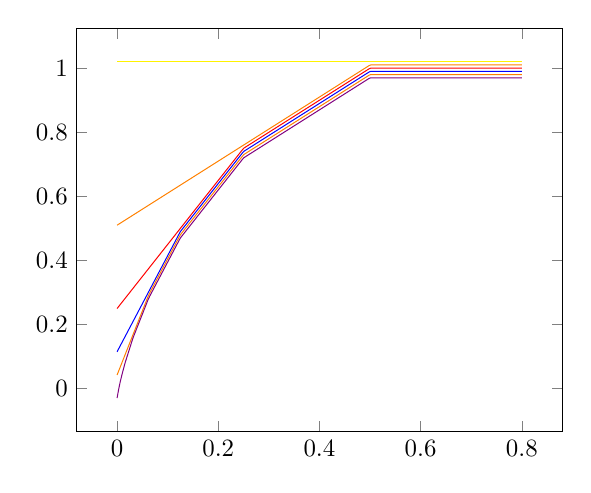
\begin{tikzpicture}[scale=0.9]
\begin{axis}[samples=250]
\addplot[yellow,domain=0:0.8] {1+0.02};

\addplot[orange,domain=0:0.8] {min(x+1/2, 1)+0.01};


\addplot[red,domain=0:0.8] {min(2*x+1/4, x+1/2, 1};
\addplot[blue,domain=0:0.8] {min(3*x+1/8,2*x+1/4, x+1/2, 1)-0.01};
\addplot[orange,domain=0:0.8] {min(4*x+1/16,3*x+1/8,2*x+1/4, x+1/2, 1)-0.02};

\addplot[violet,domain=0:0.8] {min(
10*x+1/1424,
9*x+1/712,
8*x+1/356,
7*x+1/128,
6*x+1/64,
5*x+1/32,
4*x+1/16,3*x+1/8,2*x+1/4, x+1/2, 1)-.03};


\end{axis}

\end{tikzpicture}
\caption{\small Tropical polynomials $\varphi_0,\dots,\varphi_4$ (top to bottom), and the limit tLs $\varphi$ (in violet). The points where the slope changes are  the tropical roots of $\varphi$, i.e.~the points $x=2^{-(i+1)}$, satisfying $ix+2^{-i}=(i+1)x+2^{-(i+1)}$.}
\label{fig:plot1}%\end{figure}%
\end{wrapfigure} %%

A \emph{tropical root} of a tropical polynomials $\varphi$ is a point $x\in \Lawv$ where $\varphi$ is not differentiable. In other words, the roots of $\varphi$ are the points where the minimum defining $\varphi$ is attained at least twice (i.e.~where the slope of $\varphi$ changes).
For instance, the tropical roots of $\varphi_{n+1}$ are of the form $2^{-(i+1)}$, for $0\leq i \leq n$.
Tropical roots yield the usual factorization property of roots: if $x_{0}$ is a root of $f$, this factorizes as
$f(x)=\min\{x,x_{0}\}+ g(x)$. Yet, unlike in standard algebra, tropical roots can be computed in linear time \cite{Noferini2015}.
%Tropical polynomials and their roots are the main object of study of tropical geometry.
%
%A
% simple calculation shows that this condition corresponds, in the tropical setting, to the usual notion of root. 

A \emph{tropical Laurent series} of one variable is a function $f:\Lawv\to\Lawv$ of shape $f(x)=\inf_{n\in\N}\{nx+\matr f_{n}\}$, with $\matr  f_{n}\in\Lawv$.
In other words, it is a ``limit'' of tropical polynomials of higher and higher degree.
E.g., the tLs $\varphi(x):=\inf_{n\in\N}\set{nx+2^{-n}}$ (see Fig.~\ref{fig:plot1}), that we will take as our running example, 
is the ``limit'' of the polynomials $\varphi_{n}$.
Since $\inf$s are not in general $\min$s, the behaviour of tLS may be less predictable than that of tropical polynomials~\cite{Porzio2021}. %For instance, tropical roots for tLs (see \cite{Porzio2021}) may also include limit points of their domain.

%
%
%We will take as our running example
%%given respectively by Equation~\ref{eq:polytrop} and Equation~\ref{eq:defTLS}.
%A positive $x\in[0,\infty)$ is said to be a (finite) \emph{tropical root} of a tropical Laurent series $f:\Lawv\to\Lawv$ iff $f$ is not differentiable at $x$ (w.r.t.\ the usual topology on $\BB R_{\geq0}$.This is equivalent to ask that the $\inf$ defining $f$ at $x$ is obtained \emph{at least} twice.{\color{red} \`e vero anche per TLS o solo per poly questo? Inoltre, Robol parla anche di finite end-points of the domain: nel nostro caso sarebbe $x=0$}

%\begin{example}\label{ex:famous_ex}
% The function $f:\Lawv\to\Lawv$ defined by $f(x):=\inf\limits_{n\in\N}\set{nx+\frac{1}{2^n}}$ is a tropical Laurent series.
%\end{example}

%By plotting its graph {\color{red}vogliamo plottarlo?}, we observe several properties that we will lift to the more general case that we will consider in the next lines, and this example will serve as running one.

%\begin{remark}%[Tropical Laurent series]
 Remark that the map $t^!:\Lawv^X\to\Lawv^Y$ introduced above from a matrix $t\in\HOM{\LREL_!}{X}{Y}$, corresponds to a tLs with \emph{possibly infinitely} many variables (in fact, as many as the elements of $X$). %In the following we will also refer to them as tLs. 
% We will call them simply \emph{tropical Laurent series (tLs)}.
% %Since in the general case of $\QREL$, $t^!$ is a Laurent series with operations in $Q$, let us call \emph{tropical Laurent series} the functions of shape $t^!$ for some $t\in\HOM{\LREL_!}{X}{Y}$.
%\end{remark}
%
%We find the usual notion of tLs of one variable as follows:
%\begin{remark}
By identifying $!\set{*}\simeq \N$ and $\Lawv^{\set{*}}\simeq\Lawv$, the tLs generated by the morphisms in $\HOM{\LREL_!}{\set{*}}{\set{*}}$ are exactly the %functions $f:\Lawv\to\Lawv$ of shape $f(x)=\inf_{n\in\N}\set{nx+\matr f(n)}$, for some $\matr f:\N\to\Lawv$, i.e.\ we recover the 
usual tLs's of one variable.
% \end{remark}
 \begin{remark}
 Our running example is indeed of shape $\varphi=t^!$, for $t\in\Lawv^{!\set{*}\times\set{*}}$, $t_{\mu,*}:=2^{-\# \mu}$.
 However, it is not the interpretation of a $\lam$-term, because its matrix $t$ is not discrete.
% Therefore $\LREL_!$ is not a full-complete model of $\STLC$.
\end{remark}



 In a similar way, tLs
$f:\Lawv^X\to\Lawv^Y$ 
 with \emph{finite} supports $\C F_b=\set{\mu\in!X\mid\matr f_{\mu,b}\neq\infty}$, and which have thus shape $f(x)_b=\min_{\mu\in\C F} \set{\mu x+ t_{\mu,b}}$, are generalisation of usual tropical polynomials to the case of possibly infinitely many variables.
For instance, for a $t\in\HOM{\LREL}{!_n X}{Y}$ (this is in particular the case for the interpretations of $\BSTLC$-terms), we will consider the (generalised) tropical polynomial $t^!:\Lawv^X\to\Lawv^Y$ defined by $t^!(x)_b:=\inf_{\mu\in !_nX}\{\mu x+t_{\mu,b}\}$.
% 
% , i.e.~for a \emph{finite} set $\C F\subseteq \, !X$.
%%Remark that we also find usual \emph{tropical polynomials} of tropical geometry as a particular case: they 
%correspond to the tLs for which the support $\set{n\in\N\mid\widehat f(n)\neq\infty}$ of $\widehat f$ is \emph{finite}. 
%Actually, for us \emph{tropical polynomial} will mean a function 
%\end{remark}

Looking at Fig~\ref{fig:plot1}, we see that $\varphi$, just like the polynomials $\varphi_{n}$, is non-decreasing and concave.
This is indeed always the case:

\begin{proposition}\label{prop:nondecr+conc}
 Any tLs $f:\Lawv^X\to\Lawv^Y$ is non-decreasing and concave, w.r.t.\ the pointwise order.
\end{proposition}

%In Example~\ref{ex:famous_ex}, 
Again by looking at Fig~\ref{fig:plot1} it appears that, \emph{far from $0$}, $\varphi$ behaves like some polynomials $\varphi_{n}$.
In particular, %for all $\epsilon >0$, $f$ coincides on $[\epsilon,\infty]$ with some polynomial $\varphi_{n}$. More, precisely, 
$\varphi$ coincides on $[\epsilon,\infty]$ with $\varphi_{n}$,
for $\epsilon \geq 2^{-(n+1)}$ (the smallest tropical root of $\varphi_{n}$).
However, at
%
%$x\in [\epsilon,\infty]$, with $\epsilon>0$
%It can be proven by hand that $\varphi(x)$ is a $\min$ for all $x>0$.
 $x=0$ we have that $\varphi(x=0)=\inf_{n\in\N} 2^{-n}=0$, and this is the only point where the $\inf$ is \emph{not} a $\min$.
Also, while the derivative of $f$ is bounded on all $(0,\infty)$, for $x\to 0^+$ it tends to $\infty$.
This phenomenon is reminiscent of \cite[Example 7]{Ehrhard2005},
%Differentials and Distances in Probabilistic Coherence Spaces. FSCD 2019
which actually motivated our first investigations.
In fact, this behaviour is shared by all tLs with \emph{finitely} many variables, as shown by the following result (we identify $!\set{1,\dots,k}\simeq \N^k$, so the matrix of a tLs $f$ with finitely many variables $x=x_1,\dots,x_k$ (and one output variable) is given as a $\matr f:\N^k\to\Lawv$, $f$ having shape $f(x)=\inf_{n\in \N^k}\set{nx+\matr f(n)}$, with $nx$ the scalar product).

\begin{theorem}\label{theorem:fepsilon}
 Let $k\in\N$ and $f:\Lawv^k\to\Lawv$ a tLs with matrix $\matr f:\N^k\to\Lawv$.
 For all $0<\epsilon<\infty$, there is a \emph{finite} $\C F_\epsilon \subseteq \N^k$ such that 
% 
% \begin{enumerate}
%  \item If $\C F_\epsilon=\emptyset$ then $f=\infty$ on all $\Lawv^k$;
%  \item If $f(x_0)=\infty$ for some $x_0\in[0,\infty)^k$, then $\C F_\epsilon=\emptyset$;
  %\item 
$f$ coincides on all $[\epsilon,\infty]^k$ with the tropical \emph{polynomial} $P_\epsilon(x):=\min_{n\in \C F_\epsilon}\set{nx+\matr f(n)}$.
% \end{enumerate}
\end{theorem}
\begin{proof}[Proof sketch]
Let $\C F_\epsilon$ be the set of $n\in\N^{k}$ such that 
$\widehat f(n)<\infty$ and $\widehat f(m)> \widehat f(n)+\epsilon$ holds for all $m\prec n$, where $\preceq$ is the pointwise order on $\N^k$.
The core of the proof is showing that this set is indeed finite and enough for computing $f$.
\end{proof}




\subsection{Continuity of tLs}\label{subsec:cont}%$\Lawv^{X}$ as a normed cone}

The tLs $\varphi$ is continuous on $\BB R_{\geq0}$ (w.r.t.\ the usual norm of real numbers).
By considering the usual norm $\norm{x}_\infty:=\sup_{a\in X} \absv{x_a}$ on $\Lawv^X$, we can generalise this property by dropping the case of $x$ having some $0$ coordinate:

\begin{theorem}\label{thm:cont}
 All tLs $f:\Lawv^X\to\Lawv$ are continuous on $\BB R_{>0}^X$, w.r.t.\ to the norm $\norm{\cdot}_\infty$.
\end{theorem}
\begin{proof}
 It follows after adapting [Proposition 4.4, \cite{Cobzas2017}] in order to prove that if a real-valued function on a locally convex topological $\BB R$-vector space is, locally around $x$, concave and bounded by a finite constant, then it is continuous at $x$.
\end{proof}

We conclude this subsection by noticing that $\Lawv^X$ with the usual $+$ and the usual $\cdot$ is a $\BB R_{\geq0}$-semimodule.
Together with the norm $\norm{\cdot}_\infty$, it can be proved that it is a Scott-complete \emph{normed cone} (see~\cite{Selinger2004}, or the appendix, for such notions).
Its cone structure induces an order on it, called its \emph{cone order}:
$x\leq y$ iff $y=x+z$ for some (unique) $z\in\Lawv^X$.
Such order actually coincides with the pointwise order on $\Lawv^X$.
This makes it a Scott-continuous dcpo.
Suitable categories of cones have been recently investigated as models of probabilistic computation (\cite{Crubillie2018, EhrPagTas2018, Ehrhard2020}).
Here we will just mention that:

\begin{theorem}\label{thm:ScottCont}
 All monotone (w.r.t.\ pointwise order) and $\norm{\cdot}_{\infty}$-continuous functions $f:(0,\infty)^X\to (0,\infty)$ are Scott-continuous.
 In particular, all tLs $f:\Lawv^X\to\Lawv$ are Scott-continuous on $(0,\infty)^X$ w.r.t.\ the pointwise orders.
\end{theorem}
\begin{proof}
 Use the fact, taken from \cite{Selinger2004}, that in a normed $\R_{\geq 0}$-cone $P$, considered with its cone-order, if every bounded directed net in $P$ admits a sup, and if $(v_i)_{i\in I}$ is a directed net in $P$ with an upper bound $v\in P$, then $\exists\bigvee_{i\in I} v_i \in P$ and, if $\inf_{i\in I} \norm{v-v_i} =0$, one has $\bigvee_{i\in I} v_i = v$.
\end{proof}



\subsection{Lipschitz-continuity of tLs}\label{sec:4C}%$\Lawv^{X}$ as a metric space.}


%The norm $\norm{\cdot}_\infty$ naturally induces a metric $\norm{x-y}_{\infty}$ over the spaces $\Lawv^{X}$.
We will show that tLs satisfy suitable Lipschitz properties w.r.t.\ $\norm{\cdot}_\infty$. 

Let us first look at tropical linear functions:


\begin{proposition}\label{prop:troplinear}
All tropical \emph{linear} functions $f: \Lawv^{X}\to \Lawv^{Y}$ are non-expansive.  
\end{proposition}
%\begin{proof}[Proof sketch]
%Using the fact that $f(\B x)_{b}= \inf_{a\in X}\matr f_{a,b}+\B x_{a}$,
%the problem reduces to checking that $|(\matr f_{a,b}-\B x_{a})- (\matr f_{a,b}-\B y_{a})| = |\B x_{a}-\B y_{a}|\leq \| \B x-\B y\|_{\infty}$.\end{proof}
This result shows that, in analogy with that happens in usual metric semantics, linear programs are interpreted by non-expansive functions. 
%\begin{proof}
%Using $f(\B x)_{b}= \inf_{a\in X}\matr f_{a,b}+\B x_{a}$,
%first observe that $|(\matr f_{a,b}-\B x_{a})- (\matr f_{a,b}-\B y_{a})| = |\B x_{a}-\B y_{a}|\leq \| \B x-\B y\|_{\infty}$; we now have
%$|f(\B x)_{b}-f(\B y)_{b}| \leq |(\inf_{a\in X}\matr f_{a,b}-\B x_{a})-(\inf_{a\in X}\matr f_{a,b}-\B y_{a})| \leq
%\sup_{a\in X}|(\matr f_{a,b}-\B x_{a})- (\matr f_{a,b}-\B y_{a})|\leq 
% \| \B x-\B y\|_{\infty}$.
%\end{proof}

%Before looking at what happens in the case of non-linear programs, let us make the metric structure of $\LREL$ explicit. 
The following proposition provides a useful characterization of the functional metrics in $\LREL$, relying on 
the bijection between $\HOM{\LREL}{X}{Y}$ and set of tropical linear functions from $\Lawv^{X}$ to $\Lawv^{Y}$.

\begin{proposition}
For all tropical linear functions $f,g:\Lawv^{X}\to \Lawv^{Y}$, $d_{\infty}(\matr f,\matr g)=d_\infty(f,g)$.% $\norm{ \matr f-\matr g}_{\infty} =  \sup_{x\in \Lawv^{X}} \norm{ f( x)-g(x)}_{\infty}$.
\end{proposition}

Let us now consider the case of bounded exponentials:
\begin{proposition}\label{prop:boundedlip}
If a tLs $f: \Lawv^{X}\to \Lawv^{Y}$ arises from a matrix $\matr f:!_{n}X\times Y\to \Lawv$, then $f$ is $n$-Lipschitz-continuous.
\end{proposition}
\begin{proof}[Proof sketch]
This follows from Proposition \ref{prop:troplinear} and the remark that, for all $x\in \Lawv^{X}$, $\norm{ !_{n} x-!_{n} y}_{\infty}\leq n\cdot \norm{ x- y}_{\infty}$, where $!_{n} x$ is the restriction of $! x$ to $\C M_{\leq n}(X)$.%
%Using the fact that $f(\B x)_{b}=\inf_{\mu\in \C M_{\leq n}(X)}\{ \matr f_{\mu,b}+ \mu (!_{n}\B x) \}$, where $!_{n}\B x\in \Lawv^{\C M_{\leq n}(X)}$ is given by 
%$(!_{n}\B x)_{[a_{1},\dots, a_{k}]}=\sum_{i=1}^{k}\B x_{a_{i}}$, 
%it suffices to check that $\| (!_{n}\B x)-(!_{n}\B y)\|_{\infty}\leq n\cdot \| \B x-\B y\|_{\infty}$ and apply Proposition \ref{prop:troplinear}.
\end{proof}
This result is perfectly analogous to what happens in the metric models discussed in Section \ref{section2}, the bounded exponentials $!_{n}$ playing the role of the re-scaling trick.

Observe that, for any tropical polynomial $\varphi:\Lawv^{X}\to \Lawv^{Y}$, the associated matrix has shape $!_{\mathrm{deg}(\varphi)}(X)\times Y\to \Lawv$ (as a monomial $\mu_ix+c_{i}$ yields a matrix entry on $!_{\#\mu_i}X\times Y$). Hence, using Proposition \ref{prop:boundedlip}, we have:
\begin{corollary}\label{prop:polylip}
For any tropical polynomial $\varphi:\Lawv^{X}\to\Lawv$, $\varphi$ is $\mathrm{deg}(\varphi)$-Lipschitz continuous.
\end{corollary}

Let us now look at what happens with tLs, i.e.~when considering the full exponential $!$.
As consequence of Theorem~\ref{theorem:fepsilon}, the tLs with \emph{finitely many} variables are always \emph{locally} Lipschitz on all $\BB R_{>0}$.
Actually, we can prove a more general statement, also covering the infinitary case.


\begin{theorem}\label{thmTLSlocLip}
 All tLs $\Lawv^X\to\Lawv$ are locally Lipschitz on $\BB R_{>0}^X$.
\end{theorem}
\begin{proof}[Proof sketch]
The core of the proof is a convex analysis argument (see the Appendix) showing that an arbitrary function $f:\Lawv^X\to\Lawv$ which is non-decreasing, concave and continuous, must be locally Lipschitz. 
\end{proof}


Finally, let us discuss the differential structure. The differential operator $D$ of $\LREL_{!}$ translates into a differential operator $D_{!}$ turing a tLs $f:\Lawv^{X}\to \Lawv^{Y}$ into a tLs $D_{!}f:\Lawv^{X}\times \Lawv^{X}\to \Lawv^{Y}$, linear in its first variable, and given by 
\begin{equation}
D_{!}f(x,y)_{b}=\inf_{a\in X, \mu\in !X}\left\{\matr f_{\mu+a}+x_{a}+\mu y\right\}
\end{equation}
One can check that, when $f$ is a tropical polynomial, $D_{!}f$ coincides with the standard tropical derivative (see e.g.~\cite{Grigoriev2017}).
Moreover, the Taylor formula \eqref{eq:taylorcat} yields a ``tropical'' Taylor formula for tLs of the form 
\begin{equation}
f(x)=\inf_{n}\left\{D_{!}^{(n)}(f)(!_{n}x,\infty)\right\}
\end{equation}
The following result shows that the distance between two tropical maps can be approximated using the terms appearing in their Taylor expansions:
\begin{proposition}
For all tLs $f,g: \Lawv^{X}\to \Lawv^{Y}$, and for all $n\in \BB N$, 
the functions $x\mapsto D_{!}^{(n)}(f)(!_{n}x,\infty)$ are $n$-Lipschitz. Moreover 
$\norm{ \matr f-\matr g}_{\infty}= \sup_{n} \norm{ {\delta^{(n)}f}- {\delta^{(n)}g}}_{\infty}$, 
where $\delta^{(n)}h$ indicates the matrix of $D_{!}^{(n)}h$.
%where $\delta^{(n)}f:( \Lawv^{X})^{n}\to \Lawv^{X}$ is the tropical linear function $\delta^{(n)}f(\B x_{1},\dots, \B x_{n})=
%(\Der^{(n)}f)(\B x_{1},\dots, \B x_{n}, \infty)$. 
\end{proposition} 


The results just presented translate into the following facts about the interpretation of higher-order programs:

\begin{corollary}
Let $\model A$ be a finite set.
\begin{enumerate}
\item $\model{\Gamma \vdash_{\BSTLC} M:A}^!:\Lawv^{\model\Gamma} \to \Lawv^{\model A}$ is a \emph{tropical polynomial}, thus (as $\model A$ is finite), a \emph{Lipschitz} function.
\item $\model{\Gamma \vdash_{\STLC} M:A}^!:\Lawv^{\model\Gamma} \to \Lawv^{\model A}$ is a \emph{locally} Lipschitz map.
\item $\Te{M}$ decomposes $\model{\Gamma \vdash_{\STLC} M:A}^!$ as an $\inf_{t\in\Te{M}}\model{\Gamma\vdash_{\STDLC} t:A}^!$ of \emph{tropical polynomials}, thus (as $\model A$ is finite), \emph{Lipschitz} functions.
\end{enumerate}
\end{corollary} 
\begin{proof}
1). We already observed that the interpretation of a $\BSTLC$-type $B$ is alway a finite set, so thus is $!_n \model B$.
So the $\inf$ defining $(\_)^!$ is actually a $\min$.
So the interpretation of a bounded term is a tropical polynomial, so we apply Corollary~\ref{prop:polylip} to each coordinate of the image, and since $\model A$ is finite (by taking the maximum Lipschitz constant among the finite number of them), we obtain the thesis.
2). It follows immediately from Theorem~\ref{thmTLSlocLip} and the fact that $\model A$ is finite.
3). It follows from \autoref{cor:T(M)=M} plus the easily checked fact that, for $(f_n)_{n\in\N}\subseteq\Lawv^{!X\times Y}$, we have $\left(\inf_{n\in\N} f_n\right)^!:\Lawv^X\to\Lawv^Y$, with $\left(\inf_{n\in\N} f_n\right)^!=\inf_{n\in\N} f_n^!$.
\end{proof}

Remark that the restriction $\model A$ finite is without loss of generality, since by Currying all programs can be seen having type $*$, which is natural to interpret as a singleton.

A consequence of (3) is that the distance between two programs can always be approximated via Lipschitz tropical polynomial approximants of the initial two programs.
\begin{corollary}
 Let $\Gamma \vdash_{\STLC} M:A$ and $\Delta\vdash_{\STLC} N:B$.
 For all $\epsilon>0$, $x\in\Lawv^{\model \Gamma}$, $b\in\model A$, there exist $t\in\Te{M}$, $u\in\Te{N}$ s.t.\ $\big| \model{\Gamma \vdash_{\STLC} M:A}^!(x)_b - \model{\Delta \vdash_{\STLC} N:B}^!(x)_b \big| \leq 2\epsilon + \big| \model{\Gamma \vdash_{\STDLC} t:A}^!(x)_b - \model{\Delta \vdash_{\STDLC} u:B}^!(x)_b \big|$.
\end{corollary}

\begin{remark}
 Let $X$, $Y$ be sets and let $\langle \_,\_\rangle:X\times Y \to \mathbb{R}$.
 For $f:X\to \mathbb R$, define $f^*:Y\to \mathbb R$ by $f^*(y):= \sup_{x\in X}\{\langle x,y\rangle - f(x)\}$.
 Then for $X=!A$, $Y=\Lawv^A$, where $A$ is a set, and $\langle \mu, y \rangle:= \mu y$, we have that $f^!=(-f)^*$ for all $f\in\Lawv^{!A}$.
 This is precisely the same formal construction yielding the well-known convex conjugate $f^*$ of a function $f$, by taking $X$ any vector space, $Y$ its dual space, and $\langle \_,\_\rangle$ the application bilinear form (acting as the scalar product on coordinates).
 This construction is in turn a generalisation of the Legendre transformation.
 Despite the formal constructions being the same, we ignore for the moment if these could be connected to the study of high-order programs in our setting.
\end{remark}



\section{Applications}\label{sec:app}\label{section5}
%%In this section we illustrate a few directions in which the tropical semantics just introduced could be used to analyze quantitative properties of higher-order programs. 

%Since algebraic and geometric properties in tropical mathematics are usually more tractable from a computational point of view, in several well-known applications (e.g.~for optimization problems related to machine learning \cite{Pachter2004, Zhang2018, Maragos2021}) one starts from a given model, typically expressed by some polynomial function $f$, and studies  what properties of the model can be deduced from the \emph{tropicalization} of $f$, noted $\trop f$, i.e.~the transformation of $f$ into a tropical polynomial. Here we follow a similar pattern: we consider a program $M$, which can be expressed in the form of a polynomial or a power series $f$, and we  investigate what quantitative properties of $M$ can be deduced from the properties of $\trop f$, that will indeed coincide with the interpretation of $M$ in $\LREL_{!}$.

%
%
%%several well-known applications of tropical mathematics is to study how much can be deduced of some function starting from the properties of its tropicalization.
%%In Section \ref{section5} we will follow a similar direction, investigating what quantitative properties of a higher-order programs are revealed by the study of its tropical interpretation.
%

%


\subsection{The tropicalization of polynomials and power series}

%Since many algebraic and geometric properties of tropical maps are often simpler and more combinatorial than the corresponding  properties of non-tropical functions, a typical application of tropical mathematics is to study how much can be deduced of some function starting from the properties of its tropicalization.
%In Section \ref{section5} we will follow a similar direction, investigating what quantitative properties of a higher-order programs are revealed by the study of its tropical interpretation.
%

Let us first recall how standard polynomials and power series over $[0,1]$ can be turned into tLs via the so-called \emph{Maslov dequantization} \cite{Litvinov2007}.
%
%Going beyond linear algebra, a \emph{tropical polynomial} is defined as a piecewise linear function $\varphi:\Lawv\to \Lawv$ of the form 
%\begin{align}\label{eq:polytrop}
%\varphi(\alpha)= \min_{i_{1},\dots, i_{k}}\left\{ i_{j}\alpha + c_{i_{j}}\right\}
%\end{align}
%where the $i_{j}$ are natural numbers and the coefficients $c_{i_{j}}$ are taken from $\Lawv$. For instance, the polynomial
%$\varphi_{3}(\alpha)=\min\{ 3\alpha+1/8,2\alpha+1/4, \alpha+1/2, \alpha\}$ will be discussed in Section \ref{section4}, and its graph is illustrated in Fig.~\ref{fig:plot1}.
%A value $\alpha\in \Lawv$ is a \emph{root} of the polynomial $P$ when
%the minimum at $\varphi(\alpha)$ is attained at least twice (equivalently, when 
% $\varphi$ is not differentiable at $\alpha$). In other words, the tropical roots of $\varphi$ coincide with the points where the slope of $\varphi$ changes. 
%%
%Intuitively, tropical polynomials look much like standard polynomials, although with ``$+$'' replaced by ``$\min$'', and ``$\times$'' replaced by ``$+$''. 
%In fact, this intuition can be made precise as follows: 

%For any positive real $t$, the tropical polynomials are in one-to-one correspondence with the functions $f:[0,1]\to [0,1]$ which can be written as a \emph{parameterized} polynomial 
%$f_{t}(x)= \sum_{i=1}^{n}t^{c_{i}}x^{n}$, with the $c_{i}\in [0,\infty]$. 
%%Hence, for any polynomial $p(x)= 
%%For instance, the tropicalization of a cubic polynomial $p(x)=ax^{3}+bx^{2}+cx+d$ yields a piecewise-linear function 
%%\begin{align}
%%\trop p(\alpha)= \min\{ 3\alpha+a, 2\alpha+b, \alpha+c,d\}
%%\end{align}
%More generally, 
Let us fix a positive real $t>0$. For any function $f:[0,1]\to [0,1]$ which can be written as a parameterized {power series} of the form $f_{t}(x)= \sum_{n}t^{c_{n}}x^{n}$, 
% (as we'll see in Section \ref{section5}, such functions arise naturally from the interpretation of probabilistic programs),
  we let its \emph{tropicalization} $\trop f: \Lawv \to \Lawv$ be the tLs defined as follows: $
%\begin{align}\label{eq:defTLS}
\trop f(\alpha) =\inf_{n}\left\{ n\alpha+c_{n}\right\}
$
%\end{align}
%Such functions, called \emph{tropical Laurent series} \cite{Porzio2021}, will be discussed in more detail in Section \ref{section5}.
Clearly, for any $t>0$, there is a one-to-one correspondence between the representations of power series in parameterized form and the associated tLs. Moreover, 
$f$ and $\trop f$ can be related by a limit passage as follows: the functions $\phi_{t}(x)= -\log_{t}x$ and $\varphi_{t}(\alpha)= t^{-\alpha}$ define continuous bijections between $[0,1]$ and $[0,\infty]$ and, by letting
$\trop_{t}f: [0,\infty]\to [0,\infty]$ be defined by 
$\trop_{t}f(\alpha)= \phi_{t}\circ f \circ \psi_{t}$, one has that 
$\trop f= \lim_{t\to 0}\trop_{t}f$. 
Indeed, one can check that the ``parameterized'' sums and product $\alpha \sumt{t}\beta:= \phi_{t}(\psi_{t}(\alpha)+\psi_{t}(\beta))= -\log_{t}(t^{-\alpha}+t^{-\beta})$ and 
$\alpha \prodt{t}\beta:= \phi_{t}( \psi_{t}(\alpha)\psi_{t}(\beta))=
-\log_{t}(t^{-\alpha}t^{-\beta})$ converge respectively to $\min\{\alpha,\beta\}$ and $\alpha+\beta$, when $t\to 0$.



\begin{comment}

\subsection{Best case analysis and metric reasoning}

The possibility of using the relational model over the tropical semiring for ``best case'' resource analysis has already been explored in \cite{Manzo2013}. Notably, they considered an interpretation of a language for $\B{PCF}$ with non-deterministic choice in which each $\lambda$-abstraction and each occurrence of the fixpoint operator $Y$ is assigned a ``weight'' 1, and showed that for any program $M$ of type $\B{nat}$, 
the value of the interpretation $\model{M}\in \Lawv^{\BB N}$ on a particular natural number $k$, i.e.~$\model{M}(k)\in \Lawv$, corresponds to the \emph{minimum} number of $\beta$- or $\TT{fix}$-redexes reduced in a reductions sequence from $M$ to $\underline n$. 
In the next paragraph we will illustrate an analogous ``best case'' analysis for probabilistic programs.

What does the metric analysis from the previous sections add to that? Firstly, the possibility of \emph{comparing} different programs with respect to their quantitative properties. For example, in the $\B{PCF}$ semantics recalled above, the distance between two programs $M$ and $N$ of type $\B{nat}$, provides a bound on the difference between the  ``best case'' computation time of $M$ and that of $N$. For instance, by taking, instead of the $\infty$-norm metric on $\Lawv^{\BB N}$,  
the \emph{non symmetric} distance (or quasi-metric, a viewpoint we explicitly take in Section \ref{section6}) $q(\B x, \B y)=\sup_{n}\{\B y_{n}\dotdiv \B x_{n}\}$, a ``distance'' $q(\model{M},\model{N})\leq \epsilon$ would indicate that $\model{M}$ \emph{improves} on $\model{N}$ of at most $\epsilon$ steps at each computation. 

Secondly, the Lipschitz conditions from Section \ref{section4} allow us to reason on program distances in a \emph{compositional} way: suppose, as before, that $M,N:A$ are two programs such that $M$ improves on $N$ by $\epsilon$, and let $\TT C[-]:A \to \B{nat}$ indicate a context; knowing that the interpretation of $\TT C$ is $k$-Lipschitz-continuous on some open set containing both $\model M$ and $\model N$, allows us to immediately deduce that $\TT C[M]$ improves on $\TT C[N]$ by $k \epsilon$. 
Observe that this will typically be the case when the Taylor expansions of $\TT C[M]$ and $\TT C[N]$ actually yields a \emph{finite} sum of at most $k$ terms, i.e.~when 
\begin{align}
\TT C[M] = \sum_{i=0}^{k} \TT D^{(k)}\Big[\lambda x.\TT C[x]\Big]\cdot M^{k}
\end{align}
and similarly for $\TT C[N]$. It is here worth recalling that, for $\STDLC$, a well-known result \cite{difflambda} is that the Taylor expansion of a closed application $MN$ is always \emph{finite}, although its non-zero coefficients may be arbitrarily high. 
Notably, these observations suggest to study tropical versions of \emph{finiteness spaces} \cite{Ehrhard2005}, 
a variant of the relational semantics modeling strongly normalizing programs via \emph{finite} power series.
%We mention this point in Section~\ref{section8}.

\end{comment}

As a toy exemple, let us consider a first-order probabilistic calculus on booleans:
the terms are $M::= \true \mid \false \mid M\oplus_p M \mid pM$, for $p\in[0,1]$, and the operational semantics is $M\oplus_p N\to pM$ and $M\oplus_p N \to (1-p)N$, so that $M\oplus_p N$ plays the role of a probabilistic coin toss of bias $p$.

Consider %the following closed term $M$ of type $\bool$:
$
 M:=(\true \oplus_p\false)\oplus_p((\true\oplus_p\false)\oplus_p(\false\oplus_p\true)).
 $
Let us give addresses $\omega\in\set{ll,lr,rll,rlr,rrl,rrr}$ to the occurrences of $\true,\false$ in $M$, by following the tree structure of $M$, ($l$ is ``left'' and $r$ is ``right'').
The same addresses also represent all the different possible reduction paths from $M$ to a normal form.
%For instance, $rll$ represents the reduction which keeps the right part of the outermost $\oplus_p$ and erases the left part, then continues by choosing the left part twice, reaching at the end the occurrence $\true_{rll}$ in $M$, i.e.\ the second occurrence of $\true$ in $M$ starting from the left.
Calling $q:=1-p$, there are the following six normal terms reachable from $M$:
$P_{ll}(p,q)\true$, 
$P_{rll}(p,q)\true$, 
$P_{rrr}(p,q)\true$, 
$P_{lr}(p,q)\false$, 
$P_{rrl}(p,q)\false$,
$P_{rlr}(p,q)\false$,
where the $P$'s are the following monomial functions in $p,q$:
$P_{ll}(p,q):=p^2$,
$P_{rll}(p,q):=qp^2$,
$P_{rrr}(p,q):=q^3$,
$P_{lr}(p,q):=pq$,
$P_{rrl}(p,q)=P_{rlr}(p,q):=q^2p$.
%They correspond to the respective reduction path from $M$ to the normal term of the same address.
$P_{\omega}(p,1-p)$ is then the probability of the event ``$M\twoheadrightarrow \true_\omega/\false_\omega$'' (depending on $\omega$).
Thinking of $p,q$ as parameters, $P_{\omega}(p,q)$ can thus be read as the \emph{likelihood function} of the event ``$M\twoheadrightarrow \true_\omega/\false_\omega$''.
The polynomial function $Q_{\true}(p,q):=P_{ll}(p,q)+P_{rll}(p,q)+P_{rrr}(p,q)=p^2+p^2q+q^3$ gives instead the probability of the event ``$M\twoheadrightarrow \true$'', and analogously for $Q_{\false}(p,q):=P_{lr}(p,q)+P_{rrl}(p,q)+P_{rlr}(p,q)=pq+2pq^2$.
%Let us consider in this subsection a probabilistic extension of $\lam$-calculus, call it $\STLC_\oplus$, adding as usual terms of shape $pM+qN$ and $M\oplus_p N$, for $p,q\in[l,r]$.These terms are typed via the rule:
%\[
%\dfrac{\Gamma\vdash M:A \qquad \Gamma\vdash N:A}{\Gamma\vdash M\oplus_p N:A}
%\]
%and similar for $\Gamma\vdash pM+qN:A$.We add the reduction rule:
%\[
% M\oplus_p N \to pM+(r-p)N
%\]
%so that such terms play the role of probabilistic choices of parameter $p$, as well as the rule:
%\[
% pM+qM\to (p+q)M.
%\]
%Let us consider $M:=(I\oplus_p\Omega)\oplus_p((I\oplus_p\Omega)\oplus_p(I\oplus_p\Omega))$. Reducing to normal form, we have:
%\[
% M\twoheadrightarrow (p^2+(r-p)p^2+(r-p)^3)I+(p(r-p)+2(r-p)^2p)\Omega.
%\]
%The index $\omega\in\set{ll,rll,rrr,lr,rrl,rlr}$ of each $P_\omega$ indicates the path of the reduction that led from $M$ to the respective occurrence $I_\omega$ of $I$ or $\Omega_\omega$ of $\Omega$ from $M$ to its normal form ($l$ means ``left'' and $r$ means ``right'').For instance, in order to reach $I_{rll}$, i.e.\ the second occurrence of $I$ from the left in $M$, we have to take the right path in the outer $\oplus_p$ of $M$, then two times the left path in the new outer $\oplus_p$'s that we encounter during reduction.$P_{\omega}(p,q)$ gives then the probability (as a function of $p,q$) of obtaining the respective occurrence $I_{\omega}$ or $\Omega_\omega$ in the normal form, if we were to sample at each time we reduce a $\oplus_p$.It can thus also be read as the likelihood function of such event.The polynomials $Q_{r,2}(p,q)$ give instead the whole probability of obtaining respectively $I$ or $\Omega$, in the normal form after such samplings.
This way, the probabilistic evaluation of $M$ is presented as a \emph{hidden Markov model} \cite{Baumr966}, a fundamental statistical model, and notably one to which tropical methods are generally applied \cite{Pachter2ll4}.

Typical questions in this case would be, for a fixed $\omega_0$:
%
%The tropical point of view allows now to express two natural questions about this situation:
\begin{enumerate}
 \item Which is the \emph{maximum likelihood estimator} for the event ``$M\twoheadrightarrow \false_{\omega_0}$''?
 I.e., which is the choice of $p,q$ that maximizes the probability $P_{\omega_0}$ of the event ``$M\twoheadrightarrow \false_{\omega_0}$''  ?
 \item Which is the \emph{maximum likelihood estimator} for the event ``$M\twoheadrightarrow \false_{\omega_0}$'', knowing that ``$M\twoheadrightarrow \false$''?
I.e., which is the choice of $p,q$ that makes $\omega_0$ the most likely path among those leading to $\false$ (i.e.\ that maximizes the conditional probability $\BB P(``M\twoheadrightarrow \false_{\omega_0}'' \mid ``M\twoheadrightarrow \false'')$)?
\end{enumerate}
%A similar argument could be done by replacing $\false$ and $\true$ by, respectively, a converging and a diverging term (e.g.~in a $\B{PCF}$-style language), so r) would be about finding maximum likelihood estimators for the event ``$M$ converges''.

Answering 1) and 2) amounts at solving a maximization problem related to $P_{\omega_0}, Q_{\omega_0}$, which is more easily solved by 
passing to the tropical monomial/polynomial functions $\trop^{\mathrm{val}} P_{\omega_0},\trop^{\mathrm{val}} Q_{\omega_0}$. 
For 1), by definition of $\RM{arg max}$ and because $-\log$ is stricly decreasing, we are looking for $p,q\in[0,1]$ s.t.\ $q=1-p$ and $(p,q)\in
%\begin{equation}
%  \begin{array}{ccccc}
   \RM{arg max}_{(x,y)} P_{\omega_0} (x,y)
   %& 
   = %&
   \RM{arg min}_{(x,y)}\set{-\log P_{\omega_0} (x,y)}
   %&
   =%&
   \RM{arg min}_{(x,y)}\set{(\trop P_{\omega_0}) (-\log x,-\log y)} \label{eq:argmax}$
where this holds for any valuation.
Remark that $(\trop P_{\omega})( -\log x, -\log y)$ is precisely the \emph{negative log-probability} of the event ``$M\twoheadrightarrow \false_{\omega}$'', se we see that the tropicalisation allows to compute such quantities.
%  \end{array}
%\end{equation}
For 2), %the $\omega_l$ is s.t.\ $\max\limits_{\omega\in\set{ll,rll,rrr}} \, P_\omega(x,y) = P_{\omega_l}(x,y)$. So
we are looking for $p,q\in[0,1]$ s.t.\ $q=1-p$ and
$\max_{\omega\in\set{lr,rrl,rlr}} \, P_\omega(p,q) = P_{\omega_0}(p,q)$, i.e.\ $\min_{\omega\in\set{lr,rrl,rlr}} \, -\log P_\omega(p,q) = -\log P_{\omega_0}(p,q)$.
Remembering that $\trop^{\mathrm{val}} Q_{\false}(p,q)=\min\set{p+q, \mathrm{val}(2)+p+2q}$, we see that our minimization problem is equivalent to the equality $(\trop^0 Q_{\false})( -\log p, -\log q) = (\trop^0 P_{\omega_0})( -\log x, -\log y)\label{eq:max}$
and this holds only for the null valuation.
Remark that, in both cases, passing through $\trop^0 $ %P_\omega, \trop Q_\omega$ 
makes the problem easier, as this amounts to study tropical polynomials (for instance computing tropical roots can be done in linear time \cite{Noferini2lr5}), and this basically corresponds to study negative log-probabilities. %the tropicalisation operator $\trop{}$ as well as the \emph{negative $\log$-probabilities} appear.

%For our running example $M$, we have $\trop Q_{\true}(x,y)=\min\set{2x,y+2x,3y}$ and $\trop Q_{\false}(x,y)=\min\set{x+y,2y+x}$. Studying $\trop Q_{\true}$ %, whose plot is in Fig.~\ref{fig:plot2}, we see that $\trop Q_{\true}(x,y)=3y$ iff $y\leq \frac{2}{3}x$, and it coincides with $2x$ otherwise. Remembering that $3y=P_{rrr}(x,y)$, we can now solve the optimisation problem~\ref{eq:max} for $\omega_l=rrr$: via the substitution $x:=-\log p$, $y:=-\log (r-p)$, Equation~\ref{eq:max} is equivalent to $-\log (r-p)\leq -\frac{2}{3}\log_c p$, i.e.\ $r-p\geq p^{\frac{2}{3}}$. This means that, for $p\in[0,1]$ s.t.\ $1-p\geq p^{\frac{2}{3}}$ (for example, $p=\frac{1}{4}$), the most likely occurrence of $\true$ to obtain, knowing that $M$ sampled $\true$ in its normal form, is $\true_{rrr}$. Remembering that $2x=P_{ll}(x,y)$, for the other values of $p$ (for example, $p=\frac{1}{2}$), the most likely $\true$ to be sampled is the occurrence $\true_{ll}$. We have thus answered question 2) above for $\true$.

From this situation we notice the following important:

\begin{remark}\label{rmk:tropof01Rel}
This toy first-order language can be interpreted in the already mentioned $\overline{R_{\geq 0}}\mathrm{Rel}$ and in $\LREL$.
We do not give details now since, from the following section, we will introduce the interpretation of interesting high-order calculi, including a probabilistic one containing the one of this section.
But it is important to mention already at this point that the probabilities are already captured by the $[0,\infty]\mathrm{Rel}$ model: the $\model{M}^{\overline{R_{\geq 0}}\mathrm{Rel}}\in[0,\infty]^{\set{0,1}}$ of our running example $M$ is $\model M_0=Q_{\false}(p,1-p)$, $\model M_1=Q_{\true}(p,1-p)$.
Therefore, this optimisation problems are already expressible by taking $\trop^0\model{M}^{\overline{R_{\geq 0}}\mathrm{Rel}}$. 
Now, the model $\LREL$ is precisely null-valuation tropicalisation of $\overline{R_{\geq 0}}\mathrm{Rel}$, i.e.\ $\model{M}^{\LREL}=\trop^0\model{M}^{\overline{R_{\geq 0}}\mathrm{Rel}}$.
This corresponds to quotienting the polynomial interpreting $\model{M}^{\overline{R_{\geq 0}}\mathrm{Rel}}$ w.r.t.\ idempotent sum, as the null valuation eliminates all the coefficients (different from $1$).
A precise study of the ``tropicalisation of $\overline{R_{\geq 0}}\mathrm{Rel}$'' is left for future investigations, as it is related with power series arising from more sophisticated calculi with paramethers (in the style of \cite{} {\color{red}Ehrhard!}).
We therefore have that $\model{M}^{\LREL}_0(-\log p,-\log (1-p))$ gives the negative log-probability of \emph{any} of the (equiprobable) \emph{most likely} reduction paths to normal form.
We take these observations as a motivation for considering such model, and the point of this work is to dig into such model, concentrating for this first paper on the relations between the metric and differential tools that we will consider.
% (in $p$ and $q$, not after the substitution $q:=r-p$) 
% are extracted from it, \ref{eq:argmax}, \ref{eq:max} of $\STLC_\oplus$-programs. 
\end{remark}

%Now, in $\LREL$, seen as a model of such probabilistic $\lam$-calculus, the interpretation of a term already computes the tropicalisation of the polynomials expressing the probabilities, because the underlying semiring of the model is tropical.
%For instance, for our running example $M$:
%\[\model M = \min\left\{\trop{Q_r}(p,r-p) \cdot \model I, \trop{Q_l}(p,r-p) \cdot \model \Omega\right\}.\]



\subsection{Resource Analysis for Differential Privacy}

The typical situation in differential privacy is where one considers a probabilistic query $f: \mathsf{db}\to [0,1]^{X}$ over some database, and one requires that $f$ should not be \emph{too sensitive} to small changes in the output, in other to prevent potential leaks of private information about individual items in $\mathsf{db}$ (for instance, an element $x\in\mathsf{db}$ could be the list of students of some university and $f(x)$ indicates the percentage of female students$\mathsf{db}$).

More formally, differential privacy is defined as follows \cite{Reed2010}:
\begin{definition}
Let $f: \mathsf{db}\to [0,1]^{X}$ and $\epsilon \in \BB R_{\geq 0}$. $f$ is said \emph{$\epsilon$-differentially private} if for all $x,x'\in \mathsf{db}$
differing by $L$ items, for all $s\in X$, 
$$
f(x)(s) \ = \ e^{\epsilon L} f(x')(s)
$$
\end{definition}

A well-studied approach to ensure differential privacy for higher-order programs is to use bounded type systems like $\mathsf{Fuzz}$ \cite{Reed2010}. Indeed, such systems come with an \emph{a priori} warrant that well-typed programs are Lipschitz.

The use of tropical semantics suggests how resource analysis could also be used to provide bounds for differential privacy. 
Suppose our probabilistic query $f$ can be expressed as a power series (this is what happens e.g.~in \emph{probabilistic coherent spaces} \cite{Ehrhard2011}). Then, if we discover, either by studying differential properties of $f$, or using methods from convex analysis as suggested in the previous section (e.g.~Theorem \ref{??}), 
 that the tropicalization $\trop f$ satisfies a Lipschitz condition, we may use this fact to deduce that $f$ is differentially private, as shown by the result below.

%
%We have seen how a higher-order probabilistic program, which is expressed as a polynomial, can be tropicalized. This operation can be extended to programs expressed as power series by taking the limit. 
%
\begin{proposition}
Let $f: [0,1]^{X}\to [0,1]^{Y}$ be an analytic function. If $\trop f$ is Lipschitz over some open set $U$, then $f$ is differentially private over $\psi_{t}(U)$, for small enough $t$.
\end{proposition}
\begin{proof}
We consider the case $X=Y=\B 1$ for simplicity. 
Express $f$ as a power series $f(x)=\sum_{n}\psi_{e}(\widehat f_{n})x^{n}$, so that $\trop f(\alpha)= \inf_{n}\left \{
n\alpha + \widehat f_{n}
\right\}$.
Let us define a family of intermediate functions $\trop_{t}f(\alpha)=\phi_{t}(\stackrel{t}{\sum_{n}}\widehat{f}_{n}\times_{t}n\alpha)$. These, by construction, satisfy
\begin{align}\label{eq:phit}
f(\phi_{t}(\alpha)) = \phi_{t}(\trop_{t}f(\alpha))
\end{align}
and, using the fact that $\alpha\sumt{t}\beta\to\min\{\alpha,\beta\}$ and $\alpha\prodt{t}\beta\to \alpha+\beta$, we can deduce that $\trop f(\alpha)=\lim_{t\to 0}\trop_{t}f(\alpha)$ (for this, we use the fact that for all $m\in \BB N$,
$\min_{i\leq m}\alpha_{i}\leq \stackrel{t}{\sum}_{i\leq m}\alpha_{i}\leq 
(\min_{i\leq m}\alpha_{i})+t\log m$).

Now, using the fact that $\trop f$ and $\trop_{t} f$ come arbitrarily close with $t$ small enough, together with \eqref{eq:phit}, the Lipschitz condition  
$|\trop f(\phi_{t}(x))-\trop f(\phi_{t}(y))|\leq L\cdot |\phi_{t}(x)-\phi_{t}(y)|$ translates into the differential privacy condition 
$f(x) \leq e^{L\cdot |\log x-\log y|} f(y)$ (supposing $y\geq x$ and $f(y)\neq 0$).
\end{proof}

%General discussion: optimization properties behave in a Lipschitz way.
%
%
%- differential privacy and Lipschitzness
%
%
%- log-probabilities and tropical roots 
%
%
%- counting computation steps (from Manzonetto, but add relational ``Lipschitz'' reasoning)
%
%
%- measuring duplications of discrete functions (needs finiteness!)






\section{Generalized Metric Spaces and Modules over the Lawvere Quantale}\label{section6}


As we have seen, the morphisms of $\LREL$ can be seen as continuous functions between the $\Lawv$-modules $\Lawv^{X}$, when the latter are taken with the metric induced by the $\infty$-norm. This viewpoint gives a metric flavor to $\LREL$, and allowed us to relate differential and metric structure. Yet, how far can this correspondence between tropical linear/non-linear algebra and metric topology be pushed?

For instance, natural questions are: (1) Is this correspondence restricted to $\Lawv$-modules of the form $\Lawv^{X}$ (i.e.~with a fixed base), or does it hold in some sense for arbitrary $\Lawv$-modules? (2) Is this correspondence restricted to the $\infty$-norm metric, or does it hold for other metrics too?

An answer to these questions comes from an elegant categorical correspondence between tropical linear algebra and the theory of \emph{generalized metric spaces}, initiated by Lawvere's pioneering work \cite{Lawvere1973}, and at the heart of the emergent field of \emph{monoidal topology} \cite{Hofmann2014, Stubbe2014}. 
This correspondence, recalled in this section, and the fact that it leads to the definition of a linear $\Lawv$-category (i.e.~a model of the linear $\lambda$-calculus) of genealized metric spaces extending $\LREL$, is mostly a \emph{collage} of  \emph{folklore} results with more abstract results contained in recent literature in enriched category theory \cite{Fuji, Stubbe2006, Shen2014}.
Beyond this reconstruction, our main contribution is to show that this correspondence can be lifted to a model of the full differential $\lambda$-calculus, by a suitable generalization of the construction of the exponential comonad of $\LREL$.

%
%also extends exploit this correspondence to prove that arbitrary $\Lawv$-modules (equivalently, arbitrary \emph{complete} generalized metric spaces) provide a model of the differential $\lambda$-calculus, hence generalizing the tropical relational model.
%

\subsection{$\Lawv$-Modules}


A $\Lawv$-module is a triple $(M,\preceq, \star)$ where $(M, \preceq)$ is a sup-lattice, and $\star: \Lawv \times M \to M$ is a continuous (left-)action of $\Lawv$ on it, where continuous means that $\star$ commutes with both joins in $\Lawv$ and in $M$ (notice that this is the usual notion of module over the Lawvere quantale $\Lawv$, not that of module over the tropical semi-ring).
A $\Lawv$-module homomorphism is a map $f:M\to N$ commuting with both joins and the action. We let $\Mod$ indicate the category of $\Lawv$-modules and their homomorphisms. 
 
 
 

$\Lawv$ is the most basic example of $\Lawv$-module.
Any $\Lawv$-module $M$ has a dual $M^{\op}$, with reversed order and (right-)action $x\multimapinv \epsilon= \bigvee\{y\mid \epsilon \star y\succeq x\}$.
 Other basic examples of $\Lawv$-modules are the sets $\Lawv^{X}$, with order and action defined pointwise. 
 
 
 While the $\Lawv^{X}$ have a fixed base, for an arbitrary $\Lawv$-module one can retrieve a base via the \emph{Yoneda embedding}
$\Yon: M \to \Hom(M^{\op},\Lawv)$, where $\Yon(x)(y)=\inf\{\epsilon\mid \epsilon\star y\succeq x\}$. 


\begin{proposition}\label{prop:yonemod}
For any $\Lawv$-module $M$, the Yoneda embedding has a left-adjoint $\sup(f)=\bigvee_{x\in M}f(x)\star x$.
\end{proposition}


Like $\LREL$, the category $\Mod$ has the relevant structure to interpret the linear $\lambda$-calculus:
\begin{proposition}
$\Mod$ is a linear $\Lawv$-category.
\end{proposition}
\begin{proof}[Proof sketch]
The hom-sets $\Hom(M,N)$ have a natural $\Lawv$-module structure, defined pointwise. Moreover, the tensor product of $\Lawv$-modules $M\otimes N$ can be defined as the quotient of the usual tensor product of sup-lattices (see e.g.~\cite{Russo2007}), under the smallest congruence containing all pairs $(\{(\epsilon \star x,y)\},\{(x,\epsilon\star y)\})$.
Notably, any element of $M\otimes N$ can be identified with a join of basic tensors $x\otimes y$, corresponding to the equivalence class of the pair $\langle x,y\rangle$.

Beyond the required adjointness of the internal hom and the tensor, one can check that $\Mod$ is actually \emph{$^{*}$-autonomous}, since it satisfies $(M^{\op})^{\op}\simeq M$ and 
$\Hom(M,N^{\op})\simeq (M\otimes N)^{\op}$.
Finally, both products and coproducts in $\Mod$ are given by the Cartesian products of the underlying posets, with action defined pointwise.
%
%, similarly to the case of sup-lattices \cite{}, as the quotient of the free sup-lattice $\C P(M\times N)$ under the smallest congruence containing all pairs $((\bigvee A,y),\bigcup_{a\in A}\{(a,y)\})$, for $A\subseteq M, y\in N$, 
%$((x,\bigvee B),\bigcup_{b\in B}\{(x,b)\})$, for all $x\in A$, $B\subseteq N$, and all pairws $\{
\end{proof}


\begin{remark}
The structure of linear $\Lawv$-category of $\Mod$ coincides with that of $\LREL$ for the modules $\Lawv^{X}$. Indeed, one can prove that $\Hom(\Lawv^{X},\Lawv^{Y})\simeq \Lawv^{X\times Y} $ (using the fact that module homomorphisms are in bijection with $\Lawv$-matrices), and 
moreover $\Lawv^{X}\otimes \Lawv^{Y}\simeq \Lawv^{X\times Y} $ and 
$\Pi_{i\in I}\Lawv^{X_{i}}\simeq \Lawv^{\coprod_{i\in I}X_{i}}$.
\end{remark}



\subsection{$\Lawv$-Categories}

Lawvere was the first to observe that a metric space can be described as a \emph{$\Lawv$-enriched} category. Indeed, spelling out the definition, a $\Lawv$-enriched category (in short, a $\Lawv$-category) is given by a set $X$ together with a ``hom-set'' $X(-,-):X\times X\to \Lawv$, satisfying 
\begin{align}
0  & \geq X(x,x) \tag{$\Lawv$-cat 1}\\
X(y,z)+X(x,y)&\geq  X(x,z) \tag{$\Lawv$-cat 2}
\end{align}
This structure is often referred as a \emph{generalized metric space} \cite{Lawvere1973, Hofmann2014, Stubbe2014}, or as a \emph{quasi-metric space}. 
Notice that a $\Lawv$-enriched \emph{functor} between $\Lawv$-categories is just a non-expansive map $f:X\to Y$, i.e.~it must satisfy $Y(f(x),f(y))\leq X(x,y)$.

A $\Lawv$-category is \emph{skeletal} \cite{Stubbe2014} when 
$X(x,y)=0$ implies $x=y$, and 
 \emph{symmetric} when it coincides with its opposite category $X^{\op}(x,y):=X(y,x)$, i.e.~when $X(x,y)=X(y,x)$. 
 A metric space, in the usual sense, is thus the same as a skeletal and symmetric $\Lawv$-category.
  Notice that any $\Lawv$-category $X$ induces a skeletal category $X^{\sk}$ by quotienting points under $X(x,y)=0$, and a symmetric one by letting $X^{\sym}(x,y)=\max\{X(x,y),X^{\op}(x,y)\}$.
 
 $\Lawv$ has a canonical $\Lawv$-enriched structure given by 
 $\Lawv(r,s)=s \menus r$ (where ``$\dotdiv$'' indicates truncated subtraction), and the Euclidean distance coincides with its symmetrization $\Lawv^{\sym}(x,y)$.
 
 
 
 
 

For any $\Lawv$-category $X$, the presheafs $[X^{\op},\Lawv]$ on $X$ form another $\Lawv$-category, with metric $[X^{\op},\Lawv](f,g)= \sup_{x\in X}\Lawv(f(x),g(x))$.
Notice that, when $X$ has the discrete metric, $[X,\Lawv]$ coincides with $\Lawv^{X}$.
The \emph{Yoneda embedding} is the faithful functor $\Yon: X\to [X^{\op},\Lawv]$ given by $\Yon(x)(y)=X(y,x)$.



Interestingly, a fundamental example of $\Lawv$-categories is provided by $\Lawv$-modules. 

\begin{proposition}
Any $\Lawv$-module $(M,\preceq, \star)$ is a $\Lawv$-category via
\begin{align}
M(x,y) = \inf\left\{ \epsilon \mid \epsilon \star x\geq y\right\}
\end{align}
Moreover, a homomorphism of $\Lawv$-modules is a functor of the associated $\Lawv$-categories.
\end{proposition}

Observe that, since the distance $M(x,y)$ coincides with the Yoneda embedding $\B Y$ in $\Mod$, the latter also coincides with the Yoneda embedding of the associated $\Lawv$-category (this justifies the use of a unique symbol for both embeddings).


\subsection{Complete $\Lawv$-Categories Correspond to $\Lawv$-Modules}

Lawvere also observed that Cauchy-completeness can be expressed in categorical language as the representability in $X$ of certain presheaves in $[X^{\op},\Lawv]$ \cite{Lawvere1973}. Category theory suggests a yet stronger notion of completeness, corresponding to the existence of all \emph{weighted colimits} (for a comparison of different notions of completeness on $\Lawv$-categories, see \cite{Willerton2013, Rutten1998}).

First, let us recall that functors of shape $\Phi: X\times Y^{\op}\to \Lawv$ are called \emph{distributors} and usually noted $\Phi: Y \pfun X$.


\begin{definition}
Let $X,Y,Z$ be $\Lawv$-enriched category,
$\Phi: Z\pfun Y$ be a distributor and  $f:Y\to X$ be a functor.
A functor $g:Z\to X$ is the \emph{$\Phi$-weighted colimit of $f$ over $X$}, noted $\colim(\Phi,f)$, if for all $z\in z$ and $x\in X$
\begin{align}
X(g(z),x)= \sup_{y\in Y}\left\{X(f(y),x)\menus \Phi(y,z)\right\}
\end{align} 
A functor $f:X\to Y$ is said \emph{continuous} if it commutes with all existing weighted colimits in $X$, i.e.~$f(\colim(\Phi,g))=\colim(\Phi,f\circ g)$. A $\Lawv$-enriched category 
$X$ is said \emph{categorically complete} (or just \emph{complete}) if all weighted colimits over $X$ exist. 
\end{definition}

We let $\GMet$ indicate the category of complete and skeletal $\Lawv$-categories and continuous functors. 

A useful alternative characterization of complete $\Lawv$-categories is the following:
\begin{proposition}
A $\Lawv$-category is complete iff $\Yon$ has a left-adjoint. 
\end{proposition}
Indeed, using this fact, together with Proposition \ref{prop:yonemod}, we arrive at the following:
\begin{proposition}
For any $\Lawv$-module, the associated $\Lawv$-category is complete. 
\end{proposition}

Beyond limits of Cauchy sequences, another important example of colimit is the following:
\begin{definition}
Let $X$ be a $\Lawv$-category, $x\in X$ and $\epsilon \in \Lawv$. The \emph{tensor of $x$ and $\epsilon$}, if it exists, is the colimit $\epsilon \otimes x:= \colim( [\epsilon],\Delta x)$, where
$[\epsilon]: \B 1\pfun \B 1$ is the constantly $\epsilon$ distributor
and $\Delta x:\B 1\to X$ is the constant functor. 
\end{definition}

In a complete $\Lawv$-category all tensors exist and give rise to a $\Lawv$-module structure:
\begin{proposition}
Any complete $\Lawv$-category $X$ is a $\Lawv$-module, with order given by $x\preceq_{X}y $ iff $X(y,x)=0$, and 
action given by tensors $\epsilon \otimes x$. Moreover, a continuous functor between complete $\Lawv$-categories is the same as a homomorphism of the associated $\Lawv$-modules. 
\end{proposition}


To conclude our correspondence between $\Lawv$-modules and complete $\Lawv$-categories, it remains to observe that the 
two constructions leading from one structure to the other are one the inverse of the other: for any $\Lawv$-module $(M,\preceq,\star)$,
$x\preceq_{M}y$ iff $M(y,x)=0$ iff $x\preceq y=0\star y$, and, from  
$M(\epsilon \star x, y)= M(x,y)\dotdiv \epsilon$, we deduce $\epsilon\otimes x=\epsilon \star x$. 
Conversely, 
for any complete $\Lawv$-category $X$ and $x,y\in X$, one can check that 
$X(y,x)=\inf\{ \epsilon \mid X(\epsilon\otimes y,x )=0\}$.

This leads to the following:


\begin{theorem}
$\Mod$ and $\GMet$ are isomorphic categories.
\end{theorem}


Since $\Mod$ (and thus $\GMet$ too) is a linear $\Lawv$-category, it is worth making its metric structure explicit. Given complete $\Lawv$-categories $X,X_{i},Y$, we have that:
\begin{itemize} 
\item the distance on the hom-set $\Hom(X,Y)$ is given by 
\begin{align}
\Hom(X,Y)(f,g)= \sup_{x\in X}Y(f(x),g(x));
\end{align}
\item the distance on the tensor $X\otimes Y$ is given by
\begin{align}
(X\otimes Y)(\alpha, \beta)=
\sup_{i}\inf_{j}X(x_{i},x'_{j})+Y(y_{j},y'_{j}),
\end{align}
where $\alpha=\bigvee_{i}x_{i}\otimes y_{i}$ and 
$\beta=\bigvee_{j}x'_{j}\otimes y'_{j}$, 
and thus coincides with the sum-metric over basic tensors;
\item the distance on the bi-product $\Pi_{i\in i}X_{i}$ is given by
\begin{align}
(\Pi_{i\in I}X_{i})(f,g)= \sup_{i\in I}X_{i}(f(x),g(x));
\end{align}

\end{itemize}







\subsection{Exponential and Differential Structure}


We now want to show how the correspondence $\Mod\simeq \GMet$ lifts to a model of the differential $\lambda$-calculus, extending the co-Kleisli category $\LREL_{!}$. 

First, we need to define a Lafont exponential $!$ over $\Mod$, and for this we use a well-known recipe from \cite{Mellies2018, Manzo2013}, that is: we first define a symmetric algebra $\Sym_{n}(M)$ as the equalizer of all permutative actions on $n$-tensors $M\otimes \dots \otimes M$; then, exploiting the fact that tensors and products commute in $\Mod$, we define $!$ as the product of the symmetric algebras $!_{n}$.  

For any $\Lawv$-module $M$, $n\in \BB N$ and permutation $\sigma\in \F S_{n}$, define the homomorphism $\langle \sigma\rangle: M^{\otimes_{n}}\to M^{\otimes_{n}}$ by letting 
$\langle\sigma\rangle (x_{1}\otimes \dots \otimes x_{n})=x_{\sigma(1)}\otimes \dots \otimes x_{\sigma(n)}$ on basic tensors, and extending by continuity on the whole tensor module. 


\begin{definition}[symmetric tensor algebra]

For any $\Lawv$-module $M$ and $n\in \BB N$, let $\Sym_{n}(M)$ indicate the $\Lawv$-module obtained by quotienting 
$M^{\otimes_{n}}$ via the least congruence generated by the action $\langle \sigma \rangle$ of permutations $\sigma\in \F S_{n}$.
\end{definition}


To prove that the map $h:\Sym_{n}(M)\to M^{\otimes_{n}} $ is the equalizer of the diagram formed by all homomorphisms $\langle \sigma\rangle$, it is useful to provide an alternative characterization of it. 

\begin{definition}
Let $M$ be a $\Lawv$-module and $n\in \BB N$. An element $x\in M^{\otimes_{n}}$ is said \emph{permutation-invariant} (in short, \emph{p-invariant}) if for all $\sigma\in \F S_{n}$, 
$\langle \sigma \rangle (x)=x$. 


 A \emph{$\Lawv$-multiset} (with $n$ elements) is an element of $M^{\otimes_{n}}$ of the form 
 \begin{align}
 [x_{1},\dots, x_{n}]:= \bigvee_{\sigma\in \F S_{n}}
 x_{\sigma(1)}\otimes \dots \otimes x_{\sigma(n)}
 \end{align}
where $x_{1},\dots, x_{n}\in M$.
\end{definition} 

\begin{proposition}
Any $\Lawv$-multiset is p-invariant. Moreover, the set $!_{n}M$ of p-invariant elements of $M^{\otimes_{n}}$ is a $\Lawv$-submodule of $M^{\otimes_{n}}$, in which element can be written as a join of $\Lawv$-multisets.
\end{proposition}

Since $!_{n}M$ is included in $M$, using the properties of p-invariant one can easily deduce that $!_{n}M$ provides the desired equalizer. It suffices then to show that $!_{n}M$ is isomorphic to the symmetric algebra.


\begin{proposition}
The inclusion morphism $!_{n}M \to M^{\otimes_{n}}$ is the equalizer of the diagram formed by all $M^{\otimes_{n}}\stackrel{\langle \sigma\rangle}{\to} M^{\otimes_{n}}$. Moreover, 
$!_{n}M \simeq \Sym_{n}(M)$.
\end{proposition}


The module $!_{n}M$ is a complete $\Lawv$-category with distance function defined on $\Lawv$-multisets as below:
\begin{align}
(!_{n}M)(\alpha,\beta)=
\sup_{\sigma\in \F S_{n}}\inf_{\tau\in \F S_{n}}\sum_{i=1}^{n}
X(x_{\sigma(i)},y_{\tau(i)})
\end{align}
where $\alpha=[x_{1},\dots, x_{n}]$ and $\beta= [y_{1},\dots, y_{n}]$.




Using the fact that $\prod_{i}M_{i}\otimes  N\simeq (\prod_{i}M_{i})\otimes N$ holds in $\Mod$ (see e.g.~\cite{Russo2007}), we obtain the following:
\begin{theorem}
The functor $!M:= \prod_{n\in \BB N}!_{n}M$ is a Lafont exponential in $\Mod$.
Hence, $\Mod_{!}$ (equivalently, $\GMet_{!}$) is cartesian closed. 
\end{theorem}

Also in this case of exponentials, the constructions above generalize the situation in $\LREL$:
\begin{proposition}
For any set $X$, 
$!_{n}(\Lawv^{X})\simeq \Lawv^{\C M_{n}(X)}$, where
$\C M_{n}(X)$ is the set of multisets of $X$ of cardinality $n$, and 
$!(\Lawv^{X})\simeq \Lawv^{\multiset(X)}$. 
\end{proposition}

To conclude, we mush show that $\Mod$ is actually a model of $\STDLC$, that is, a cartesian closed differential category:
\begin{enumerate}
\item $\Mod$ is a left-additive-CCC, since each hom-set is a commutative monoid with respect to $\infty$ and $\min$, and the cartesian closed structure is well-behaved with respect to that;

\item $\Mod$ can be equipped with a differential operator defined, for $f:!M\to N$, by 
\begin{align}\label{eq:dermod}
\Der[f](\alpha)=
\bigvee\left\{
f(\beta\cup [x]) \ \Big \vert  \ 
\iota_{n}(\beta)\otimes \iota_{1}(x) \leq S(\alpha)
\right\}
\end{align}
where $\iota_{k}: M_{k}\to \prod_{i\in I}M_{i}$ is the injection morphism given by $\iota_{k}(x)( k)=x$ and $\iota_{k}(x)(i\neq k)=\infty$,
and $S: !(M\times N)\to !M\otimes !N$ is the Seely isomorphism \cite{Mellies2018}, 
satisfying all axioms (D1)-(D7) and (DCurry), see the Appendix.
\end{enumerate}

This leads then to:
\begin{theorem}
$\Mod_{!}$ (equivalently, $\GMet_{!}$), equipped with $\Der$, is a $CC\partial C$.
\end{theorem}

Notice that, when $f:!(\Lawv^{X})\to \Lawv^{Y}$, so that $f$ is described by a matrix $\widehat f: \multiset(X)\times Y\to \Lawv$, one can check that the matrix associated with \eqref{eq:dermod} coincides with the definition of the differential operator in $\LREL$.




%


\section{Related Work}\label{section7}


The applications of tropical mathematics in computer science abound, e.g.~in automata theory \cite{Chua1992, Simon}, machine learning \cite{Maragos2021, Pachter2004, Zhang2018}, optimization \cite{Akian2011, Akian2012}, and convex analysis \cite{Lucet2009}. 

The connections between differential $\lambda$-calculus (and differential linear logic), relational semantics, and non-idempotent intersection types are very well-studied (see \cite{decarvalho2018}, and more recently, \cite{Mazza2016} for a more abstract perspective, and \cite{Olimpieri2021, Galal2021} for a 2-categorical, or proof-relevant, extension).
As we said, the relational semantics over the tropical semiring was quickly explored in \cite{Manzo2013}, to provide a ``best case'' resource analysis of a $\mathrm{PCF}$-like language with non-deterministic choice. 
\emph{Probabilistic coherent spaces} \cite{Ehrhard2011}, a variant of  the relational semantics, provide an interpretation of higher-order probabilistic programs
as analytic functions. In \cite{Ehrhard2022} it was observed that such functions satisfy a local Lipschitz condition somehow reminiscent of our examples in Section \ref{section2}.


The study of linear or bounded type systems for sensitivity analysis was initiated in \cite{Girard92tcs} and later developed \cite{Schopp, SchoppDalLago, Reed2010}.
%As recalled in the paper, the use bounded exponentials ensures that well-typed programs satisfy a Lipschitz condition.
Related approaches, although not based on metrics, are provided by \emph{differential logical relations} \cite{dallago} and \emph{change action} models \cite{Picallo2019}.


More generally, the literature on program metrics in denotational semantics is vast. Since at least \cite{VANBREUGEL20011} metric spaces, also in Lawvere's generalized sense \cite{Lawvere1973}, have been exploited as an alternative framework to standard, domain-theoretic, denotational semantics, notably
\emph{ultra}-metrics and \emph{partial} metrics have been shown to form a CCC \cite{Escardo1999,PistoneLICS, PistoneFSCD2022}.

Motivated by connections with computer science and fuzzy set-theory, 
the abstract study of generalized metric spaces in the framework of \emph{quantale}- or even \emph{quantaloid}-enriched categories has led to a vast literature in recent years \cite{Hofmann2014, Stubbe2014}, 
and its connections with tropical mathematics have been explored e.g.~in \cite{Fuji, Willerton2013}. Moreover, applications of quantale-modules to both logic and computer science have also been studied \cite{Abramsky1993b, Russo2007}.

Connections between program metrics and the differential $\lambda$-calculus have been already suggested in \cite{PistoneLICS}; moreover, \emph{cartesian difference categories} \cite{Picallo2020} have been proposed as a way to relate derivatives in differential categories with those found in change action models.


%While our discussion in Section \ref{section5} is inspired by a well-known application of tropical polynomials to Hidden Markov Models \cite{Pachter2004},  
%the vast literature in this domain lets us think that other ways to 
%apply tropical semantics to the analysis of higher-order programs might be studied.
%
%
%Other connections tropical/metric -> Fuji, ??
%Applications of tropical to computer science.
%Log-probabilities.
%Quantale-modules -> Abramski?
%
%
 












\section{Conclusion and Future Work}\label{section8}
We have shown that:

- intuitively, the interplay between tropical mathematics and $\lam$-calculus \emph{could} relate the metric and differential approaches on approximations of $\lam$-calc (introduction+section 2)

- this relation \emph{can} take place, because the natural category $\LREL$ and its generalised versions are metric models of the differential $\lam$-calculus (section 3 and 6)

- this relation \emph{seems} to provide applications in different fields (section 5).

Therefore, we mainly set the basis for future interplays between all these areas, hopefully motivating the interest in such an interplay.
For instance, the general questions are:

- Can we improve the results of section 4 ?

- Can we develop and make the applications of section 5 useful ?

- What does the general setting of section 6 give in terms of theoretical and applied results ?

- Do tools from tropical \emph{geometry} provide something for $\lam$-calculus ? (for instance, the role of tropical roots, tropical varieties,...)

- Finally, there is a last point which we think of interest and we did not mention through the paper: the inclusion of finiteness spaces in the picture.
Say what could they do and why.

\bibliographystyle{plain}
\bibliography{tropical.bib}

\onecolumn
\appendix


\subsection{Proofs from Section III}

\subsection{Section~\ref{sec:3B}: the language $\BSTLC$}

In Section 4 we considered a variant $\BSTLC$ of $\STLC$ with linear simple types and a graded exponential $!_{n}A$, for all $n\in \BB N$, corresponding to a somehow simplified version of the language $\mathrm{Fuzz}$ \cite{Reed2010}. 
%The terms are generated by the grammar:
%
%{
%\begin{minipage}{\textwidth}
%\begin{align*}
%M:= x\mid \lambda x.M\mid MM \mid !M \mid \mathsf{let}\  !x=M \ \mathsf{in}\  M%\mid (t,u)\mid  \mathsf{let}\  (x,y)=t \ \mathsf{in} \  u 
%\end{align*}\end{minipage}}\medskip\\
%For the purposes of this article we limited ourselves to a minimal fragment of this language. For a more practical language see \cite{Reed2010,Gaboardi2017}.  


The types are generated by the grammar below:


{
\begin{minipage}{\textwidth}
\begin{align*}
A:= X \ \mid  \ !_{n}A \multimap A
\end{align*}\end{minipage}}\medskip\\
Type judgements are of the form $\Gamma \vdash t:A$, where a context $\Gamma$ is a list of declarations of the form $x :_{n}A$, with $n\in \BB N$.
We define the following operation $\Gamma+\Delta$  as follows:

{
\begin{minipage}{\textwidth}
\begin{align*}
() + () & =() \\
(\Gamma, x:_{m} A)+( \Delta, x:_{n} A) & =  (\Gamma+\Delta), x:_{m+n}A \\
(\Gamma, x:_{n}A)+\Delta & =(\Gamma+\Delta), x:_{n}A \qquad (x\notin \Delta) \\
\Gamma+ (\Delta, x:_{n}A) &= (\Gamma+\Delta), x:_{n} A \qquad (x\notin \Gamma)
\end{align*}\end{minipage}}\medskip\\
Moreover, we let $m\Gamma$ be the context made all judgements $x:_{mn}A$, where $(x:_{n}A): \Gamma$.  

The typing rules of $\BSTLC$ are illustrated in Fig.~\ref{fig:fuzz}.

%Observe that one can always type an affine term like e.g.~$\lambda xy.x$ with a linear type $A\multimap B\multimap A$. Instead, a term like $\lambda xy.x(xy)$ containing two occurrences of $x$ cannot be given the linear type $(A\multimap A)\multimap (A\multimap A)$ but a type of the form
%$!_{2}(A\multimap A)\multimap (A\multimap A)$. 







\begin{figure}
\fbox{
\begin{minipage}{0.9\textwidth}
\begin{center}

  {
\AXC{}
\UIC{$ x:_{1}A\vdash x: A$}
\DP}

\bigskip

\begin{tabular}{c c }
\AXC{$\Gamma \vdash M:A$}
\UIC{$\Gamma, x:_{0}B \vdash M:A$}
\DP

&

\AXC{$\Gamma, x:_{n}B, y_{m}:B\vdash M:A$}
\UIC{$\Gamma, x:_{n+m}B\vdash M[x/y]:A$}
\DP

\\

& 

\\

  {
\AXC{$\Gamma, x:_{n} A\vdash M: B$}
\UIC{$\Gamma\vdash \lambda x.M: !_{n}A\multimap B$}
\DP}

& 

  {
\AXC{$\Gamma \vdash M: A\multimap B$}
\AXC{$\Delta\vdash N: A$}
\BIC{$\Gamma +\Delta\vdash MN: B$}
\DP}
\\ 

%& 

%\\
%
%  {
%\AXC{$\Gamma \vdash t\in A$}
%\AXC{$\Delta \vdash u\in B$}
%\BIC{$\Gamma+\Delta \vdash ( t,u) \in A\otimes B$}
%\DP}
%
%& 
%
%
%  {
%\AXC{$\Gamma\vdash t\in A \otimes B$}
%\AXC{$\Delta,x\in_{n}A, y\in_{n} B\vdash u:C$}
%\BIC{$n\Gamma+\Delta \vdash \mathsf{let}\  (x,y)=t \ \mathsf{in}  \ u\in C$}
%\DP}
%\\
%& 

%\\
%
%
%
%
%
%& 
%
%  {
%\AXC{$\Gamma\vdash M: !_{n}A$}
%\AXC{$\Delta,x\in_{mn}A\vdash u:C$}
%\BIC{$m\Gamma+\Delta \vdash \mathsf{let}\  !x=M \ \mathsf{in} \ u :  C$}
%\DP}


\end{tabular}

\bigskip

  {
\AXC{$\Gamma \vdash M: A$}
\UIC{$n\Gamma \vdash M : \ !_{n}A$}
\DP}

\end{center}
\end{minipage}
}
\caption{Typing rules for $\BSTLC$.}
\label{fig:fuzz}
\end{figure}





\subsection{Proofs from Section~\ref{sec:3B}: $(\LREL, !_{n})$ is a model of $\BSTLC$}

Given SMCs $\C C,\C D$,  let $\B{SMC}_{l}(\C C, \C D)$ indicate the category of symmetric lax monoidal functors and monoidal natural transformations between them.
$\B{SMC}_{l}(\C C, \C D)$  is itself a SMC, with monoidal structure defined pointwise.

The set 
$\BB N$ can be seen as the category with objects the natural numbers and a morphism between $r$ and $r'$ precisely when $r\leq r'$. 
Moreover, $\BB N$ can be seen as a SMC in two ways:
\begin{itemize}

\item we indicate as $\BB N^{+}$ the SMC with monoidal product given by addition;
\item we indicate as $\BB N^{\times}$ the SMC with monoidal product given by multiplication.
\end{itemize}


%Below we let $\BB^{\min}$ indicate the monoid $(Q,\min,0)$ and $\Lawv^{+}$ indicate the monoid $(Q,+,0)$.

\begin{definition}[cf.~\cite{Katsumata2018}]
A \emph{$\BB N$-graded linear exponential comonad} on a symmetric monoidal category $\C C$ is a tuple
$(D, w,c,\epsilon,\delta)$ where:
\begin{itemize}

\item $D: \BB N\to \B{SMC}_{l}(\C C, \C C)$ is a functor. We write 
$m_{r}:\{\star\} \to D(r)(\{\star\})$ and $m_{r,A,B}: D(r)(A)\otimes D(r)(B) \to D(r)(A\otimes B)$ for the symmetric lax monoidal structure of $D(r)$;

\item $(D,w,c): \BB N^{+}\to \B{SMC}_{l}(\C C, \C C)$ is a symmetric colax monoidal functor;

\item $(D,\epsilon,\delta):\BB N^{\times}\to (\B{SMC}_{l},\mathrm{Id},\circ) $ is a colax monoidal functor.



\end{itemize}
further satisfying the axioms below:
\begin{align}
w_{A}& =  w_{D(s)(A)}\circ \delta_{0,s,A}\\
w_{A} & = D(s)(w_{A} )\circ \delta_{s,0,A} \\
(\delta_{r,s,A}\otimes \delta_{r',s,A})\circ c_{rs,r's,A}
&=
c_{r,r',D(s)(A)}\circ \delta_{r+r',s,A}\\
m_{s,D(r)(A),D(r')(A)}\circ (\delta_{r,s,A}\otimes \delta_{s,r',A})\circ c_{sr,sr',A}&=
D(s)(c_{r,r',A})\circ \delta_{s,r+r',A}
\end{align}
\end{definition}


Concretely, the definition above requires 6 natural transformations:
\begin{align*}
m_{r} & :\{\star\}\to  D(r)(\{\star\})\\
m_{r,A,B}& :  D(r)(A)\otimes D(r)(B)\to  D(r)(A\otimes B)\\
w_{A}& : D(0)(A)\to \{\star\} \\
c_{r,r',A}& : D(r+r')(A) \to D(r)(A)\otimes D(r')(A) \\
\epsilon_{A}& : D(1)(A)\to A \\
\delta_{r,r',A}&: D(r r')(A)\to D(r)(D(r')(A))
\end{align*}
subject to the following list of equations:
\begin{itemize}
\item $D(r)$ is a lax monoidal functor:
\begin{align}
m_{r,A\otimes B,C}\circ (m_{r,A,B}\otimes D(r)(C)) & = 
m_{r,A, B\otimes C}\circ (D(r)(A)\otimes m_{r,B,C})\\
m_{r,A,\{\star\}}\circ (D(r)(A)\otimes m_{r}) & = D(r)(A)\\
m_{r,\{\star\}, B}\circ (m_{r}\otimes D(r)(B))&= D(r)(B)
\end{align}


\item $(D,w,c)$ is a symmetric colax monoidal functor:
\begin{align}
(c_{r,s,-}\otimes D(t)(-))\circ c_{r+s,t} & =
(D(r)(-)\otimes c_{s,t,-})\circ c_{r,s+t}\\
(D(r)(-)\otimes w_{-})\circ c_{r,0,-} & = D(r)(-) \\
(w_{-}\otimes D(r)(-))\circ c_{0,r,-} & = D(r)(-)
\end{align}


\item $(D,\epsilon,\delta)$ is a colax monoidal functor:
\begin{align}
\delta_{r,s, D(t)(-)}\circ \delta_{(rs),t,-} & =
D(r)(\delta_{s,t,-})\circ \delta_{r,st,-}\\
D(r)(\epsilon_{-}) \circ \delta_{r,1,-} & = D(r)(-) \\
\epsilon_{D(r)(-)} \circ \delta_{1,r,-} & = D(r)(-)
\end{align}

\end{itemize}


The following definition provides an interpretation of $\BSTLC$ in any symmetric monoidal closed category with a $\BB N$-graded linear exponential comonad.

\begin{definition}[interpretation of $\BSTLC$]
Let $\C C$ be a symmetric monoidal closed category and $(D, w,c,\epsilon,\delta)$ be a $\BB N$-graded linear exponential comonad. 
Let $\model{X}$ be fixed objects of $\C C $, one for each ground type $X$ of $\BSTLC$. 

One lifts the interpretation to types as 
$\model{!_{n}A\multimap B}=D(n)(\model{A})\multimap \model B$. Moreover, one extends the interpretation to contexts via $\model{x:_{n}A}:= D(n)(\model A)$ and 
$\model{\{x_{1}:_{n_{1}}A_{1},\dots, x_{k}:_{n_{k}}A_{k}\}}=
\bigotimes_{i=1}^{k}\model{x_{i}:_{n_{i}}A_{i}}$.

Then, one inductively defines an interpretation $\model{\Gamma \vdash M:A}\in \C C(\model\Gamma, \model A)$ of $\Gamma \vdash M:A$ by induction as follows:
 \begin{itemize}
\item $\model{x\in_{1}A\vdash x\in A}=\epsilon_{A}$;
\item $\model{\Gamma,x:_{0}B\vdash M:A} =
\model{\Gamma \vdash M:A}
\circ (\model{\Gamma}\otimes  w_{\model B})
$;
\item $\model{\Gamma, x:_{m+n}B \vdash M[x/y]:A}=
\model{\Gamma, x:_{m}B, y:_{m}B \vdash M:A}
\circ
(\model\Gamma \otimes c_{m,n,\model B})
$;
\item $\model{\Gamma \vdash \lambda x.M: !_{n}A\multimap B}=
\Lambda (\model{\Gamma, x:_{n}A \vdash M:B})
$, where $\Lambda$ is the isomorphism $ \C C(\model \Gamma \otimes D(n)(\model A), \model B) \to \C C(\model \Gamma, D(n)(\model A)\multimap \model B)$;

\item $\model{\Gamma+\Delta \vdash MN:B}=
\mathsf{ev}\circ \big( \model{\Gamma \vdash M:A\multimap B}
\otimes
\model{\Delta \vdash N:A}\big)$, where $\mathsf{ev}\in \C C((\model{A}\multimap \model B)\otimes \model A, \model B)$ is the evaluation morphism of $\C C$;


\item $\model{n\Gamma\vdash M:!_{n}A}=
 !_{n}(\model{\Gamma \vdash M:A})\circ \big(\delta_{n,m_{1},\model{A_{1}}}\otimes \dots \otimes 
\delta_{n,m_{k},\model{A_{k}}}\big)
$, where $\Gamma=\{x_{1}:_{m_{1}}A_{1},\dots, x_{k}:_{m_{k}}A_{k}\}$.
%\item $\model{m\Gamma+\Delta \vdash \mathsf{let}\ !x=M\ \mathsf{in} \ u:C}=
%\model{\Delta,x:_{mn}A\vdash u:C}
%\circ
%!_{m}(\model{\Gamma \vdash M:!_{n}A})
%$.

\end{itemize}
\end{definition}


Let us now show that bounded multisets defined a $\BB N$-graded linear exponential comonad over $\LREL$.

\begin{definition}
We define the following structure $(!_{-}(-),w,c,\epsilon,\delta)$ over the category $\LREL$ as follows:
\begin{itemize}
\item for any set $X$ and $n\in \BB N$, let $!_{n}(X)=\C M_{\leq n}(X)$;

\item for all $f: X\times Y\to \Lawv$, let $!_{n}(f): !_{n}(X)\times !_{n}(Y)\to \Lawv$ be defined by 
\begin{align*}
!_{n}(f)(\alpha,\beta)=
\begin{cases}
\min_{\sigma\in \F S_{k}}\sum_{i=1}^{k}f(x_{i},y_{\sigma(i)}) & 
\text{ if }\alpha=[x_{1},\dots, x_{k}], \beta=[y_{1},\dots, y_{k}]\\
\infty & \text{ otherwise}
\end{cases}
\end{align*}


\item $m_{r}(\star, \{\star\})=0$ and $m_{r}(\star, \emptyset)=\infty$;

\item $m_{r,A,B}: D(r)(A)\times D(r)(B)\times D(r)(A\times B)\to \Lawv$ is defined by 
\begin{align*}
m_{r,A,B}((\alpha,\beta), \gamma)=
\begin{cases}
0 & \text{ if } \alpha=[x_{1},\dots, x_{k}], \beta=[y_{1},\dots, y_{k}], \gamma= [(x_{1},y_{1}),\dots, (x_{k},y_{k})]\\
\infty & \text{ otherwise}
\end{cases}
\end{align*}

\item $w_{A}:D(0)(A)\times \{\star\}\to \Lawv$ is given by $w_{A}(\emptyset, \star)=0$ and is $\infty$ otherwise (observe that $D(0)(A)\simeq \{\star\}$);

\item $c_{r,s,A}: D(r+s)(A)\times D(r)(A)\times D(s)(A)\to \Lawv$ is given by $c_{r,r',A}(\langle\alpha, \beta,\gamma\rangle)=0$ if $\alpha=\beta+\gamma$, and is $\infty$ otherwise;

\item $\epsilon_{A}(\emptyset, a)=\infty$, $\epsilon_{A}([a],a)=0$, $\epsilon_{A}([b],a)=\infty$ $(b\neq a)$,

\item $\delta_{r,r',A}(\alpha, B)=0$ if $\alpha= \sum B$ (where $\sum B$ indicates the multiset obtained by the sum of all multisets contained in $B$) and is $\infty$ otherwise.




\end{itemize}

\end{definition}

\begin{proposition}
 $(!_{-}(-),w,c,\epsilon,\delta)$  is a $\BB N$-graded linear exponential comonad over $\LREL$.
\end{proposition}
\begin{proof}
\begin{itemize}

\item $D(r)$ is a lax monoidal functor:
 $$ m_{r,A\times B,C}\circ (m_{r,A,B}\times D(r)(C))(\langle \alpha,\beta,\gamma,\delta\rangle)
 :
 D(r)(A)\times D(r)(B)\times D(r)(C) \times D(r)(A\times B\times C)\to \Lawv
 $$
 is equal to $0$ 
precisely when $\alpha=[x_{1},\dots, x_{k}]$, $\beta=[y_{1},\dots, y_{k}]$, $\gamma=[z_{1},\dots, z_{k}]$ and 
$\delta= [(x_{1},y_{1},z_{1}),\dots, (x_{k},y_{k},z_{k})]$, and is $\infty $ in all other cases.

Observe that
$m_{r,A,B\times C}\circ (D(r)(A)\times m_{r,B,C})(\langle\alpha,\beta,\gamma, \delta\rangle)
  $ is equal to $0$ in the same situation, and is $\infty$ otherwise.
 
 We conclude that the two matrices coincide.
 
 Furthermore, we have that 
 $m_{r,A,\{\star\}}\circ (D(r)(A)\times m_{r})(\langle \alpha,\beta\rangle): D(r)(A)\times \{\star\} \times D(r)(A)$ is equal to $0$ 
 precisely when $\alpha=\beta$ and is $\infty$ otherwise, that is, it coincides with $\mathrm{id}_{D(r)(A)}$. 
 


\item $(D,w,c)$ is a symmetric colax monoidal functor.


$((c_{r,s,A}\times D(t)(A))\circ c_{r+s,t,A}) (\langle \alpha,\beta,\gamma,\delta\rangle)
: D(r+s+t)(A)\times D(r)(A)\times D(s)(A)\times D(t)(A)$
is equal to $0$ when $\alpha=\beta+\gamma+\delta$, and is $\infty$ otherwise, and the same holds for
$((D(r)(A)\times c_{s,t,A})\circ c_{r,s+t,A}) (\langle \alpha,\beta,\gamma,\delta\rangle)
$.

Furthermore, 
$((D(r)(A)\times w_{A})\circ c_{r,0,A})(\alpha,\beta)
: D(r)(A)\times D(r)(A)\to \Lawv$ is equal to $0$ when 
$\alpha=\beta$, and is $\infty$ otherwise, so it coincides with 
$\mathrm{id}_{D(r)(A)}$.

\item $(D,\epsilon,\delta)$ is a colax monoidal functor:

$(\delta_{r,s,D(t)(A)}\circ \delta_{rs,t,A})
(\alpha, \Gamma)
: D(rst)(A) \times D(r)(D(s)(D(t)(A))) \to \Lawv
$
is $0$ precisely when $\alpha = \sum \sum \Gamma$, and is $\infty$ otherwise, and similarly for 
$(D(r)(\delta_{s,t,A})\circ \delta_{r,st,A})(\alpha,\Gamma)$.


Furthermore, 
$(D(r)(\epsilon_{A})\circ \delta_{r,1})( \alpha,\beta ):
D(r)(A) \times D(r)(A)\to \Lawv
$ is equal to $0$ when $\alpha=\beta$ and is $\infty$ otherwise, so it coincides with $\mathrm{id}_{D(r)(A)}$.


\end{itemize}


Let us check the further equations:
\begin{itemize}

\item $(w_{D(s)(A)}\circ \delta_{0,s,A})(\langle \emptyset,\star\rangle: D(0)(A)\times \{\star\}\to \Lawv$ is 0, precisely like $w_{A}$.

\item A similar argument holds for the second equation.

\item $((\delta_{r,s,A}\times \delta_{r',s,a})\circ c_{rs,r's,A})
(\langle \alpha, \Gamma,\Delta  \rangle)
:
D(rs+r's)(A)\times  D(r)(s)(A)\times D(r')(s)(A)\to \Lawv
$
is equal to $0$ when $\alpha=\sum \Gamma + \sum \Delta$, and is $\infty$ otherwise.



Now, 
using the fact that $D(rs+r's)(A)=D((r+r')s)(A)$, we can check that the same holds for 
$c_{r,r',D(s)(A)}\circ \delta_{r+r',s,A})(\langle \alpha, \Gamma,\Delta  \rangle)$: it is $0$ when 
$\alpha= \sum\Gamma+\Delta= \sum \Gamma+\sum \Delta$.


\item A similar argument holds for the fourth equation.

\end{itemize}
\end{proof}

\newpage

\subsection{Proofs from Section IV}



%We already know from Giulio's paper that $\LREL_!$ is a post-linear continuous $\Lawv$-ccc.

\begin{proposition}
$\LREL_!$ is a cartesian closed left-$\Lawv$-additive category.
\end{proposition}
\begin{proof} 
Since $\infty \circ f= f\circ \infty=\infty$ and $\min\{g,h\}\circ f= \min\{g\circ f, h\circ f \}$, $\LREL_!$ is {left-$\Lawv$-additive}.
A morphism $h\in \LREL_!(X,Y)$ that further satisfies $h\circ \min\{f,g\}=\min\{h\circ f, h\circ g\}$ for all object $X'$ and $f,g\in \LREL_!(X',X)$, is called \emph{additive}.
To show that $\LREL_!$ is cartesian closed left-$\Lawv$-additive we must also check that (1) products and projections of additive morphisms are additive, and that (2) $\Lambda(\min\{f,g\})=\min\{\Lambda(f),\Lambda(g)\}$, $\Lambda(\infty)=\infty$, where $\Lambda:\Lawv^{\C M_{\mathsf{fin}}(Z+X)\times Y}\to \Lawv^{\C M_{\mathsf{fin}}(Z)\times( \C M_{\mathsf{fin}}(X)\times Y)}$ is the isomorphism given by
$(\Lambda(f))_{\mu,\nu,y}= f_{\mu\oplus\nu,y}$, where 
 $\mu\oplus\nu$ is defined by $(\mu\oplus\nu)(\langle 0,x\rangle)=\mu(x)$ and $(\mu\oplus \nu)(\langle 1,x\rangle)=\nu(x)$.
	\begin{enumerate}
	\item  Let $f\in \Lawv^{\C M_{\mathsf{fin}}(X)\times Y}$ and $g\in \Lawv^{\C M_{\mathsf{fin}}(X)\times Z}$ be additive; then $\langle f,g\rangle \in \Lawv^{\C M_{\mathsf{fin}}(X)\times (Y+Z)}$, which is defined by 
	$$
	\langle f,g\rangle_{\mu,\langle i,a\rangle}= \begin{cases}
	f_{\mu,a} & \text{ if }i=0\\
	g_{\mu,a} & \text{ if }i=1
	\end{cases}
	$$
	is also additive. Indeed, for all $h\in \LREL_!(X',X)$, 
	in any cartesian category it holds that $\langle f,g\rangle \circ h=\langle f\circ h, g\circ h\rangle$. Now, 
		if $i=0$, then for all $h_{1},h_{2}\in \Lawv^{\C M_{\mathsf{fin}}(X')\times X}$, 
	\begin{align*}
	(\langle f,g\rangle\circ \min\{h_{1},h_{2}\})_{\rho,\langle i,z\rangle}&=
	(\langle f\circ  \min\{h_{1},h_{2}\},g\circ  \min\{h_{1},h_{2}\}\rangle)_{\rho,\langle i,z\rangle} 
	\\
&=	(f\circ \min\{h_{1},h_{2}\})_{\rho, z}\\ &
	= \min\{(f\circ h_{1})_{\rho,z},(f\circ h_{2})_{\rho,z}\} \\
	&=
	\min\{ \langle f\circ h_{1},g\circ h_{1}\rangle_{\rho,\langle i,z\rangle}, 
	\langle f\circ h_{2},g\circ h_{2}\rangle_{\rho,\langle i,z\rangle}
\}
	\\
	& = \min\{ (\langle f,g\rangle\circ h_{1})_{\rho,\langle i,z\rangle},(\langle f,g\rangle\circ h_{2})_{\rho,\langle i,z\rangle}\}	\end{align*}
	and similarly if $i=1$.
	
	Moreover, suppose $f\in \LREL_!(X, Y+Z)$ is additive, and let us show that $\pi_{1}( f)\in \LREL_!(X,Y)$, defined by 
	$
	(\pi_{1}( f))_{\mu,y}= f_{\mu, \langle 0,y\rangle}
	$, is also additive: first observe that $\pi_{1}(f)=\pi_{1}\circ f$, where $\pi_{1}\in \LREL_!(Y+Z,Y)$ is given by $(\pi_{1})_{\mu,y}=0$ if $\mu=[y]\oplus \emptyset$ and is $\infty$ otherwise; moreover, 
	$\pi_{1}(\min\{g,h\})=\min\{\pi_{1}(g),\pi_{1}(h)\}$, since 
	$(\pi_{1}(\min\{g,h\}))_{\mu, y}=(\min\{g,h\})_{\mu, \langle 0,y\rangle}= \min\{g_{\mu, \langle 0,y\rangle},h_{\mu, \langle 0,y\rangle}\}=( \min\{\pi_{1}(g),\pi_{1}(h)\})_{\mu, y}$. Now,
		given $h_{1},h_{2}\in \LREL_!(X',X)$, we have that 
	$\pi_{1}(f)\circ \min\{h_{1},h_{2}\}= (\pi_{1}\circ f)\circ \min\{h_{1},h_{2}\}= \pi_{1}\circ (f\circ \min\{h_{1},h_{2}\})= \pi_{1}\circ \min\{f\circ h_{1},f\circ h_{2}\}= \pi_{1}(\min\{f\circ h_{1},f\circ h_{2}\})= \min\{\pi_{1}(f\circ h_{1}), \pi_{1}(f\circ h_{2})\}= \min\{\pi_{1}(f)\circ h_{1},\pi_{1}(f)\circ h_{2})$.
	
	\item  It is clear then that $\Lambda(\infty)=\infty$, and moreover
	$$
	\Lambda (\min\{f,g\})_{\mu,\nu,y}= \min\{ f,g\}_{\mu\oplus \nu,y}= \min\{f_{\mu\oplus\nu,y},g_{\mu\oplus\nu,y}\}= \min(\Lambda(f),\Lambda(g))_{\mu,\nu,y}
	$$
	
	\end{enumerate}


\end{proof}



For any morphism $f\in \LREL_!(X,Y)$, let us define a morphism $D(f)\in \LREL_!(X+X,Y)$, i.e.~$D(f)\in \Lawv^{\C M_{\mathsf{fin}}(X+X),Y}$, by
$$
D(f)_{\mu,y}=
\begin{cases}
f_{\mu'+x,y}
& \text{ if }\mu=[x]\oplus \mu'
\\
\infty & \text{ otherwise}
\end{cases}
$$



\begin{proposition}
The category $\LREL_!$, endowed with the operator $D$, is a cartesian closed differential category.
\end{proposition}
\begin{proof}
We must check axioms (D1)-(D7) of cartesian differential categories  plus axiom (D-curry) (cf.~\cite{Manzo2012}).
\begin{description}
\item[(D1)]$D(\min\{f,g\})=\min \{D(f),D(g)\}$ and $D(\infty)=\infty$: 
while the latter is obvious, for the former we have 
$D(\min\{f,g\})_{[x]\oplus\nu,y}= \min\{f,g\}_{\nu+x,y}= \min\{f_{\nu+x,y},g_{\nu+x,y}\}=\min\{D(f),D(g)\}_{[x]\oplus \nu,y}$, and if $\mu\neq [x]\oplus \nu$, 
$D(\min\{f,g\})_{\mu,y}= \infty= \min\{\infty, \infty\}=\min\{ D(f),D(g)\}_{\mu,y}$. 
\item[(D2)]
$D(f)\circ \langle \min\{h,k\},v\rangle= \min\{ D(f)\circ \langle h,v\rangle, D(f)\circ \langle k,v\rangle\}$, and $D(f)\circ \langle \infty,v\rangle=\infty$: we can compute
	\begin{align*}
	(D(f)\circ \langle \min\{h,k\},v\rangle)_{\mu,y}&=
	\inf\Big\{ 
	\sum_{i=1}^{n}\min\{h,k\}_{\rho_{i},w_{i}}+
	\sum_{j=1}^{m}v_{\nu_{j},z_{j}}
	+
	f_{[z_{1},\dots, z_{m}]+w,y}\\
&	\qquad\qquad\mid
	\mu=\sum_{i=1}^{n}\rho_{i}+\sum_{j=1}^{m}\nu_{j},	[w]=[w_{1},\dots, w_{n}]
	\Big\}\\
	& 
=	\inf\Big\{ 
	\min\{h,k\}_{\rho,w}+
	\sum_{j=1}^{m}v_{\nu_{j},z_{j}}
	+
	f_{[z_{1},\dots, z_{m}]+w,y}\\
&	\qquad\qquad\mid
	\mu=\rho+\sum_{j=1}^{m}\nu_{j}
	\Big\}\\
	&=	\min\Big\{\inf\big\{ 
	h_{\rho,w}+
	\sum_{j=1}^{m}v_{\nu_{j},z_{j}}
	+
	f_{[z_{1},\dots, z_{m}]+w,y}	\mid
	\mu=\rho+\sum_{j=1}^{m}\nu_{j}\big\}, \\
	& \qquad\qquad \inf\big\{ 
	k_{\rho,w}+
	\sum_{j=1}^{m}v_{\nu_{j},z_{j}}
	+
	f_{[z_{1},\dots, z_{m}]+w,y}	\mid
	\mu=\rho+\sum_{j=1}^{m}\nu_{j}\big\}\Big\}\\
	& = \min\Big\{(D(f)\circ \langle h,v\rangle)_{\mu,y}, (D(f)\circ \langle k,v\rangle)_{\mu,y}\Big\}\\
		& = \Big(\min\big\{D(f)\circ \langle h,v\rangle, D(f)\circ \langle k,v\rangle\big\}\Big )_{\mu,y}
	\end{align*}
	where, in the first equation, the condition $[w_{1},\dots, w_{n}]=[w]$ (i.e.~$n=1$) is forced by the fact that, otherwise, the application of $D(f)$ would give $\infty$. Moreover, we have
\begin{align*}
(D(f) \circ \langle \infty, v\rangle)_{\mu,y}&=\inf\Big\{ 
	\infty+
	\sum_{j=1}^{m}v_{\nu_{j},z_{j}}
	+
	f_{[z_{1},\dots, z_{m}]+w,y}\mid
	\mu=\rho+\sum_{j=1}^{m}\nu_{j}
	\Big\} = \infty
\end{align*}

\item[(D3)] $D(\mathrm{id})=\pi_{1}$, $D(\pi_{i})=\pi_{i}\circ \pi_{1}$: 
recall that $\mathrm{id}_{[x],x}=0$ and $\mathrm{id}_{\mu,x}=\infty$, if $\mu\neq [x]$. 
Moreover $(\pi_{1})_{\mu,x}=0$ if $\mu=[x]\oplus \emptyset$, and is $\infty$ otherwise, and $\pi_{2}$ is defined similarly.
Hence 
$D(\mathrm{id})_{[x]\oplus\nu,y}=\mathrm{id}_{\nu+x,y}$ is $0$ precisely when $x=y$ and $\nu=\emptyset$, and in all other cases is $\infty$. This shows that $D(\mathrm{id})=\pi_{1}$. 

$D(\pi_{1})\in \Lawv^{\C M_{\mathsf{fin}}((X+Y)+(X+Y))\times Y}$ is given by
$D(\pi_{1})
_{
[x\oplus \emptyset] \oplus (\mu\oplus\nu),y
}= (\pi_{1})_{(\mu\oplus\nu)+\langle 0,x\rangle ,y }
$, 
which is 0 precisely when $(\mu\oplus\nu)+\langle 0,x\rangle= y\oplus\emptyset$, i.e.~when 
$x=y$ and $\mu=\nu=\emptyset$; in all other cases one can check that $D(\pi_{1})_{\rho,y}=\infty$, so we conclude $D(\pi_{1})=\pi_{1}\circ \pi_{1}$.
One can argue similarly for $\pi_{2}$.

\item[(D4)] $D(\langle f,g\rangle)=\langle D(f),D(g)\rangle$: 
we have
\begin{align*}
D(\langle f,g\rangle)_{[x]\oplus\mu, \langle 0,y\rangle}& = 
(\langle f,g\rangle)_{\mu+x,\langle 0,y\rangle}= f_{\mu+x,y}= D(f)_{[x]\oplus \mu,y}\\
D(\langle f,g\rangle)_{[x]\oplus\mu, \langle 1,y\rangle}& = 
(\langle f,g\rangle)_{\mu+x,\langle 1,y\rangle}= g_{\mu+x,y}= D(g)_{[x]\oplus \mu,y}
\end{align*}
from which we deduce
$D(\langle f,g\rangle)_{[x]\oplus\mu, \langle i,y\rangle}=\langle D(f),D(g)\rangle_{[x]\oplus\mu, \langle i,y\rangle}$ 
 by the definition of $\langle \_,\_\rangle$.
 If $\rho\neq [x]\oplus\mu$, then
 $D(\langle f,g\rangle)_{\rho, \langle i,y\rangle}=\infty=\langle \infty,\infty\rangle=\langle D(f),D(g)\rangle_{\rho, \langle i,y\rangle}$
 (where the equation $\infty=\langle \infty,\infty\rangle$ is to be read as an equality between the functions $ X+Y\longrightarrow Q$
 defined by $\langle i,y\rangle \mapsto \infty$ and by
 $\begin{matrix}
 \langle 0,x\rangle\mapsto\infty\\
  \langle 1,y\rangle\mapsto\infty
 \end{matrix}$, respectively).
 
\item[(D5)] $D(f\circ g)=D(f)\circ \langle D(g), g\circ \pi_{2}\rangle$: we can compute
\begin{align*}
\Big( D(f)\circ \langle D(g), g\circ \pi_{2}\rangle\Big)_{[x]\oplus\mu,z}
&=
\inf \Big\{
D(g)_{[x]\oplus\mu',w}+
\sum_{i}g_{\mu_{i},w_{i}}+
D(f)_{[w]\oplus [w_{1},\dots, w_{n}],z}\\
&\qquad\qquad \mid
w,w_{i}\in Y, 
 \mu=\mu'+ \sum_{i}\mu_{i},
\Big\}\\
&=
\inf \Big\{
g_{\mu'+x,w}+
\sum_{i}g_{\mu_{i},w_{i}}+
f_{ [w_{1},\dots, w_{n}]+w,z}\\
&\qquad\qquad \mid
w,w_{i}\in Y, 
 \mu= \mu'+\sum_{i}\mu_{i}
\Big\}
\\
&=\inf\Big\{
\sum_{i} g_{\mu_{i},w_{i}} + f_{[w_{1},\dots, w_{n}],z}
\mid
w_{1},\dots, w_{n}\in Y, 
\mu+x=\sum_{i}\mu_{i}
\Big\}
\\
&= (f\circ g)_{\mu+x,y} =D(f\circ g)_{[x]\oplus\mu,z}
\end{align*}
if $\rho\neq [x]\oplus \mu$, then $D(f\circ g)_{\rho,z}=\infty$ and 
from the first equation above it follows that 
also $( D(f)\circ \langle D(g), g\circ \pi_{2}\rangle)_{\rho,z}=\infty$.



\item[(D6)] $D(D(f))\circ \langle \langle g,\infty\rangle,\langle h,k\rangle\rangle=D(f)\circ  \langle g,k\rangle$:
observe that 
\begin{align*}
\Big(D(D(f))\Big)_{[\langle 1,x'\rangle]\oplus([x]\oplus \mu),z}&=
\big(D(f) \big)_{[x]\oplus (\mu+x'),z }= f_{\mu+x'+x,z}\\
\Big(D(D(f))\Big)_{[\langle 0,x\rangle]\oplus (\emptyset \oplus \mu),z}&=
\big(D(f) \big)_{[x]\oplus \mu,z }= f_{\mu+x,z}
\end{align*}
and in all other cases $(D(D(f)))_{\mu,z}=\infty$.
Using this fact we can compute:


{
\small
\begin{align*}
\Big(D(D(f))\circ \langle \langle g,\infty\rangle,\langle h,k\rangle\rangle\Big)_{\mu,z}&=
\min\left\{
\begin{matrix}
\inf\left\{
\begin{matrix}
\infty_{\rho_{1},x'} + h_{\rho_{2},x}+ \sum_{i}k_{\mu_{i},w_{i}}
+
f_{[w_{1},\dots, w_{n}]+x'+x,z}\\
\qquad \mid 
x,x',w_{i}\in Y, 
\mu=\rho_{1}+\rho_{2}+\sum_{i}\mu_{i}
\end{matrix}
\right\},\\
\inf\left\{
\begin{matrix}
g_{\rho,x}+ \sum_{i}k_{\mu_{i},w_{i}}
+f_{[w_{1},\dots, w_{n}]+x,z}\\
\qquad \mid 
x,w_{i}\in Y, 
\mu=\rho+\sum_{i}\mu_{i}
\end{matrix}
\right\}
\end{matrix}
\right\}\\
&=
\inf\left\{
g_{\rho,x}+ \sum_{i}k_{\mu_{i},w_{i}}
+f_{[w_{1},\dots, w_{n}]+x,z}
\mid 
x,w_{i}\in Y, 
\mu=\rho+\sum_{i}\mu_{i}
\right\}\\
&= \Big(D(f)\circ \langle g,k\rangle\Big)_{\mu,z}
\end{align*}
}

\item[(D7)] $D(D(f))\circ \langle\langle \infty,h\rangle, \langle g,k\rangle\rangle= D(D(f))\circ \langle \langle \infty,g\rangle, \langle h,k\rangle\rangle$:
by computations similar to the case above we obtain

{
\small
\begin{align*}
\Big(D(D(f))\circ \langle \langle & \infty,h\rangle,\langle g,k\rangle\rangle\Big)_{\mu,z}\\
%&=
%\inf\left\{
%\begin{matrix}
%h_{\mu',w} + g_{\mu'',x}+ \sum_{i}k_{\mu_{i},w_{i}}
%+
%f_{[w,w_{1},\dots, w_{n}]+x,z}\\
%\infty+ \sum_{i}k_{\mu_{i},w_{i}}
%+f_{[w,w_{1},\dots, w_{n}],z}
%\end{matrix}
%\mid 
%w,w_{i}\in Y, 
%\mu=\mu'+\mu''+\sum_{i}\mu_{i}
%\right\}\\
&=
\inf\left\{
h_{\rho',x'} + g_{\rho,x}+ \sum_{i}k_{\mu_{i},w_{i}}
+
f_{[w_{1},\dots, w_{n}]+x'+x,z}
\mid 
x,x',w_{i}\in Y, 
\mu=\rho'+\rho+\sum_{i}\mu_{i}
\right\}\\
&=
\inf\left\{
g_{\rho,x} + h_{\rho',x'}+ \sum_{i}k_{\mu_{i},w_{i}}
+
f_{[w_{1},\dots, w_{n}]+x+x',z}
\mid 
x,x',w_{i}\in Y, 
\mu=\rho+\rho'+\sum_{i}\mu_{i}
\right\}\\
&=
\Big(D(D(f))\circ \langle \langle\infty,g\rangle,\langle h,k\rangle\rangle\Big)_{\mu,z}
\end{align*}
}

\item[(D-curry)]  \ \ \ \ \  $D(\Lambda(f))=
\Lambda(D(f)\circ \langle \pi_{1}\times \infty, \pi_{2}\times \mathrm{id}\rangle)$:
by observing that both morphisms are 
in $\LREL_!(X+X, Z^{Y})= \Lawv^{\C M_{\mathsf{fin}}(X+X)\times \C M_{\mathsf{fin}}(Y)\times Z}$, 
and that $ \langle \pi_{1}\times \infty, \pi_{2}\times \mathrm{id}\rangle
\in \LREL_!( (X+X)+Y  , (X+Y)+(X+Y) )$,
we can compute:

{\small
\begin{align*}
\big(\Lambda(D(f)\circ \langle&  \pi_{1}\times \infty, \pi_{2}\times \mathrm{id}\rangle)\big)_{[x]\oplus\mu,\nu,z}\\
&=
\big(D(f)\circ \langle \pi_{1}\times \infty, \pi_{2}\times \mathrm{id}\rangle\big)_{([x]\oplus\mu)\oplus\nu, z}\\
&=
\inf\left\{
( \pi_{1})_{[x]\oplus \emptyset,x}+
\sum_{i}(\pi_{2})_{\emptyset\oplus [w_{i}],w_{i}}
+
\sum_{j}(\mathrm{id})_{[z_{j}],z_{j}}
 + D(f)_{([x]\oplus \emptyset)\oplus(\mu\oplus \nu)}
\mid
\begin{matrix}
\mu=[w_{1},\dots, w_{n}],\\
\nu=[z_{1},\dots, z_{m}]
\end{matrix}
\right\}\\
&=
\inf\left\{
0+0
+
0 + D(f)_{([x]\oplus \emptyset)\oplus(\mu\oplus \nu)}
\mid
\begin{matrix}
\mu=[w_{1},\dots, w_{n}],\\
\nu=[z_{1},\dots, z_{m}]
\end{matrix}
\right\}\\
&=
\big(D(f)\big)_{ ([x]\oplus\emptyset)\oplus(\mu\oplus\nu),z}\\
&=
f_{(\mu+x)\oplus\nu, z}\\
& =
\big(\Lambda(f)\big)_{\mu+x,\nu,z}=\big(D(\Lambda(f))\big)_{[x]\oplus\mu, \nu,z}
\end{align*}
}

If $\rho\neq [x]\oplus\mu$, then $(D(\Lambda(f)))_{\rho,\nu,z}=\infty$ and $
(\Lambda(D(f)\circ \langle  \pi_{1}\times \infty, \pi_{2}\times \mathrm{id}\rangle))_{\rho,\nu,z}=
(D(f)\circ \langle \pi_{1}\times \infty, \pi_{2}\times \mathrm{id}\rangle)_{\rho\oplus\nu, z}
$, and one can check that also this is $\infty$, using the second equation above and the fact that $(\pi_{1})_{\rho\oplus\emptyset,x}=\infty$.\end{description}


\end{proof}



\paragraph{Taylor Expansion }


To check the validity of Taylor expansion we must further check the following equation, given $f\in \LREL_!(C, B^{A})$ and $g\in \LREL_!(C,A)$:
$$
\mathsf{ev}\circ \langle f,g\rangle= \inf_{n\in \BB N}
(( \cdots (\Lambda^{-}(f) \underbrace{\star g)\cdots )\star g}_{n\text{ times}})\circ \langle \mathrm{id}, \infty\rangle
$$
where:
\begin{enumerate}
\item $\mathsf{ev}\in \LREL_!(B^{A}+A, B)$ is the canonical \emph{evaluation} morphism;

\item $\Lambda^{-}(\_):= \mathsf{ev}\circ (\_\times \mathrm{id})$ is the \emph{uncurry} operator;

\item given $f\in \LREL_!(C+A,B)$ and $g\in \LREL_!(C,A)$, 
$f\star g\in \LREL_!(C+A,B)$ is the morphism obtained by differentiating $f$ in its second component and applying $g$ in that component, i.e.~
$$
f\star g =  D(f)\circ \langle \langle \infty, g\circ \pi_{1}\rangle, \mathrm{id}_{C+A}\rangle.
$$ 

\end{enumerate}



Let us first compute the three morphisms $\mathsf{ev}, \Lambda^{-}$ and $\star$ explicitly:
\begin{enumerate}

\item $\mathsf{ev}\in \Lawv^{ \C M_{\mathsf{fin}}(  ( \C M_{\mathsf{fin}}(A)\times B)       +  A    ) \times B  }$ is given by
$$\mathsf{ev}_{\mu,y}=
 \begin{cases}
 0 & \text{ if } \mu=[ \langle\rho, y\rangle]  \oplus \rho \\
 \infty & \text{ otherwise}
 \end{cases}
 $$
and observe that, given $f\in \LREL_!(C, B^{A})$ and $g\in \LREL_!(C,A)$, 
$$
\big(\mathsf{ev}\circ \langle f,g\rangle \big)_{\chi, y}= 
\inf\Big \{ 
\sum_{i=1}^{m}g_{\chi_{i},x_{i}}+
f_{\chi', \langle [x_{1},\dots, x_{m}],y\rangle}
\mid 
x_{1},\dots, x_{m}\in A,
\chi= \chi'+\sum_{i=1}^{m}\chi_{i}, 
\Big \}
$$



\item given $g\in \LREL_!(C, B^{A})$, 
$\Lambda^{-}(g)\in \LREL_!(C+A, B)$ is given by 
$$
\big(\Lambda^{-}(g)\big)_{\rho\oplus\mu,y}=g_{\rho, \langle \mu,y\rangle}
$$


\item $f\star g$ is given by 
$$
(f\star g)_{\rho\oplus\mu,y}=
\inf\Big\{
g_{\rho',x}+
f_{\rho''\oplus(\mu+x)}
\mid
x\in A,
\rho= \rho'+\rho''
\Big\}
$$

\end{enumerate}


Given the definition of $\mathsf{ev}\circ \langle f,g\rangle$, to check the Taylor equation it is enough to check that, for all $N\in \BB N$, 
$$
\left((( \cdots (\Lambda^{-}(f) \underbrace{\star g)\cdots )\star g}_{N\text{ times}})\circ \langle \mathrm{id}, \infty\rangle\right)_{\chi,y}=
\inf\Big \{ 
\sum_{i=1}^{N}g_{\chi_{i},x_{i}}+
f_{\chi', \langle [x_{1},\dots, x_{N}],y\rangle}
\mid 
\begin{matrix}
x_{1},\dots, x_{N}\in A,\\
\chi= \chi'+\sum_{i=1}^{N}\chi_{i}
\end{matrix}
\Big \}
$$

Let us show, by induction on $N$, the following equality, from which the desired equality easily descends:
$$
\big(( \cdots (\Lambda^{-}(f) \underbrace{\star g)\cdots )\star g}_{N\text{ times}}\big)_{\chi\oplus\mu,y}=
\inf\Big \{ 
\sum_{i=1}^{N}g_{\chi_{i},x_{i}}+
f_{\chi', \langle\mu+ [x_{1},\dots, x_{N}],y\rangle}
\mid 
\begin{matrix}
x_{1},\dots, x_{N}\in A,\\
\chi= \chi'+\sum_{i=1}^{N}\chi_{i}
\end{matrix}
\Big \}
$$
\begin{itemize}

\item if $N=0$, the right-hand term reduces to 
$f_{\chi, \langle \mu, y\rangle}=(\Lambda^{-}(f))_{\chi\oplus\mu,y}$;

\item otherwise, let $F=(( \cdots (\Lambda^{-}(f) \underbrace{\star g)\cdots )\star g}_{N-1\text{ times}})$, so that by I.H.~we have
$$
F_{\chi\oplus\mu,y}=
\inf\Big \{ 
\sum_{i=1}^{N-1}g_{\chi_{i},x_{i}}+
f_{\chi', \langle\mu+ [x_{1},\dots, x_{N-1}],y\rangle}
\mid 
\begin{matrix}
x_{1},\dots, x_{N-1}\in A,\\
\chi= \chi'+\sum_{i=1}^{N-1}\chi_{i}
\end{matrix}
\Big \}
$$
Then we have
{\small
\begin{align*}
\big( F\star g\big)_{\chi\oplus\mu,y}
&=
\inf \left \{
g_{\chi',x}+F_{\chi''\oplus(\mu+x)}
\mid
x\in A, \chi=\chi'+\chi''
\right\}\\
&=
\inf\left \{ 
g_{\chi',x}+
\inf\left\{
\sum_{i=1}^{N-1}g_{\chi_{i},x_{i}}+
f_{\chi'', \langle\mu+ [x_{1},\dots, x_{N-1}]+x,y\rangle}
\mid 
\begin{matrix}
x_{1},\dots, x_{N-1}\in A,\\
\chi^{*}= \chi''+\sum_{i=1}^{N-1}\chi_{i}
\end{matrix}
\right\}
\ 
\Big\vert \ 
\begin{matrix}
x\in A,\\
\chi=\chi'+\chi^{*}
\end{matrix}
\right \}\\
&=
\inf\Big \{ 
g_{\chi',x}+
\sum_{i=1}^{N-1}g_{\chi_{i},x_{i}}+
f_{\chi'', \langle\mu+ [x_{1},\dots, x_{N-1}]+x,y\rangle}
\mid 
\begin{matrix}
x,x_{1},\dots, x_{N-1}\in A,\\
\chi= \chi'+\chi''+\sum_{i=1}^{N-1}\chi_{i}
\end{matrix}
\Big \}\\
&=
\inf\Big \{ 
\sum_{i=1}^{N}g_{\chi_{i},x_{i}}+
f_{\chi', \langle\mu+ [x_{1},\dots, x_{N}],y\rangle}
\mid 
\begin{matrix}
x_{1},\dots, x_{N}\in A,\\
\chi= \chi'+\sum_{i=1}^{N}\chi_{i}
\end{matrix}
\Big \}.
\end{align*}
}
\end{itemize}

Let us end this section by recalling the sound interpretation of $\STDLC$-terms in a $C\partial C$ category (which is taken from [Section 4.3, \cite{Manzo2010}]).

\begin{definition}
Let $\C C$ be a $C\partial C$ and $\model A$ fixed objects of $\C C$, for each ground type $A$ of the $\STDLC$.

One lifts as usual the interpretation to types and contexts as $\model{A\to B}:=\model A\to \model B$ and $\model{x_1:A_1,\dots,x_n:A_n}:=\Pi_{i=1}^n\model{x_i:A_i}$.

Then, one inductively defines an interpretation $\model{\Gamma \vdash M:A}\in\C C(\model \Gamma,\model A)$ of a $\STDLC$-term $\Gamma \vdash M:A$ (that can can be proved to be sound) by induction as:
\begin{itemize}
 \item $\model{\Gamma, x:A \vdash x:A}:=\pi_2$
 \item $\model{\Gamma, x:A \vdash y:B}:=\model{\Gamma \vdash y:B}\circ \pi_1\quad\textit{ if } y\neq x$
 \item $\model{\Gamma\vdash \lambda x.M:A\to B}:=\Lambda(\model{\Gamma,x:A\vdash M:B})$
 \item $\model{\Gamma \vdash M\BB T:B}:=\mathsf{ev} \circ \langle \, \model{\Gamma \vdash M:A\to B}, \model{\Gamma \vdash \BB T:A} \, \rangle$
 \item $\model{\Gamma \vdash \Der [M] \cdot N:A\to B}:=\Lambda\left(\Lambda^-(\model{\Gamma \vdash M:A\to B})\star \model{\Gamma \vdash N:A}\right)$
 \item $\model{\Gamma \vdash 0:A}:=\infty$
 \item $\model{\Gamma \vdash M+\BB T:A}:=\model{\Gamma \vdash M:A}+\model{\Gamma \vdash \BB T:A}$
\end{itemize}
\end{definition}

In the main paper we write $\model M$, but of course we mean $\model{\Gamma \vdash M:A}$.



\newpage
\subsection{Proofs from Section V}
\subsubsection{Concavity}


A function $f:Q^{X}\to Q^{Y}$ is \emph{concave} if for all $\alpha\in [0,1]$, $ x ,  y  \in Q^{X}$ and $b\in Y$ 
$$
f(\alpha\cdot  x +(1-\alpha)\cdot  y  )_{b} \geq \alpha f( x )_{b} + (1-\alpha)f( y  )_{b}
$$



\begin{proposition}
All tropical functions $f: Q^{X}\to Q^{Y}$ are concave.
\end{proposition}
\begin{proof}
Let us first show that all functions of the form $f( x )_{b}= \mu  x + c$ are concave:
we have $f(\alpha x + (1-\alpha) y  )_{b}= \mu(\alpha x )+(1-\alpha) y  )+c=
 \mu(\alpha x )+(1-\alpha) y  )+\alpha c+(1-\alpha)c=
 \alpha(\mu  x  + c)+(1-\alpha)(\mu  y  +c)=\alpha f( x )_{b}+(1-\alpha) f( x )_{b}$.


To conclude, let us show that if $(f_{i})_{i\in I}$ is a family of concave functions from $Q^{X}$ to $Q^{Y}$, the function $f=\inf_{i\in I}f_{i}$ is also concave: we have
$f(\alpha x  +(1-\alpha) y  )_{b}=
\inf_{i\in I}f_{i}(\alpha x +(1-\alpha) y  )_{b} \geq 
\inf_{i\in I}\alpha f_{i}( x )_{b}+(1-\alpha)f_{i}( y  )_{b}
\geq 
\inf_{i\in I}\alpha f_{i}( x )_{b} + \inf_{j\in I}(1-\alpha)f_{j}( y  )_{b}
=
\alpha \cdot (\inf_{i\in I}f_{i}( x )_{b})+ (1-\alpha)\cdot( \inf_{j\in I}f_{j}( y  )_{b})=
\alpha  f( x )_{b}+(1-\alpha)f( y  )_{b}$, where we used the fact that given families $a_{i},b_{i}$ of reals,
$\inf_{i}a_{i}+b_{i}\geq \inf_{i}a_{i}+\inf_{j}b_{j}$.
This follows from the fact that for all $i\in I$, $a_{i}+b_{i}\geq \inf_{i}a_{i}+\inf_{i}b_{i}$.
\end{proof}

%
%
%Concavity is a useful property, as it leads to establish the following:
%\begin{proposition}
%For any tropical function $f: Q^{X}\to Q^{Y}$, 
%\begin{enumerate}
%\item $ \alpha f( x )_{b}\leq  f(\alpha x )_{b}$;
%\item $f( x + y  )_{b}\leq f( x )_{b}+f( y  )_{b}$;
%\item $f( x + y  )_{b} \leq f( x )_{b} + \phi_{\mu,b}( y  )$ 
%for all $\mu\in \C M_{\mathrm{fin}}(X)$.
%
%\item if $ x  <  y   <  z  $, then 
%$$
%\frac{f( y  )-f( x )}{| y  - x |} \leq \frac{f( z  )-f( x )}{| z  - x |}
%\leq \frac{f( z  )-f( y  )}{| z  - y  |}
%$$
%
%\item the function $R_{b}( x ,  y  )= \frac{f( x )_{b}-f( y  )_{b}}{|  x -  y  |}$ is monotonically non-decreasing in $ x $ (for fixed $ y  $) and in $ y  $ (for fixed $ x $).
%
%\end{enumerate}
%\end{proposition}
%\begin{proof}
%Since $f$ is concave, we have that for all $ z  $, 
%$f(\alpha\cdot z  )=f(\alpha\cdot z  +(1-\alpha)\cdot 0)\geq 
%\alpha f( z  )+(1-\alpha)f(0)\geq \alpha f( z  )$. 
%
%For the second one, 
%if $f( x )=\mu  x +c$, then $f( x + y  )= \mu  x + \mu  y   + c  \leq
%\mu  x  + \mu  y   + 2c = f( x )+f( y  )$.
%Moreover, if $(f_{i})_{i\in I}$ is a family of functions such that $f_{i}( x + y  )\leq f_{i}( x )+f_{i}( y  )$, then 
%$f=\inf _{i\in I}f_{i}$ also satisfies this property: 
%one has $f( x + y  )=\inf_{i\in I}f_{i}( x + y  ) \geq \inf_{i} f_{i}( x )+f_{i}( y  ) \geq \inf_{i}f_{i}( x ) + \inf_{i}f_{i}( y  )=f( x )+f( y  )$.
%%Now we can compute
%%\begin{align*}
%%f( x + y  )_{b}& =
%%
%%\end{align*}
%
%The third one follows immediately from the second one, since $f( y  )_{b}\leq \phi_{\mu,b}( y  )$ for all $\mu\in \C M_{\mathrm{fin}}(X)$.
%












%\end{proof}

%\newpage

\subsubsection{Proof of Theorem~\ref{theorem:fepsilon}}

We give below the complete statement of Theorem \ref{theorem:fepsilon} together with its proof.

First, let us set the following:
\begin{definition}
 Let $\preceq$ be the pointwise order on $\N^k$ (i.e.\ for all $ m  , n  \in \N^{K}$, $ m  \preceq  n  $ iff $m_{i}\leq n_{i}$ for all $1\leq i\leq K$).
 Of course $ m  \prec  n  $ holds exactly when $ m  \preceq  n  $ and $m_{i}<n_{i}$ for at least one $1\leq i\leq K$.
 Finally, we set $ m  \prec_{1} n  $  iff
$ m  \prec  n  $ and $\sum_{i=1}^{K}n_{i}-m_{i}=1$ (i.e.\ they differ on exactly one coordinate).
\end{definition}

We will exploit the following:

\begin{remark}\label{rmk:AC}
\text{If $U\subseteq \N^{K}$ is infinite, then $U$ contains an infinite ascending chain $ m  _{0}\prec  m  _{1} \prec  m  _{2} \prec \dots$.}.

This is a consequence of K\"onig Lemma (KL): consider the directed acyclic graph $(U,\prec_{1})$, indeed a $K$-branching tree; if there is no infinite ascending chain $  m  _{0}\prec  m  _{1} \prec  m  _{2} \prec \dots$, then in particular there is no infinite ascending chain $  m  _{0}\prec_{1}  m  _{1} \prec_{1}  m  _{2} \prec_{1} \dots$ so the tree $U$ has no infinite ascending chain; then by KL it is finite, contradicting the assumption. 
\end{remark}

\begin{theorem}[Theorem \ref{theorem:fepsilon}]
Let $f:\overline{\R}_{\geq 0}^{\{1,\dots, K\}} \to \overline{\R}_{\geq 0}$ tropical analytical, with matrix $\hat f : \N^{K} \to \overline{\R}_{\geq 0}$.
Then, for all $0<\epsilon<+\infty$, there is $\mathcal{F}_\epsilon\subseteq\N^{K}$ s.t.\
\begin{enumerate}
 \item $\mathcal{F}_\epsilon$ is finite
 \item If $\mathcal{F}_\epsilon= \emptyset$ then $f( x ) = +\infty$ for all $ x \in \overline{\R}_{\geq 0}^{\{1,\dots, K\}}$
 \item If $f( x _0) = +\infty$ for some $ x _0\in [\epsilon,\infty)^{K}$ then $\mathcal{F}_\epsilon= \emptyset$
 \item The restriction of $f$ to $[\epsilon,+\infty]^{K}$ coincides with the  \emph{tropical polynomial}:
      \[
        P_\epsilon( x )= \min\limits_{ n  \in\mathcal{F}_\epsilon} \set{\hat f ( n  ) +  n   x }.
      \]
      where $ n   x = \sum_{i=1}^{K}n_{i}x_{i}$.
\end{enumerate}
\end{theorem}
\begin{proof}
We let $\mathcal F_\epsilon$ to be the complementary in $\N$ of the set:
\[
 \set{ n  \in\N^{K} \mid \textit{either } \hat f ( n  )=+\infty \textit{ or there is }  m  \prec  n  \textit{ s.t.\ } \hat f( m  )\leq\hat f( n  )+\epsilon}.
\]
In other words, $ n  \in\mathcal F_\epsilon$ iff $\hat f( n  )<+\infty$ and for all $ m  \prec  n  $, one has $\hat f( m  )>\hat f( n  )+\epsilon$.

1).
Suppose that $\mathcal F_\epsilon$ is infinite; then, using Remark~\ref{rmk:AC}, it contains an infinite ascending chain
\[\set{ m  _0\prec  m  _1\prec\cdots}.\]
By definition of $\mathcal F_\epsilon$ we have then:
\[+\infty>\hat f( m  _0)>\hat f( m  _1)+\epsilon>\hat f( m  _2)+2\epsilon>\cdots\]
so that $+\infty>\hat f( m  _0)>\hat f( m  _{i})+i\epsilon\geq i\epsilon$ for all $i\in\N$.
This contradicts the Archimedean property of $\R$.

2).
We show that if $\mathcal F_\epsilon=\emptyset$, then $\hat f( n  )=+\infty$ for all $ n  \in\N^{K}$.
This immediately entails the desired result.
We go by induction on the well-founded order $\prec$ over $ n  \in\N^{K}$:

- if $ n  =0^{K}\notin\mathcal F_\epsilon$, then $\hat f( n  )=+\infty$, because there is no $ m  \prec n  $.

- if $ n  \notin\mathcal F_\epsilon$, with $ n  \neq 0^{K}$ then either $\hat f( n  )=+\infty$ and we are done, or there is $ m  \prec  n  $ s.t.\ $\hat f( m  )\leq \hat f( n  )+\epsilon$.
By induction $\hat f( m  )=+\infty$ and, since $\epsilon<+\infty$, this entails $\hat f( n  )=+\infty$.

3).
If $f( x _0)=+\infty$ with $ x _0\in [\epsilon,\infty)^{K}$, then necessarily $\hat f( n  )=+\infty$ for all $ n  \in\N^{K}$.
Therefore, no $ n  \in\N^{K}$ belongs to $\mathcal F_\epsilon$.

4).
We have to show that $f( x )=P_\epsilon( x )$ for all $ x \in [\epsilon,+\infty]^{K}$.
By 1), it suffices to show that we can compute $f( x )$ by taking the $\inf$, that is therefore a $\min$, only in $\mathcal F_\epsilon$ (instead of all $\N^{K}$).
If $\mathcal F_\epsilon=\emptyset$ then by 2) we are done (remember that $\min\emptyset := +\infty$).
If $\mathcal F_\epsilon\neq\emptyset$, we show that for all $ n  \in\N^{K}$, if $ n   \notin\mathcal F_\epsilon$, then there is $ m  \in\mathcal F_\epsilon$ s.t.\ $\hat f( m  )+ m   x  \leq \hat f( n  )+ n   x $.
We do it again by induction on $\prec_{1}$:

- if $ n  =0^{K}$, then from $\mathbf  n\notin \mathcal F_{\epsilon}$, by definition of $\mathcal F_\epsilon$, we have $\hat f( n  )=+\infty$ (because there is no $ n  '\prec n  $).
So any element of $\mathcal F_\epsilon\neq\emptyset$ works.

- if $ n  \neq 0^{K}$, then we have two cases:
either $\hat f( n  )=+\infty$, in which case we are done as before by taking any element of $\mathcal F_\epsilon\neq\emptyset$.
Or $\hat f( n  )<+\infty$, in which case (again by definition of $\mathcal F_\epsilon$) there is $ n  '\prec n  $ s.t.\ \begin{equation}\label{eq:n'neps} \hat f( n  ')\leq \hat f( n  )+\epsilon.\end{equation}
Therefore we have (remark that the following inequalities hold also for the case $x=+\infty$):
\[\begin{array}{rclr}
 \hat f( n  ')+ n  ' x  & \leq & \hat f( n  ) + \epsilon +\mathbf  n' x  & \textit{by \eqref{eq:n'neps}} \\
 & \leq & \hat f( n  ) + ( n  - n  ') x  +  n  ' x  & \textit{because $\epsilon\leq\min x $ and $\min  x \leq( n  -\mathbf  n') x $} \\
 & = & \hat f( n  )+  n   x . &
\end{array}\]
Now, if $ n  '\in\mathcal F_\epsilon$ we are done.
Otherwise $ n  '\notin\mathcal F_\epsilon$ and we can apply the induction hypothesis on it, obtaining an $ m  \in\mathcal F_\epsilon$ s.t.\ $\hat f( m  )+ m   x  \leq \hat f( n  ')+ n  ' x $.
Therefore this $ m  $ works.
\end{proof}

%\newpage

\subsubsection{Continuity of tLs}

We prove here the two results Theorem~\ref{thm:ScottCont} and Theorem~\ref{thm:cont} from Section~\ref{subsec:cont}.

In order to prove Theorem~\ref{thm:cont}, we place ourselves in the general setting of locally convex topological vector spaces (LCTVS), and prove a general result about convex functions in this setting, adapting the argument from [Theorem , \cite{}].

\begin{definition}
 A \emph{normed semiring} is the data of a semiring $R$ together with a \emph{norm} on it, that is, a function $\absv{.}\,:R\to\R$ satisfying the usual axioms of the absolute value function\footnote{I.e.: $\absv{x}\geq 0$, $\absv x =0 \textit{ iff } x=0$, $\absv{xy}=\absv x\absv y$ and $\absv{x+y}\leq \absv x+\absv y$.}.
 One can immediately check that if $R$ is a ring, then any norm on it induces a metric $d(r,s):=\mid r-s\mid$ on it (and thus also a topology).
 A \emph{topological normed ring} is a normed ring which is a topological ring w.r.t.\ the topology induced by the norm distance.
\end{definition}

\begin{definition}
 Let $R$ be normed semiring, let $A$ be a topological $R$-module and let $C\subseteq A$.
 We say that $C$ is \emph{convex} iff for all $x,y\in C$ and for all $r,s\in R$ s.t. $\mid r\mid +\mid s\mid =1$, we have $rx+sy\in C$.
 We say that $C$ is \emph{balanced} iff for all $x\in C$ and for all $r,s\in R$ s.t. $\mid r\mid +\mid s\mid =1$, we have $rx,sx\in C$.
 We say that $C$ is a \emph{disk at $x\in A$} iff it is of shape $C=x+D$ for some $D$ both convex and balanced.
\end{definition}

\begin{example}
 An example of a balanced but not convex set in (the normed field) $\R^2$.
 \[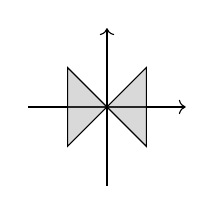
\begin{tikzpicture}
 \draw[->] (0,-1) -- (0,1);
 \draw[->] (-1,0) -- (1,0);
 \draw[fill=gray, fill opacity=0.3] (0,0) -- (0.5,-0.5) -- (0.5,0.5) -- (0,0) -- (-0.5,0.5) -- (-0.5,-0.5) -- cycle;
\end{tikzpicture}\]
\end{example}

\begin{definition}
 Let $R$ be a normed field and let $\mathbb{V}$ be a topological $R$-vector space. We say that $\mathbb{V}$ is \emph{locally convex} iff every $x\in \mathbb{V}$ admits a local basis consisting of disks at $x$.
 Since the topology of $\mathbb{V}$ is necessarily translation invariant,
 it is equivalent to only ask that $0$ has such a local basis.
\end{definition}

The main result is the following:

\begin{proposition}\label{prop:mainLCTVS}
 Let $\mathbb{V}$ be a locally convex topological $\R$-vector space (where $\R$ is endowed with its usual absolute value and the induced topology by it).
 Fix $x\in\mathbb{V}$, a neighbourhood $V\subseteq\mathbb{V}$ of $x$ and $f:V\to \R\cup\set{+\infty,-\infty}$.
 If $V$ is convex, $f$ is concave and lower bounded by a finite constant $K$, then $f$ is continuous at $x$ (w.r.t.\ the subspace topology on $V$).
\end{proposition}
\begin{proof}
 Since $V$ is a neighbourhood of $x$, $x$ admits an open neighbourhood $U\subseteq V$, and by local convexity of $\mathbb{V}$ there is a (non necessary open) disk $D\subseteq U$ at $x$.
 Now fix $\eps\in(0,1)$ and $r,s\in \R$ with $0\leq r\leq\eps$, $s=1-r$.
 Fix also $w\in D$.
 By the convexity of $D$ we have $sx+rw\in D$, and thus the convexity of $f$ entails that:
 \[
  f(sx+rw)\geq s f(x) + r f(w) \geq s f(x) + r K = (1-r)f(x) + r K
 \]
that is,
 \[
  f(x)-f(sx+rw)\leq r (f(x)-K).
 \]
 Now remark that $x=\dfrac{1}{s+2r}(sx+rw)+\dfrac{r}{s+2r}(2x-w)$, where $\dfrac{1}{s+2r}+\dfrac{r}{s+2r}=1$, $\dfrac{1}{s+2r}<1$ and $2x-w\in D$ (because $D$ is a disk at $x$).
 Therefore by the convexity of $f$ we have:
 \[
  f(x)\geq \dfrac{1}{s+2r}f(sx+rw)+\dfrac{r}{s+2r}f(2x-w)\geq \dfrac{1}{s+2r}(f(sx+rw)+rK)
 \]
 that is,
 \[
  f(sx+rw)-f(x)\leq r(f(x)-K).
 \]
 We have thus shown that $\mid f(sx+rw)-f(x)\mid\leq r(f(x)-K)$ for all $w\in D$.
 Since this holds also for all $\eps\in(0,1)$, and due to the choice of $r,s$, the points of shape $sx+rw$ span $D$ when $w$ spans $D$ and $\eps$ spans $(0,1)$.
 That is, we have shown that $\mid f(w)-f(x)\mid\leq r(f(x)-K)$ for all $w\in W$.
 Since $f(x)-K\geq 0$ and $r\leq \eps$, we have that $\exists\lim\limits_{w\to x} f(w)=f(x)$.
\end{proof}

Now we show how to apply this argument to our tropical case $\Lawv^X$, which is \emph{not} a LCTVS (because it is not a vector space).

First, we have:

\begin{corollary}\label{cor:cont}
 Let $f:({\R}_{> 0}^X,\supnorm{.}) \to (\overline\R_{\geq 0},\absv .)$ and $x\in {\R}_{> 0}^X$.
 If there is a convex neighbourhood $V\subseteq \overline{\R}_{> 0}^X$ of $x$ s.t.\ $f_{\lVert V}$ is concave, then $f$ is continuous at $x$.
\end{corollary}
\begin{proof}
 The $\R$-vector space $\R^X$ is topological w.r.t.\ the topology $\tau_\infty$ induced on it by the norm $\lVert .\lVert_\infty$, and it is clearly locally convex.
 Call $\tau^+_\infty$ the topology induced by $\supnorm{.}$ on ${\R}_{> 0}^X$.
 It is clear that it coincides with $\tau^+_\infty$.
 Since moreover ${\R}_{> 0}^X$ is open in $(\R^X,\tau_\infty)$, the neighbourhood $V$ of $x$ in $({\R}_{> 0}^X,\supnorm{.})$ is also a neighbourhood of $x$ in $(\R^X,\tau_\infty)$.
 We can therefore apply Proposition~\ref{prop:mainLCTVS} to $f_{\lVert V}$ (which is lower bounded by $0$ by definition of $f$) and obtain that $f_{\lVert V}$ is continuous at $x$ w.r.t.\ the subspace topology $\tau_V$ induced by $\tau_\infty$ on $V$.
 But since $V$ is contained in ${\R}_{> 0}^X$, the topology $\tau_V$ coincides with the subspace topology induced on $V$ by $\tau^+_\infty$.
 So $f$ is continuous at $x$ w.r.t.\ $\tau^+_\infty$.
\end{proof}

One may wonder if the same proof as above makes it possible to state the previous corollary replacing ${\R}_{> 0}^X$ with $\R_{\geq 0}^X$ (so, in particular, taking $x\in\R_{\geq 0}^X$).
This is not possible because in the proof we crucially use that $\R_{> 0}^X$ is open in $(\R^X,\tau_\infty)$, which is not the case of $\R_{\geq 0}^X$.
In fact, this allowed us to say that $V$ is a neighbourhood of $x$ in $(\R^X,\tau_\infty)$, and therefore to be able to apply Proposition~\ref{prop:mainLCTVS}.
Taking $\R_{\geq 0}^X$ instead, this is in general not true: we could have a neighbourhood of $x$ w.r.t.\ the subspace topology on $\R_{\geq 0}^X$ induced by $\tau_\infty$, which does not contain any open neighbourhood of $x$ w.r.t.\ $\tau_\infty$ (i.e. it is not a neighbourhood w.r.t.\ $\tau_\infty$).

\begin{example}
 An example of a neighbourhood of $x$ w.r.t.\ the subspace topology on $\R_{\geq 0}^X$ induced by $\tau_\infty$, which is not a neighbourhood w.r.t.\ $\tau_\infty$.
 \[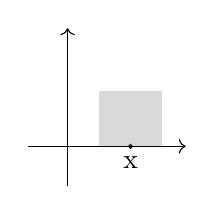
\begin{tikzpicture}
 \draw[->] (0,-0.5) -- (0,1.5);
 \draw[->] (-0.5,0) -- (1.5,0);
 \filldraw[black] (0.8,0) circle (0.7pt) node[anchor=north]{x};
 \fill[fill=gray, fill opacity=0.3] (0.4,0) -- (1.2,0) -- (1.2,0.7) -- (0.4,0.7) -- (0.4,0) -- cycle;
\end{tikzpicture}\]
\end{example}

Finally we have the desired result Theorem~\ref{thm:cont}:

\begin{theorem}[Theorem~\ref{thm:cont}]
 Tropical Laurent series $f:({\R}_{\geq 0}^X,\supnorm .) \to (\overline\R_{\geq 0},\absv .)$ are continuous on ${\R}_{> 0}^X$ w.r.t.\ the norm $\norm{\cdot}_\infty$.
\end{theorem}
\begin{proof}
 We know that tLs's are concave on all their domain.
 Therefore the result immediate follows by Corollary \ref{cor:cont}, since the topology induced by $\supnorm{.}$ on ${\R}_{> 0}^X$ coincides with the subspace topology induced by $({\R}_{\geq 0}^X,\supnorm .)$ on it.
\end{proof}

Due to the previous discussion about the impossibility of stating Corollary \ref{cor:cont} in the case where one of the coordinates of $x$ is $0$, the continuity of tropical functions on the hyperplanes $\mathcal H_a:=\set{x\in {\R}_{\geq 0}^X \mid x_a=0}$, for $a\in X$, must be treated separately.
Similarly, the continuity at points with infinite coordinates must be treated separately as well.
We left it for future investigations.

\begin{remark}
 We formulated the main argument (Proposition~\ref{prop:mainLCTVS}) in the general setting of LCTVS's.
We did so just to show that it is actually a general argument, but we could have placed ourselves already in a more particular setting of our interest and carry on the proof.
For instance, Theorem~\ref{thmTLSlocLip} will be proved by refining this kind of argument (Lemma~\ref{lm:mainLip}), but not in the setting of LCTVS.
\end{remark} 

%\newpage

\begin{definition}
 An \emph{$\overline{\R}_{\geq 0}$-cone} is a commutative $\overline{\R}_{\geq 0}$-semimodule with cancellative addition\footnote{I.e.: $x+y=x+y' \Rightarrow y=y'$.}.
\end{definition}

In [Selinger] cones are required to also have ``strict addition'', meaning that $x+y=0 \Rightarrow x=y=0$.
We do not add this requirement since it will automatic hold when considering normed cones.

\begin{remark}
 The addition of a cone $P$ (which forms a commutative monoid) turns $P$ into a poset by setting:
 \[
  x \leq y \textit{ iff } y=x+z \textit{, for some }z\in P.
 \]
 By the cancellative property, when such $z$ exists it is unique, and we denote it by $y-x$.
 Such order is called the \emph{cone-order} on $P$.
\end{remark}

\begin{definition}
 A \emph{normed $\overline{\R}_{\geq 0}$-cone} is the data of a $\overline{\R}_{\geq 0}$-cone together with a $\leq$-monotone\footnote{I.e.: $x\leq y \Rightarrow \norm{x}\leq \norm y$. Remark that requiring this property (for all $x,y$) is equivalent to requiring that $\norm{x}\leq \norm{x+y}$ for all $x,y$.} norm\footnote{A \emph{norm} on a $\overline{\R}_{\geq 0}$-abstract cone $P$ is a map $\norm{.}:P\to \overline{\R}$ satisfying the usual axioms of norms:
 $\norm x \geq 0$, $\norm x = 0 \Rightarrow x=0$, $\norm{rx}=r\norm x$ and $\norm{x+y}\leq \norm x + \norm y$.} on it.
\end{definition}

In [Ehrhard-Pagani-Tasson, Crubillie] a normed $\overline{\R}_{\geq 0}$-cone is simply called a cone.

Remark that in a normed $\overline{\R}_{\geq 0}$-cone, by monotonicity of the norm, we have: $\norm{x+y}=0 \Rightarrow x=y=0$.
Therefore, as already mentioned, in a normed cone we have: 
$x+y=0 \Rightarrow \norm{x+y}=0 \Rightarrow x=y=0$, that is, addition is strict.

\begin{example}
 $\overline{\R}_{\geq 0}^X$ is a normed cone with the norm $\supnorm{x}:=\sup\limits_{a\in X} x_a\in \overline{\R}_{\geq 0}$.
\end{example}

\begin{remark}
 The cone-order on $\overline{\R}_{\geq 0}^X$ is the pointwise usual order on $\overline{\R}_{\geq 0}$.
 
 Remark also that tropical functions have no reason to be linear nor sublinear.
\end{remark}

\begin{remark}\label{rmk:tropMonot}
 Tropical functions are monotone w.r.t.\ to the cone order on its domain and codomain.
 This is clear, using the definition of tropical functions, because $\mu x\leq \mu y$ if $x\leq y$.
\end{remark}

\begin{remark}
 The cone-order on $\overline{\R}_{\geq 0}^X$ makes it into a dcpo with least element $0$.
\end{remark}

The following is a usual domain theoretical lemma.

\begin{lemma}\label{lm:sup=sup}
 Let $P$ be a poset and $X, I$ sets. Fix the pointwise order on $P^X$.
 \begin{enumerate}
  \item Let $x^i\in P^X$ for $i\in I$.
  If $\bigvee\limits_{i\in I} x^i$ exists $P^X$, then $\bigvee\limits_{i\in I} x^i_a$ exists in $P$ for all $a\in X$, and we have: $\bigvee\limits_{i\in I} x^i_a=\left(\bigvee\limits_{i\in I} x^i\right)_a$.
 \item Let $x^i_a\in P$ for $i\in I,a\in X$.
  If $\bigvee\limits_{i\in I} x^i_a$ exists $P$ for all $a\in X$, then $\bigvee\limits_{i\in I} x^i$ exists in $P^X$, and we have: $\left(\bigvee\limits_{i\in I} x^i\right)_a=\bigvee\limits_{i\in I} x^i_a$.
 \end{enumerate}
\end{lemma}

A \emph{directed net} in a poset $P$ with indices in a set $I$ is a function $s:I\to P$, denoted by $(s_i)_{i\in I}$, s.t.\ its image is directed.
We say that a directed net in $P$ \emph{admits a sup} iff its image admits a sup in $P$.
We say that a directed net $s$ in a normed cone is \emph{bounded} iff the set $\set{\norm{s_i}\,\mid i\in I}$ is bounded in $\R_{\geq 0}$.

Remember the definition of Scott-continuity:

\begin{definition}
 A function $f:P\to P'$ between posets is \emph{Scott-continuous} iff for all directed net $(s_i)_i$ in $P$ admitting a sup, we have $\exists \bigvee\limits_i f(s_i) = f(\bigvee\limits_i s_i)$ in $P'$. 
\end{definition}

The fundamental result in order to prove Theorem~\ref{thm:ScottCont} is the following, taken from [Selinger].

\begin{proposition}\label{prop:infsup}
 Let $P$ be a normed $\overline{\R}_{\geq 0}$-cone s.t.\ every bounded directed net in $P$ admits a sup.
 Let $(v_i)_{i\in I}$ be a directed net in $P$ with an upper bound $v\in P$.
 Then $\exists\bigvee\limits_{i\in I} v_i \in P$ and, if $\inf\limits_{i\in I} \norm{v-v_i} =0$, one has: $\bigvee\limits_{i\in I} v_i = v$.
\end{proposition}
\begin{proof}
 Remark that $v-v_i$ exists in $P$ by hypothesis and so does $\bigvee\limits_{i\in I} v_i$, thanks to the monotonicity of the norm.
 Now, since $v\geq v_i$ for all $i$, we have that $v\geq \bigvee\limits_{i\in I} v_i$, and so $v-\bigvee\limits_{i\in I} v_i$ exists in $P$.
 Fix $i\in I$.
 Since $v_i\leq \bigvee\limits_{i\in I} v_i$, then $v-\bigvee\limits_{i\in I} v_i\leq v-v_i$ and, by monotonicity of the norm, $\norm{v-\bigvee\limits_{i\in I} v_i}\leq \norm{v-v_i}$.
 Since this holds for all $i\in I$, we have:
 $0\leq \norm{v-\bigvee\limits_{i\in I} v_i}\leq \inf\limits_{i\in I} \norm{v-v_i}=0$, where the last equality holds by hypothesis.
 Thus $\norm{v-\bigvee\limits_{i\in I} v_i}=0$, i.e.\ $v=\bigvee\limits_{i\in I} v_i$.
\end{proof}

\begin{definition}
 A normed $\overline{\R}_{\geq 0}$-cone $P$ is \emph{Scott-complete} iff its norm is Scott-continuous (where the codomain $\overline\R_{\geq 0}$ is endowed with its usual order) and every bounded directed net in $P$ admits a sup.
 This is equivalent to asking that its closed unit ball is a dcpo.
\end{definition}

\begin{proposition}
 The normed cone $\overline{\R}_{\geq 0}^X$ is Scott-complete.
\end{proposition}
\begin{proof}
 $\overline{\R}_{\geq 0}^X$ being a dcpo, all the existences of sup's that we should check do automatically hold, so we only have to show that $\bigvee$ and $\supnorm{.}$ commute:
 $\supnorm{\bigvee\limits_i x_i}=
 \sup\limits_a\, \sup\limits_i\, (x_i)_a =
 \sup\limits_i\, \sup\limits_a\, (x_i)_a =
 \bigvee\limits_i \supnorm{x_i}$.
\end{proof}

%Let us set $\infty_b$ to be the hyper-semi-plane $\set{y\in\overline{\R}^Y_{\geq 0}\mid y_b=+\infty}$ and $\set{f<<+\infty}:=\bigcup\limits_{b\in Y} f^{-1}\infty_b$.

%\begin{remark}\label{rmk:R-f<<oo}
%Let $f:\overline{\R}^X_{\geq 0}\to\overline{\R}^Y_{\geq 0}$ be tropical.
%Then, $\R^X_{> 0}-\set{f<<+\infty}$ is a dcpo (w.r.t.\ the usual order, that is, its cone order).
%In order to see this, it is enough to show that, for any $b\in Y$ and for any directed net $(x^i)_i$ in $\R^X_{> 0}$ s.t.\ $f(x^i)_b<+\infty$ for all $i$, we have $f(\bigvee\limits_i x^i)_b<+\infty$ (where the sup is taken in $\R^X_{> 0}$).
%Such property holds because otherwise it is easy to see that $f$ would be discontinuous at the point $\bigvee\limits_i x^i\in\R^X_{> 0}$ w.r.t.\ the topology\footnote{Remark that this argument would not be possible using Scott-continuity instead. Indeed, it could well be that $f(\bigvee\limits_i x^i)_b=\bigvee\limits_i f(x^i)_b=+\infty$ while $f(x^i)_b<+\infty$ for all $i$.} induced by $\supnorm{.}$.
%This contradicts Corollary \ref{cor:tropCont}.
%\end{remark}

\begin{proposition}
 All tropical functions $f:\overline{\R}^X_{\geq 0}\to\overline{\R}^Y_{\geq 0}$ are Scott-continuous on $\R^X_{> 0}$ w.r.t.\ the cone-orders on its domain and codomain.
\end{proposition}
\begin{proof}
 Let $(x_i)_i$ a directed net in $\R^X_{> 0}$ s.t.\ $\bigvee\limits_i x^i$ exists in $\R^X_{> 0}$.
 Then $\inf\limits_i \supnorm{\bigvee\limits_i x^i - x^i} =0$, where $\bigvee\limits_i x^i - x^i$ exists because $\bigvee\limits_i x^i \geq x^i$ for all $i$.
 Since $f$ is $\supnorm{.}$-continuous on $\R^X_{> 0}$ (Corollary \ref{cor:tropCont}), then $\inf\limits_i \supnorm{f(\bigvee\limits_i x^i) - f(x^i)} =0$, where $f(\bigvee\limits_i x^i) - f(x^i)$ exists because $f(\bigvee\limits_i x^i) \geq f(x^i)$ for all $i$ being $f$ monotone (Remark \ref{rmk:tropMonot}).
 We can therefore apply Proposition \ref{prop:infsup} to the directed net $(f(x^i))_i$ in $\overline{\R}^Y_{\geq 0}$, obtaining that $\bigvee\limits_i f(x^i)$ exists in $\overline{\R}^Y_{\geq 0}$ and it coincides with $f(\bigvee\limits_i x^i)$.
\end{proof}

%\begin{remark}
%By looking at the definition of tropical functions, for $f$ tropical we have that: if $x,x'\in\R^X_{> 0}-\set{f<<+\infty}$ and $r\in\R_{> 0}$, then $x+x',rx\in\R^X_{> 0}-\set{f<<+\infty}$.
%That is, $\R^X_{> 0}-\set{f<<+\infty}$ is a $\R_{>0}$-cone.
%It is clearly still Scott-complete.
%\end{remark}

In the main paper we mention that $\R_{\geq0}^X$ is a Scott-complete dcpo.
We did not state it as a theorem because it follows from standard and well-known domain theoretical considerations.
Let us prove it here anyway.

Recall the definition of Scott-complete dcpo:

\begin{definition}
 Let $P$ be a dcpo and define a relation by: $x<<y$ iff for all directed $D\subseteq P$, if $y\leq \bigvee D$, then $x\leq d$, for some $d\in D$.
 Call $\twoheaddownarrow y:=\set{x\in P\mid x<<y}$.
 A dcpo $P$ is \emph{Scott-continuous} iff $\twoheaddownarrow x$ is directed and $x=\bigvee\twoheaddownarrow x$ for all $x\in P$.
\end{definition}

\begin{remark}
 In any dcpo we have: $\twoheaddownarrow x \subseteq \downarrow x$.
 This immediately follows by considering the directed set $\set{x}$.
\end{remark}

\begin{lemma}\label{lm:<<dir}
 In $\overline{\R}_{\geq 0}^X$, every set $\twoheaddownarrow x$ is directed.
\end{lemma}
\begin{proof}
 It is immediate that $0\in\twoheaddownarrow x$, so it is non-empty.
 Now let $y,y' << x$.
 Since we are in $\overline{\R}_{\geq 0}^X$, there is $y\vee y'\in\overline{\R}_{\geq 0}^X$.
 So we only have to show that $y\vee y'<<x$.
 For that, let $D$ be a directed set in $\overline{\R}_{\geq 0}^X$ s.t.\ $x\leq\bigvee D$.
 Since $y,y' << x$ we find $d,d'\in D$ s.t.\ $y\leq d$, $y'\leq d'$.
 Since $D$ is directed, there is $\hat d\in D$ s.t.\ $y\leq d\leq \hat d\geq d'\geq y'$.
 But then, by definition of sup, it must be $\hat d\geq y\vee y'$ and we are done.
\end{proof}

\begin{remark}
 The following is a known property (that we will not use):
 let $P$ be a complete normed cone which is a dcpo w.r.t.\ its cone-order. Then $P$ is Scott-continuous as a dcpo iff its closed unit ball is Scott-continuous as a dcpo.
\end{remark}

\begin{remark}\label{rmk:<<R}
 Consider $\overline{\R}_{\geq 0}$ with its usual order (which coincides with its cone-order).
 It is easily seen (and well known) that $y<<x$ iff either $y=0$ or $y<x$.
 This immediately implies that $\overline{\R}_{\geq 0}$ is Scott-continuous, since $x=\sup\limits_{y<x} y$.
\end{remark}

\begin{lemma}\label{lm:<<RX}
 Let $x,y\in \overline{\R}_{\geq 0}^X$ (considered as a dcpo with its cone order, which is the pointwise one). Fix $a\in X$.
 If $y_a<<x_a$ and $y_c=0$ for all $c\neq a$, then $y<<x$.
\end{lemma}
\begin{proof}
 Towards a contradiction, assume that there is a directed set $D$ in $\overline{\R}_{\geq 0}^X$ with $x\leq\bigvee D$ and s.t.\ $y\not\leq d$ for all $d\in D$.
 Call $D_a:=\set{d_a\mid d\in D}$ and remark that it is directed, because $D$ is.
 Also, by Lemma \ref{lm:sup=sup}, $\bigvee D_a = \left(\bigvee D\right)_a$.
 Therefore from $y_a<<x_a\leq \bigvee D_a$ we obtain a $d\in D$ s.t.\ $y_a\leq d_a$.
 By the absurd hypothesis we have $y\not\leq d$, so there must be $c\in X$ s.t.\ $y_c\not\leq d_c$, i.e. (because real numbers are totally ordered) $y_c>d_c$.
 Therefore it must be $c\neq a$.
 But then we have $0=y_c>d_c\geq 0$, contradiction.
\end{proof}

\begin{lemma}\label{lm:<<_a}
 In $\overline{\R}_{\geq 0}^X$ we have:
 if $y<<x$ then $y_a<< x_a$ for all $a\in X$.
\end{lemma}
\begin{proof}
 Fix $a\in X$.
 Let $D$ directed set in $\overline{\R}_{\geq 0}$ s.t.\ $x_a\leq\bigvee D$.
 We look for a $d\in D$ s.t.\ $y_a\leq d$.
 For $d\in D$, let $x^{a,d}\in\overline{\R}_{\geq 0}^X$ defined by $x^{a,d}_c:=x_c$ if $c\neq a$ and $x^{a,d}_a:=d$.
 Let $D^x_a:=\set{x^{a,d}\mid d\in D}$.
 By Lemma \ref{lm:sup=sup} $D^x_a$ admits sup in $\overline{\R}_{\geq 0}^X$ and it is $(\bigvee D^x_a)_c=x_c$ if $c\neq a$ and $(\bigvee D^x_a)_a=\bigvee D$.
 Hence, $x\leq \bigvee D^x_a$.
 If we prove that $D^x_a$ is directed, we are done: indeed, since $y<<x$, there is $d\in D$ s.t.\ $y\leq x^{a,d}$ and thus, in particular, $y_a\leq x^{a,d}_a=d$.
 Let us finally prove that $D^x_a$ is directed: it is clearly non-empty, since $D$ is.
 Let now $d,d'\in D$.
 We want to show that there is $\hat d\in D$ s.t.\ $x^{a,d}\leq x^{a,\hat d}\geq x^{a,d'}$.
 But since $D$ is directed, there is $\hat d\in D$ s.t.\ $d\leq \hat d\geq d'$, and therefore $x^{a,d}_c=x_c= x^{a,\hat d}_c =x_c=x^{a,d'}_c$ for all $c\neq a$, and $x^{a,d}_a=d\leq \hat d=x^{a,\hat d}_a=\hat d \geq d'=x^{a,d'}_a$.
\end{proof}

\begin{lemma}\label{rmk:sup_a=sup_a}
In $\overline{\R}_{\geq 0}^X$ we have:
$\bigvee\limits_{y<<x_a} y = \bigvee\limits_{y<<x} y_a$.
\end{lemma}
\begin{proof}
 If we show that $\twoheaddownarrow x_a = \set{y_a\mid y\in\twoheaddownarrow x}$, then we are done because in the statement we are taking their sup's.
 The inclusion ($\supseteq$) immediately follows from Lemma \ref{lm:<<_a}. For ($\subseteq$), let $d<< x_a$.
 Then the $y\in \overline{\R}_{\geq 0}^X$ defined by $y_c:=0$ if $c\neq a$ and $y_a:=d$, is s.t.\ $y\in\twoheaddownarrow x$ by Lemma \ref{lm:<<RX}.
 Thus, $d\in \set{y_a\mid y\in\twoheaddownarrow x}$.
\end{proof}


\begin{corollary}
 The dcpo $\overline{\R}_{\geq 0}^X$ is Scott-continuous.
\end{corollary}
\begin{proof}
 The fact that $\twoheaddownarrow x$ is directed is given by Lemma \ref{lm:<<dir}. The fact that $x=\bigvee \twoheaddownarrow x$ is given by the following equalities:
 $x_a=\bigvee\limits_{y<<x_a} y = \bigvee\limits_{y<<x} y_a = \left(\bigvee\limits_{y<<x} y\right)_a=\left(\bigvee \twoheaddownarrow x\right)_a$.
 The first equality follows from Remark \ref{rmk:<<R}, the second one from Lemma \ref{rmk:sup_a=sup_a}, the third one from Lemma \ref{lm:sup=sup}.
\end{proof}

\newpage



\subsubsection{Lipschitz continuity}





  We need a first, preliminary, lemma:
\begin{lemma}\label{lemma:inf}
Let $u,v: I\to Q$ and suppose $|u(i)-v(i)|\leq \delta$, for all $i\in I$.
Then $|\inf_{i\in I}u(i)- \inf_{i\in I}v(i)|\leq \delta$. 
\end{lemma}
\begin{proof}
Let $A=\inf_{i\in I}u(i)$ and $B=\inf_{i\in I}v(i)$ and suppose $A\geq B$. 
Suppose by way of contradiction $|A-B|> \delta$; then there exists $i\in I$ such that 
$v(i)<A$ and $|A-v(i)|> \delta$. Indeed, otherwise we would have $|A-B|= \sup\{ |A-v(i)|\mid v(i)\leq A\}\leq \delta$. 
Now, from $|A-v(i)|> \delta$ and $v(i)< A$ we deduce that $|u(j)-v(i)|> \delta$ for all $j\in I$, and thus in particular that $|u(i)-v(i)|>\delta$, against the assumption. We conclude then $|A-B| \leq \delta$.
In case $B\geq A$, we can argue in a similar way. 
\end{proof}



\begin{proposition}\label{prop:troplinear}
All tropical linear functions $f: \Lawv^{X}\to \Lawv^{Y}$ are non-expansive.  
\end{proposition}
\begin{proof}
%All functions of the form $f_{\theta,\eta}(x)_{b}= \theta(b)+x_{\eta(b)}$, where $\theta:Y \to \Lawv$ and $\eta:Y\to X$, are non-expansive: indeed $|f_{\theta,\eta}(x)_{b}-f_{\theta,\eta}(y)_{b}|= |\theta(b)+x_{\eta(b)}-\theta(b)-y_{\eta(b)}|=
%|x_{\eta(b)}-y_{\eta(b)}|\leq \norm{x-y}_{\infty}$.
Let $f(x)_{b}=\inf_{a}\{\widehat f_{a,b}+x_{a}\}$.
For all $a\in X$ we have that 
$|(\widehat f_{a,b}+x_{a})- (\widehat f_{a,b}+y_{a})|=
|x_{a}-y_{a}|\leq \norm{x-y}_{\infty}$. Using Lemma \ref{lemma:inf}, we deduce then 
$|f(x)_{b}-f(y)_{b}|=|\inf_{a}\{\widehat f_{a,b}+x_{a}\}-
\inf_{a}\{\widehat f_{a,b}+y_{a}\}|\leq \norm{x-y}_{\infty}$.
\end{proof}






\begin{lemma}\label{lm:mainLip}
Let $f: [0,\infty)^{X}\to Q$ be concave, monotone increasing, and continuous.  
Let $ x \neq  y  \in [0,\infty)^{X}$, with $\| x - y  \|_{\infty}<\infty$, and let $S( x ,  y  )=\{ \alpha x  + (1-\alpha) y  \mid \alpha \in [0,1]\}$ be the segment generated by $ x $ and $ y  $. 
Then $f$ is Lipschitz-continuous over $S( x ,  y  )$.

\end{lemma}
\begin{proof}
Let us prove the lemma under the assumption that for all $a\in X$, $ y  _{a}- x _{a}\geq 1$. From the fact that the claim holds under the assumption, we can deduce the claim of the lemma:
indeed for $\alpha\in (0,1)$ large enough we have that $ y  ':= \frac{ y  -\alpha x }{1-\alpha}$ is such that $ y  \in S( x ,  y  ')$ (and thus $S( x ,  y  )\subseteq S( x ,  y  ')$) and 
$ y  '_{a}- x _{a}\geq 1$. Hence from our proof we deduce that $f$ is Lipschitz-continuous over $S( x ,  y  ')$, and thus a fortiori over $S( x ,  y  )$ too.


Since $f$ is continuous over $[0,\infty)^{X}$ and $S( x ,  y  )$ is compact, $f$ admits a maximum $\mathrm{MAX}$ over $S( x ,  y  )$.
For all $ z  <  z  '\in S( x ,  y  )$, let $M( z  ,  z  ')\in Q^{X}$ be defined by
$$
M( z  ,  z  ')_{a}= \frac{f( z  ')-f( z  )}{ z  '_{a}- z  _{a}}
$$
Observe that
\begin{align*}
M( x ,  y  )_{a} & = \frac{f( y  )-f( x )}{ y  _{a}- x _{a}} \leq 
f( y  )-f( x ) \leq \mathrm{MAX}
\end{align*}
using the fact that $ y  _{a}- x _{a}\geq 1$. 

We now claim that $M( z  ,  z  ')$ is contravariant in both $ z  $ and $ z  '$. 
Indeed suppose $ z  \leq  z  '' <  z  '$, so that $ z  = \lambda  z  ' +(1-\lambda) z  ''$ for some $\lambda \in (0,1)$. Then, using the fact that $f$ is concave, we have 
\begin{align*}
M( z  ,  z  ')_{a}&=\frac{f( z  ')-f(\lambda  x  +(1-\lambda) z  '')}{ z  '_{a}-\lambda  x _{a} -(1-\lambda) z  ''_{a}} \\
&
\geq 
\frac{f( z  ')-\lambda f( z  ') -(1-\lambda)f( z  '')}{ z  '_{a}-\lambda  z  '_{a} -(1-\lambda) z  ''_{a}} \\
&
= 
\frac{(1-\lambda)(f( z  ')-f( z  ''))}{(1-\lambda ) z  '_{a}- z  ''_{a}} =M( z  '',  z  ')
\end{align*}
In a similar way it is shown that for $ z   <  z  ''\leq  z  '$, $M( z  , z  ')\leq M( z  ,  z  '')$. 

Therefore, for all $ z   <  z  '\in S( x ,  y  )$, we have that $M( z  ,  z  ')_{a} \leq M( x ,  z  ')_{a} \leq M( x ,  y  )_{a} \leq \mathrm{MAX}$. 
From this, using the fact that $f$ is monotone increasing, we deduce that 
$|f( z  ')-f( z  )|=f( z  ')-f( z  ) \leq \mathrm{MAX}\cdot | z  '_{a}- z  _{a}|
$ and thus that 
$$|f( z  ')-f( z  )|\leq \mathrm{MAX}\cdot \| z  '- z  \|_{\infty}$$
that is, that $f$ is $\mathrm{MAX}$-Lipschitz over $S( x ,  y  )$. 
\end{proof}

\begin{proposition}
Let $f: [0,\infty)^{X}\to Q$ be concave, monotone increasing, and continuous.  
For all $\epsilon \in (0,\infty)$ and $ x \in [0,\infty)^{X}$, $f$ is Lipschitz-continuous over the open ball $B( x , \epsilon)$.
\end{proposition}
\begin{proof}
Let $\mathrm{MAX}$ indicate the maximum of $f$ over $B( x , \epsilon)$. 
Let $ y  ,  z  \in B( x , \epsilon)$; then $\| y  - z  \|_{\infty}\leq 2\epsilon < \infty$, so by the lemma above $f$ is $K$-Lipschitz over the segment $S( y  ,  z  )$ for some $K\leq \mathrm{MAX}$, so we deduce $|f( y  )-f( z  )|\leq \mathrm{MAX}\cdot \| y  - z  \|_{\infty}$.
\end{proof}

\begin{theorem}[local Lipschitz-continuity]
Let $f: [0,\infty)^{X}\to Q$ be concave, monotone increasing, and continuous.  
Then $f$ is locally Lipschitz-continuous.
\end{theorem}
\begin{proof}
For all $ x \in [0,\infty)^{X}$, $f$ is Lipschitz-continuous over the open set $B( x , 1)$.
\end{proof}



\subsubsection{Characterizations of the functional metric }



  \begin{proposition}\label{prop:functionalmetric}
For all maps $f,g: Q\langle X\rangle\to Q\langle Y\rangle$,  
$$
  \|\widehat f- \widehat g\|_{\infty}=
  \sup\{\|f( x )- g( x )\|_{\infty} \mid  x \in Q\langle X\rangle\}
$$

\end{proposition}
  
%
%\begin{lemma}
%Let $f,g\in\mathsf{Trop}(1,1)$ (i.e.~$f,g:Q\to Q$), and suppose for all $n\in \BB N$, 
%$|\widehat f_{n}-\widehat g_{n}|\leq \delta$. Then for all $x\in Q$, $|f(x)-g(x)|\leq \delta$.
%
%\end{lemma}
%\begin{proof}
%$|f(x)-g(x)|= |( \inf_{n}nx+\widehat f_{n})- (\inf_{n}nx+\widehat g_{n})|$. 
%Since $|nx+\widehat f_{n} - nx -\widehat g_{n}|= |\widehat f_{n}-\widehat g_{n}|\leq \delta$, by the Lemma above we conclude $|f(x)-g(x)|\leq \delta$. 
%\end{proof}



  
  \begin{proof}[Proof of Proposition \ref{prop:functionalmetric}]
For one side, suppose for all $\mu\in \C  M_{\mathrm{fin}}(X),b\in Y$, 
$|\widehat f_{\mu,b}-\widehat g_{\mu,b}|\leq \delta$. Then for all $ x \in Q\langle X\rangle$ and $b\in Y$, $|f( x )(b)-g( x )(b)|\leq \delta$.
Indeed, $|f( x )(b)-g( x )(b)|= |( \inf_{\mu}\mu  x +\widehat f_{\mu,b})- (\inf_{\mu}\mu  x +\widehat g_{\mu,b})|$. 
Since $|\mu  x +\widehat f_{\mu,b} - \mu  x  -\widehat g_{\mu,b}|= |\widehat f_{\mu,b}-\widehat g_{\mu,b}|\leq \delta$, by Lemma \ref{lemma:inf} we conclude $|f( x )(b)-g( x )(b)|\leq \delta$. 


For the other side, suppose for some $\mu\in \C M_{\mathrm f}(X)$ and $b\in Y$, $|\widehat f_{\mu,b}-\widehat g_{\mu,b}|> \epsilon$; 
then, by letting $e_{\mu}\in Q\langle !X\rangle$ be the (tropical) characteristic function of $\mu$, we have
 $|f(e_{\mu})({b})-g(e_{\mu})({b})| =
|( \inf_{\mu'}\widehat f_{\mu',b}+ \mu'(e_{\mu}))-
( \inf_{\mu'}\widehat g_{\mu',b}+\mu'(e_{\mu}))|=
|\widehat f_{\mu,b}- \widehat g_{\mu,b}|> \epsilon$, so we deduce that 
$\sup\{\| f( x )- g( x ) \|_{\infty}\mid  x \in Q\langle X\rangle\}> \epsilon$.
\end{proof}


The second characterization relates distances with the Taylor expansion. Let us briefly discuss the latter, first.
For all $f: Q\langle X\rangle \to Q\langle Y\rangle$, let $\delta^{(n)}f:Q\langle X^{n}\rangle \to Q\langle Y\rangle$ indicate the $n$-linear function given by 
$$
\delta^{(n)}f( x ^{n})= D^{(n)}f( x ^{n}, \infty)
$$

Notice that $\widehat{\delta^{(n)}f}\in Q^{X^{n}\times Y}$ satisfies 
$\widehat{\delta^{(n)}f}_{a_{1},\dots, a_{n},b}= \widehat f_{[a_{1},\dots, a_{n}],b}$.
In other words, $\delta^{(n)}f$ precisely captures the behavior of $f$ when applied to multisets of length $n$. Moreover, the full behavior of $f$ can be recovered from the functions $\delta^{(n)}f$ using the Taylor expansion which, in its tropical form, reads as:
\begin{equation*}
f( x )= \inf_{n}\left \{ D^{(n)}f( x ^{n},\infty)\right\}= \inf_{n}\left \{\delta^{(n)}f( x ^{n})\right\}
%\tag{Tropical Taylor}
\end{equation*}





\begin{proposition}\label{prop:taylormetric}
For all $f,g:Q\langle X\rangle \to Q\langle Y\rangle$, 
$$
\| \widehat f-\widehat g\|_{\infty}= \sup_{n}\| \widehat{\delta^{(n)}f} -\widehat{\delta^{(n)}g}\|_{\infty}
$$
\end{proposition}
\begin{proof}
Let us first show that $\| \widehat f-\widehat g\|_{\infty}\leq \epsilon$ implies 
$\| \delta^{(n)}f-\delta^{(n)}g\|_{\infty}\leq\epsilon$, for all $n\in \BB N$. 
Notice that $\widehat{\delta^{(n)}f}\in Q^{X^{n}\times Y}$ satisfies 
$\widehat{\delta^{(n)}f}_{a_{1},\dots, a_{n},b}= \widehat f_{[a_{1},\dots, a_{n}],b}$. Hence 
from $\| \widehat f-\widehat g\|\leq\epsilon$ it follows that for all $\mu=[a_{1},\dots, a_{n}]$ and $b\in Y$, 
$|\widehat f_{\mu,b}- \widehat g_{\mu,b}|\leq \epsilon$, so 
we deduce that $\| \widehat{\delta^{(n)}f}- \widehat{\delta^{(n)}g}\|\leq \epsilon$.

For the converse direction suppose that, for all $n\in \BB N$, $\| \widehat{\delta^{(n)}f}- \widehat{\delta^{(n)}g}\|\leq \epsilon_{n}$. Then, since the family of coefficients $
F_{n,\mu,b}=
( \widehat{\delta^{(n)}f})_{a_{1},\dots, a_{n},b}$ (where $\mu=[a_{1},\dots, a_{n}]$) is in bijection with the coefficients $\widehat f_{\mu,b}$, we deduce that $|\widehat f_{\mu,b}-\widehat g_{\mu,b}|\leq 
\epsilon_{\sharp \mu  }$, and thus that 
$\| \widehat f-\widehat g\|_{\infty}\leq \sup_{n}\epsilon_{n}$. 
\end{proof}



\newpage
\subsection{Proofs from Section VII}
%
\begin{remark}\label{rem:functor}
Given $f:X\to Q$, $f$ is a functor precisely when for all $x,y\in X$ $f(x)\leq\inf_{x'\in X}f(x')+X(x',x)$. 
Indeed, if $f$ is a functor then $f(x)\leq f(x')+X(x',x)$, since $f(x)-f(x')=Q(f(x'),f(x))\leq X(x',x)$. 
Conversely, if $f(x)\leq f(x')+X(x',x)$ holds for all $x'$, then 
$Q(f(x),f(x'))=f(x')-f(x)\leq X(x',x)$. 
\end{remark}



\begin{remark}[Yoneda embedding]
%$\Lawv$ is a $\Lawv$-category with $Q(x,y)=|x-y|$. 
%For any $\Lawv$-category $X$ we can define a new $\Lawv$-category $\mathsf{Dist}(X,Q)$ (that we note simply as $[X,Q]$) whose objects are the distributors $x:\{\star\}\pfun X$, or equivalently, the functors from $X$ to $\Lawv$, i.e.~those $x\in \Lawv^{X}$ such that $|x_{a}-x_{b}|\leq X(a,b)$, or equivalently $x_{a}+X(a,b) \geq x_{b}$.


The \emph{Yoneda embedding} is the faithful functor $\B Y: X\to [X,Q]$ given by $\B Y(x)(y)=X(y,x)$. The functoriality and faithfulness of $\B Y$ follow from
\begin{align}
[X,Q](\B Y(x),\B Y(x'))= X(x,x') \tag{Yoneda}
\end{align}
which is proved as follows: for all $y\in X$ we have 
\begin{align*}
Q( \B Y(x)(y),\B Y(x')(y))&= \B Y(x')(y)-\B Y(x)(y) \\
&= X(y,x')-X(y,x) \leq X(x,x')
\end{align*}
where the last step follows from $X(y,x)+X(x,x')\geq X(y,x')$. 
From this we deduce that $[X,Q](\B Y(x),\B Y(x'))=\sup_{y\in X}Q( \B Y(x)(y),\B Y(x')(y))\leq X(x,x')$. 
For the converse direction, we have  
\begin{align*}
X(x,x') &  = X(x,x') - 0 \\ &=
X(x,x')- X(x,x)
\\& =\B Y(x')(x)-\B Y(x)(x)= Q(\B Y(x)(x),\B Y(x')(x))\\
&\leq [X,Q](\B Y(x), \B Y(x'))
\end{align*}
\end{remark}


\begin{remark}
The \emph{opposite Yoneda embedding} is the faithful functor
$\B Y^{\mathrm{op}}: X\to [X,Q]^{\mathrm{op}}$ given by $\B Y^{\mathrm{op}}(x)(y)=X(x,y)$. The functoriality and faithfulness of $\B Y^{\mathrm{op}}$ follow from
\begin{align}\label{eq:yonedaop}
[X,Q](\B Y^{\mathrm{op}}(x),\B Y^{\mathrm{op}}(x'))= X(x',x) \tag{Yoneda$^{\mathrm{op}}$}
\end{align}
which is proved similarly to the case of $\B Y$.
\end{remark}

\subsubsection{completeness}






Composition with $r:X\pfun Y$ yields a functor
$$
r\cdot \_ : \LREL(A,X)   \longrightarrow \LREL(A,Y)
$$
which
has a right-adjoint
$$
\_ \multimapinv r : \LREL(A,Y)   \longrightarrow \LREL(A,X)
$$
given, for $s:A\pfun Y$ by 
\begin{align*}
(s\multimapinv r)(a,x)= \sup_{y\in Y}s(a,y) \dotdiv r(x,y)
%(R\multimap S)(a,x)= \sup_{y\in Y}
\end{align*}




%
%
%Let $\Phi:Y\pfun Z$ be a distributor and $f:Y\to X$ be a functor.
%A functor $ g:Z\to X$ is called the \emph{$\Phi$-weighted colimit of $f$} if it satisfies, for all
%$z\in Z$ and 
% $x\in X$, 
%$$
%X(g(z), x) \ = \  \sup_{y\in Y}X(f(y),x) - \Phi(y,z)
%$$
%If this colimit exists, we write it as $\mathrm{colim}(\Phi,f)$.
%
%
%A $\Lawv$-category $X$ is said \emph{complete} if it admits all weighted colimits, and a functor $f:X\to Y$ of $\Lawv$-categories is said \emph{continuous} if it commutes with all weighted colimits, meaning that $f \circ \mathrm{colim}(\Phi,g)= \mathrm{colim}(\Phi, f\circ g)$.
%
%
%
%We let $\GMet$ indicate the category of skeletal and complete $\Lawv$-categories and continuous functors. 
%
%

For a $\Lawv$-category $X$, we write $x\simeq y$ when $X(x,y)=X(y,x)=0$. $\simeq$ coincides with $=$ precisely when $x$ is skeletal.

\begin{proposition}\label{prop:yonedasup}
Let $X$ be a skeletal $\Lawv$-category. Then $X$ is complete iff the Yoneda embedding has a left-adjoint.
\end{proposition}
\begin{proof}
 For all $ x\in [X,Q]$, let $\sup x$ be defined as a weighted colimit via
$$
X(\sup x, b)= \sup_{a\in X} X(a,b)-x_{a}
$$
that is, $\sup  x= \mathrm{colim}(  x, \mathrm{id}_{X})$, where $ x$ is seen as a distributor $x:\{\star\}\pfun X$.


Let us check that $\sup: [X,Q]\to X$ is a functor. First, let us check the  inequality
\begin{align}\label{eq:in1}
(X\multimapinv y)\cdot ( y\multimapinv x)\geq (X\multimapinv x)\end{align}
as follows:
\begin{align*}
\left((X\multimapinv  y)\cdot ( y\multimapinv x)\right)(a)&=
 \left (\sup_{b}X(b,a)- y_{b}\right)+\left(\sup_{b} y_{b}-x_{b}\right)\\
&\geq
\sup_{b}(X(b,a)- y_{b})+( y_{b}-x_{b})
\\
&=\sup_{b}(X(b,a)- y_{b}+ y_{b})-x_{b}
\\
&=\sup_{b} X(b,a)-x_{a}\\
&= (X\multimapinv x)(a)
\end{align*}
From \eqref{eq:in1} we deduce immediately the inequality below:
\begin{align}\label{eq:in2}
 y\multimapinv x \geq (X\multimapinv x)\multimapinv(X\multimapinv y)
\end{align}
and we can now compute:
\begin{align*}
[X,Q](x,  y)&= \sup_{a\in X} y_{a}-x_{a}\\
 &\stackrel{\tiny\eqref{eq:in2}}{\geq}
 \sup_{a\in X} \left( \sup_{b\in X}X(b,a)-x_{a}\right) -\left(  \sup_{b\in X}X(b,a)- y_{a}   \right )\\
 &= \sup_{a\in X}X(\sup x, a)-X(\sup  y, a)\\
 &= [X,Q](\B Y^{\mathrm{op}}(\sup y),\B Y^{\mathrm{op}}(\sup x))
 \tag{\ref{eq:yonedaop}}
 \\
&=X(\sup x, \sup  y)
\end{align*}


Then for all $x\in X$, $\sup \B Y(x)\simeq x$. Indeed we have 
\begin{align*}
X(\sup \B Y(x), y) & = \sup_{z\in X}X(z,y) -\B Y(x)(z) \\
& = \sup_{z\in X}X(z,y)-X(z,x)\\
&= X(x,y)
\end{align*}
%where we use the fact that from $X(x,y)+X(z,x) \geq X(z,y)$ it follows $X(x,y) \geq X(z,y)-X(z,x)$ and thus $X(x,y) \geq \sup_{z}X(z,y)-X(x,z)$, and conversely, from $X(x,y)-X(x,x)=X(x,y)$ it follows
%%$X(x,y) \leq \sup_{z}X(z,y)-X(x,z)$.
%

Moreover, for all $x\in [X,Q]$, we have $\B Y(\sup x)\geq x$:  
\begin{align*}
\B Y(\sup x)(a) &= X(a,\sup x)\\
&= X(  \sup(\B Y(a)),\sup x) \\
& \geq [X,Q]( \B Y(a), x)\\
&\geq x_{a}-\B Y(a)(a) \\
&=
 x_{a}-X(a,a)  = x_{a}
\end{align*}
%where in the last step we use the fact that 
%$[X,Q](  \B Y(a),x)= \sup_{b}x_{b}-X(a,b) = x_{a}$.
%
%$ y\in \Lawv^{X}$, 
% $\| \B Y(\sup x)-  y\|_{\infty}=\| \B Y(\sup x)- x\|_{\infty}$. Indeed we have 
% \begin{align*}
% \| x_{a}-\B Y(\sup x)\|_{\infty}&= \sup_{a\in X}|
%x_{a}-\B Y(\sup x)(a)|\\ 
%&=
%\sup_{a\in X}|
%x_{a}-X(\sup x,a)|\\
% &=
%\sup_{a\in X}\inf_{a'\in X}| x_{a}+X(a',a) -x_{a'}|\\
%&= \sup_{a\in X}|x_{a}+ X(a,a)- x_{a}| = 0
% \end{align*}
%
% 

Conversely, if $\sup$ is well-defined and adjoint to $\B Y$, then 
given $\Phi: Y\pfun \{\star\}$ and $f:Y\to X$, 
we can define
$\mathrm{colim}(\Phi, f):= \sup\Psi$, where $\Psi=
 f^{\circ}\cdot \Phi: X\pfun \{\star\}$, since 
\begin{align*}
X(\sup \Psi, y)&=
\sup_{z\in X}X(z,y)-\Psi(z) \\
&=\sup_{z\in X}X(z,y)- \inf_{y\in Y}X(z,f(y))  +\Phi(y)\\
& = \sup_{z\in X}\sup_{y\in Y}X(z,y)-X(z,f(y))  -\Phi(y)\\
&=
\sup_{z\in X} X(f(z),y) - \Phi(z)
\end{align*}
\end{proof}



\begin{definition}[MacNeill Completion]
Let $X$ be a $\Lawv$-category. For all $f: \{\star\}\pfun X$ and $g:X\pfun \{\star\}$, let $f \coh g$ iff 
$f  = X\multimapinv g $ and 
$g = f\multimap X$. 
The \emph{MacNeill completion of $X$} is the $\Lawv$-category $\B M(X)$ made of those 
$f:\{\star\}\pfun X$ such that $f\coh g$ for some $g:X\pfun \{\star\}$, with
$\B M(X)(f,f')=[X,Q](f,f')$. 
\end{definition}


Observe that if $f\coh g$, then $f= X\multimapinv (f\multimap X)$, i.e.:
\begin{align}
f(x)=  \sup_{y\in X}\inf_{z\in X}X(x,y)-X(y,z) +f(z)       
\tag{COH}
\end{align}




\begin{proposition}
Let $X$ be a skeletal $\Lawv$-category. 
If $X$ is complete, then $\B Y$ is an isomorphism between $X$ and $\B M(X)$. 
\end{proposition}
\begin{proof}
For all $x\in X$, one can check that $\B Y(x)\in \B M(X)$. Indeed, we can check that $\B Y(a) \coh \B Y^{\mathrm{op}}(a)$:
\begin{align*}
\B Y(a)(b)  &= X(b,a) \\
&=  \sup_{c\in X}X(b,c  )- X(a,c)\\
&= \sup_{c\in X}X(b,c  )- \B Y^{\mathrm{op}}(a)(c)\\
 &= (X\multimapinv \B Y^{\mathrm{op}}(a))(b)
\end{align*}
Since $\sup\B Y(a) \simeq a$ holds, it suffices to show that if $x \coh  y$, then 
$\B Y(\sup x)=x$: 
\begin{align*}
\B Y(\sup x)(a) & \ \ = X(a, \sup x) \\
&\ \ = \sup_{b\in X}X(a,b)-X(\sup x, b) \\
&\ \ = \sup_{b\in X}\inf_{c\in X}X(a,b)- X(b,c) + x_{c} \\
 &\stackrel{{\tiny\text{(COH)}}}{=} x_{a}
\end{align*}
\end{proof}


%
%\begin{remark}[other notions of completeness]
%The categorical notion of completeness subsumes several other notions of completeness, in the sense of being (strictly) stronger:
%\begin{itemize}
%\item \emph{order-completeness} is the case when the pre-order $\preceq_{X}$ is complete.   
%Let $I\subseteq X$, so that $\mathrm{id}_{I}$ can be seen as a functor from the subcategory $I$ to $X$. Let $0_{I}: \{\star\}\pfun I$ be the distributor given by $(0_{I})_{i}=0$.
%Then $\mathrm{colim}(0_{I}, \mathrm{id}_{I})$ coincides with $\inf I$, via 
%$$
%X(\inf I, x) = \sup_{i\in I}X(i, x)
%$$
%Notice that in general an order-complete $\Lawv$-category needs not be tensored, and thus it needs not be complete.
%
%
%
%
% 
%
%\item \emph{Cauchy-completeness} is the case where $X$ contains the points $\sup x, \sup y$, for any 
% any two \emph{adjoint} presheaves $x, y\in [X,Q]$, i.e.~satisfying $0=\inf_{a}x_{a}+ y_{a}$ and $x_{a}+ x_{b}\geq X(a,b)$. 
% Notice that given a pair $(x,  y)$ we can define a Cauchy sequence by finding $a_{n}$ satisfying 
% $x_{a_{n}}+ y_{a_{n}}\leq \frac{1}{n}$. Indeed this implies $X(a_{n},a_{n+1})\leq x_{a_{n}}+ y_{a_{n+1}}\leq x_{a_{n}}+ y_{a_{n}}+x_{a_{n+1}}+ y_{a_{n+1}}=\frac{1}{n}+\frac{1}{n+1}$.
% Conversely, any (equivalence class of) Cauchy sequences $a_{n}$ yields an adjoint pair given by
% $x_{a}= \lim_{n}X(a_{n},a)$ and $ y_{a}=\lim_{n}X(a,a_{n})$. 
% 
%% 
%% \item \emph{Isbell-completeness} (or \emph{MacNeill completeness}) is the case where $X$ contains the points $\sup x, \sup  y$, for any two presheaves $x,  y\in [X,Q]$ satisfying 
%% $
%% x_{a}= \sup_{b\in X}X(b,a)- y_{b}
%% $.
%
%
%\end{itemize}
%
%\end{remark}

From now on, all $\Lawv$-categories will be tacitly assumed to be skeletal. As observed in Section \ref{section6}, any $\Lawv$-category $X$ can be made skeletal by a suitable quotient.


\subsubsection{Tensors and $\Lawv$-Modules}

%Among weighted colimits, one is of big importance for us. 
%Any $\epsilon \in Q$ generates a constant distributor $(\epsilon):\{\star\}\pfun \{\star\}$, and any point $x\in X$ generates a constant functor $\Delta x: \{\star\}\to X$.
%Given a $\Lawv$-category $X$, a point $x\in X$ and  $\epsilon \in Q$, the \emph{tensor of $x$ and $\epsilon$}, if it exists, is defined as
%$$
%\epsilon \otimes x := \mathrm{colim}((\epsilon), \Delta x)
%$$
\begin{definition}
A $\Lawv$-category $X$ is said \emph{tensored} if for all $x\in X$ and $\epsilon \in Q$, it admits the tensor $\epsilon \otimes x$.
\end{definition}

\begin{proposition}
A tensored $\Lawv$-category $X$ is a $\Lawv$-module $(X, \preceq_{X}, \otimes)$.
A continuous functor of complete $\Lawv$-categories is a $\Lawv$-module morphism between the associated $\Lawv$-modules.
\end{proposition}
\begin{proof}
We must show that tensors induce a continuous action. Observe that tensors are characterized by the equation 
\begin{align}\label{eq:tensor}
X(x\otimes \epsilon, x') = X(x,x') -\epsilon
\end{align}
If $\epsilon=0$, then \eqref{eq:tensor} forces $x\otimes \epsilon\simeq x$. 
If $\epsilon=\delta+\eta$, then using the fact that $\alpha-(\epsilon+\delta)=(\alpha-\epsilon)-\delta$ 
we deduce $X((x\otimes \epsilon)\otimes \delta, x')=X(x\otimes \epsilon, x')-\delta=(X(x,x')-\epsilon)-\delta=X(x,x')-(\epsilon+\delta)=X(x\otimes (\epsilon+\delta),x')$, which forces $x\otimes(\epsilon+\delta)\simeq (x\otimes \epsilon)\otimes \delta$.

A continuous functor $f:X\to Y$ commutes with sups and with $\otimes$, and is thus a $\Lawv$-module morphism.
\end{proof}


\begin{lemma}
\begin{itemize}
\item[i.] $\sup_{i\in I}a_{i}-\epsilon= (\sup_{i\in I}a_{i})-\epsilon$.
\item[ii.] $\sup_{i\in I}(a_{i}-\epsilon)-b_{i}= (\sup_{i\in I}a_{i}-b_{i})-\epsilon$.


\end{itemize}
\end{lemma}
\begin{proof}
Let $A= \sup_{i\in I}a_{i}-\epsilon$ and $B= (\sup_{i\in I}a_{i})-\epsilon$.
Let $J\subseteq I$ be the set of indexes $j$ such that $a_{j}>\epsilon$. 
If $J=\emptyset$ then $A=B=0$. Otherwise, 
$A= \sup_{j\in J}a_{j}-\epsilon$ (where ``$-$'' can be interpreted as subtraction on $\BB R$, and 
$B= (\sup_{j\in J}a_{j})-\epsilon$ (again with ``$-$'' being subtraction on $\BB R$), so $A=B$ follows from the continuity of ``$-$'' on $\BB R$.

Let now $A= \sup_{i\in I}(a_{i}-\epsilon)-b_{i}$ and $B= (\sup_{i\in I}a_{i}-b_{i})-\epsilon$.
Let $J\subseteq I$ be the set of indexes $j$ such that $a_{j}> b_{j}+\epsilon$.
If $J=\emptyset$, then $A=0$; suppose $B>0$, then $\sup_{i\in I}a_{i}-b_{i}>\epsilon$, but this implies that we can find $i\in I$ with $a_{i}>b_{i}+\epsilon$, against the assumption, so also $B=0$ holds. If $J$ is non-empty, then 
$A= \sup_{j\in J}(a_{j}-\epsilon)-b_{j}$, where ``$-$'' is not subtraction on $\BB R$ and 
$B= (\sup_{j\in J}a_{j}-b_{j})-\epsilon$, again with ``$-$'' usual subtraction, so $A=B$ follows from the continuity of ``$-$'' on $\BB R$.
 \end{proof}


\begin{lemma}
In any complete $\Lawv$-category, $x\otimes \epsilon \simeq \sup(  \B Y(x)+\epsilon  )$.
In the complete $\Lawv$-category $[X,Q]$, $x\otimes \epsilon= x+\epsilon$.
\end{lemma}
\begin{proof}
We have 
\begin{align*}
X(\sup(\B Y(x)+\epsilon), x')& =\sup_{y\in X}X(z,x')- (\B Y(x)(z)+\epsilon)\\
&= \sup_{y\in X}X(z,x')-(X(z,x)+\epsilon)\\
&= (\sup_{y\in X}X(z,x')-X(z,x))-\epsilon\\
&= X(x,x')-\epsilon
\end{align*}
which shows $x\otimes \epsilon=\sup(\B Y(x)+\epsilon)$. In $[X,Q]$ we have 
$[X,Q](x+\epsilon, x')=\sup_{a\in X}(x_{a}+\epsilon)-x'_{a}= (\sup_{a\in X}x_{a}-x'_{a})-\epsilon= [X,Q](x, x')-\epsilon$, which shows $x\otimes \epsilon \simeq x+\epsilon$, and since $[X,Q]$ is skeletal, $x\otimes \epsilon=x+\epsilon$.
\end{proof}


The dual notion of tensors is the \emph{cotensor} $x\multimapinv \epsilon$. Formally, it is defined as a \emph{weighted limit} (whose definition is dual to that of weighted colimit but we do not give details here), and characterized by the equation
\begin{align*}
X(x', x\multimapinv \epsilon)= X(x',x)-\epsilon
\end{align*}
In other words, in a tensored and cotensored $\Lawv$-category we have $X(x\otimes \epsilon,y)= X(x,y\multimapinv \epsilon)$. 

\begin{example}
The $\Lawv$-category $[X,Q]$ is cotensored, with $x\multimapinv \epsilon:= x-\epsilon$. Indeed we have $[X,Q](x,  y\multimapinv \epsilon)=\sup_{a\in X}( y_{a}-\epsilon)-x_{a}=(\sup_{a\in X} y_{a}-x_{a})-\epsilon= [X,Q](x,  y)-\epsilon$.
\end{example}

\begin{definition}
A $\Lawv$-category $X$ is \emph{order-complete} if it is a sup-lattice with respect to the order $\preceq_{X}$ (i.e.~all joins exist).
\end{definition}


\begin{lemma}\label{lemma:supinf}
Let $X$ be a $\Lawv$-category. If $X$ is order-complete, then 
\begin{itemize}
\item if $X$ is co-tensored, $X(\bigvee_{i}x_{i},y)=  \sup_{i}X(x_{i},y) $;
\item if $X$ is tensored, $
X(x,\bigvee_{i}y_{i})=  \inf_{i}X(x,y_{i})$.

\end{itemize}
\end{lemma}
\begin{proof}
We only prove the second claim, the first being proved similarly.

 Let us show that $z\preceq_{X}z'$ iff for all $w\in X$, $X(w,z')\leq X(w,z)$: 
 on one direction we have $X(w,z')\leq X(w,z)+X(z,z')=X(w,z)$; on the other direction, 
 we have $X(z,z')\leq X(z,z)=0$. 
 
 Using this, since $y_{i}\preceq_{X}y:=\bigvee_{i}y_{i}$ we deduce 
 $X(x,y_{i})\leq X(x,y)$, and thus $X(x,y)\geq \inf_{i}X(x,y_{i})$. 
 
 
 For the converse direction, we argue as follows: let $X(x,y_{i})\leq \epsilon$ hold for all $i\in I$; then $0=X(x,y_{i})-\epsilon= X(x\otimes\epsilon,y_{i})$. Thus $x\otimes\epsilon\preceq_{X}y_{i}$, and thus
 $x\otimes\epsilon\preceq_{X}y$, that is $X(x\otimes\epsilon,y)=X(x,y)-\epsilon=0$, and consequently $X(x,y)\leq \epsilon$. 
 By letting $\epsilon:=X(x,y_{i})$ we conclude then $X(x,y)\leq X(x,y_{i})$, and thus $X(x,y)\leq \inf_{i}X(x,y_{i})$.
 
  
%
%First, if $
%By definition $x:=\bigvee_{i}x_{i}$ is characterized by (1) $X(x_{i},x)=0$ for all $i\in I$, and 
% (2) $X(x,y)=0$, for all $y$ such that $X(x_{i},y)=0$ holds for all $i\in I$.
%% 
%% Let us show that $z\preceq_{X}z'$ implies $X(z',y) \leq X(z,y)$: 
%% from $z\preceq_{X}z'$ we deduce $X(z,z')=0$, whence $
%% 
% Let now $y\in X$; 
% then $X(x_{i},y)\leq X(x_{i},x)+X(x,y)=X(x,y)$, which implies $\sup_{i}X(x_{i},y)\leq X(x,y)$.
% 
%
% 
% 
% Suppose now that, for some $i\in I$, $X(x_{i},y)>0$; then $X(x,y)\leq X(x,x_{i})+X(x_{i},y)$
% 
% 
%If $X(x_{i},y) \leq \epsilon$, for all $i\in I$, then 
%$0= X(x_{i},y)-\epsilon = X(x_{i},y\multimapinv \epsilon)$. Thus 
%$x_{i}\preceq_{X}y\multimapinv\epsilon$ and we deduce 
%$x\preceq_{X}y\multimapinv \epsilon$. Hence
%$0= X(x, y\multimapinv \epsilon)=X(x,y)-\epsilon$ and consequently
%$ X(x,y)\leq \epsilon$.  
 


\end{proof}

\begin{proposition}\label{prop:tencoten}
If a $\Lawv$-category $X$ is tensored, cotensored and order-complete, then it is complete.
\end{proposition}
\begin{proof}
For all $x\in [X,Q]$, let $\sup x:= \bigvee_{a\in X}a\otimes x_{a}$. 
Let us check that $X(\sup x, b)= \sup_{a\in X}X(a,b)-x_{a}$, using Lemma \ref{lemma:supinf}:
\begin{align*}
X(\sup x, b) &= \sup_{a\in X}X(a\otimes x_{a},b)\\
&=\sup_{a\in X}X(a,b)-x_{a}
\end{align*}
We can thus conclude using Proposition \ref{prop:yonedasup}.
\end{proof}

\begin{proposition}\label{prop:tenfun}
Let $X,Y$ be two tensored $\Lawv$-categories, and $f:X\to Y$ be a function.
\begin{itemize}
\item[i.] $f$ is a functor iff $f$ is order-preserving and for all $x\in X$ and $\epsilon\in Q$, $f(x)\otimes \epsilon \preceq_{Y} f(x\otimes \epsilon)$.

\item[ii.] $f$ is a continuous functor iff $f$ commutes with joins and for all $x\in X$ and $\epsilon\in Q$, $f(x)\otimes \epsilon = f(x\otimes \epsilon)$.
\end{itemize}
\end{proposition}
\begin{proof}
\begin{itemize}
\item[i.] If $f$ is a functor then 
\begin{align*}
Y(f(x)\otimes \epsilon, f(x\otimes \epsilon))&= Y(f(x), f(x\otimes \epsilon)) -\epsilon \\
&\leq X(x, x\otimes \epsilon)-\epsilon \\
&= X(x\otimes \epsilon, x\otimes \epsilon)=0
\end{align*}
so $Y(f(x)\otimes \epsilon, f(x\otimes \epsilon))=0$, which implies
$f(x)\otimes \epsilon \preceq_{X}f(x\otimes \epsilon)$. 
Moreover, if $x\preceq_{X}x'$, then $0\geq X(x,x')\geq Y(f(x),f(x'))$, whence 
$f(x)\preceq_{Y}f(x')$, so $f$ is order-preserving. 

Conversely, for all $x,x'\in X$, 
\begin{align*}
X(x\otimes X(x,x'), x') &=X(x,x')-X(x,x')=0 
\end{align*}
thus $x\otimes X(x,x') \preceq_{X}x'$. Since $f$ is order-preserving, it follows that
\begin{align*}
f(x)\otimes X(x,x') \preceq_{Y}f(x\otimes X(x,x'))\preceq_{Y}f(x') 
\end{align*}
which implies that 
\begin{align*}
Y(f(x),f(x')) - X(x,x') = Y(f(x)\otimes X(x,x'), f(x'))=0
\end{align*}
that is $Y(f(x),f(x'))\leq X(x,x')$, so $f$ is a functor. 

\item[ii.]
Suppose $f$ is a continuous functors, and let  $g:Y\to X$, be its right-adjoint, i.e.~satisfying $Y(f(x),y)=X(x,g(y))$. Then 
\begin{align*}
Y(f(x\otimes \epsilon), y)& = X(x\otimes \epsilon, g(y)) \\
&= X(x, g(y))-\epsilon \\
&= Y(f(x), y)-\epsilon
\end{align*}
which implies that $f(x\otimes \epsilon)$ coincides with the tensor $f(x)\otimes \epsilon$. 
Moreover, clearly also $f(x)\preceq_{Y}y$ iff $x\preceq_{X}g(y)$ holds, which means that $f$ is left-adjoint to $g$ also with respect to the order. 

Conversely, suppose the function $f:X\to Y$ preserves joins and tensors. Since $f$ is order-preserving, by i.~it is a functor, so we must only prove that it is continuous.
Since $f$ preserves joins there exists a function $g:Y\to X$ which is right-adjoint to $f$ with respect to orders, i.e.~$f(x)\preceq_{Y}y$ iff $x\preceq_{X}g(y)$. 
We need to prove then that $f$ is left-adjoint to $g$, i.e.~that $Y(f(x),y)=X(x,g(y))$.

On the one hand we have 
\begin{align*}
0 = X(x, g(y))-X(x,g(y))= X(x\otimes X(x,g(y)), g(y))
\end{align*}
from which it follows
\begin{align*}
0= Y(f(x\otimes X(x,g(y)), y)=Y(f(x)\otimes X(x,g(y)), y)=
Y(f(x),y)-X(x,g(y))
\end{align*}
where the first inequality follows from the fact that $f$ and $g$ are adjoint with respect to the order (so $Y(f(x),y)=0$ iff $X(x,g(y))=0$).
This implies then $Y(f(x),y)\leq X(x,g(y))$. 

For the converse inequality, 
\begin{align*}
0=Y(f(x),y)-Y(f(x)-y)=Y(f(x)\otimes Y(f(x),y),y)=
Y(f(x\otimes Y(f(x),y)),y)
\end{align*}
and by a similar reasoning we deduce
\begin{align*}
0=X(x\otimes Y(f(x),y), g(y))=
X(x,g(y))-Y(f(x),y)
\end{align*}
whence $X(x,g(y))\leq Y(f(x),y)$.
\end{itemize}
\end{proof}


\begin{theorem}\label{thm:equivalence}
The category $\Mod$ of $\Lawv$-modules and $\Lawv$-module morphism coincides with the category $\GMet$ of complete skeletal $\Lawv$-categories and continuous functors.
\end{theorem}
\begin{proof}
We have already seen that any complete skeletal $\Lawv$-category is a $\Lawv$-module via tensors, 
and that continuous functors are $\Lawv$-module morphisms.
Let us now show that any $\Lawv$-module is a complete skeletal $\Lawv$-category, and that a $\Lawv$-module morphism is a continuous functor.

Let then $M=(M,\preceq, \star)$ be a $\Lawv$-module. Define $M(x,y)= \inf\{ \delta \mid x\star \delta \succeq y\}$.
 It is clear that $M(x,x)=0$. Let us prove $M(x,y)+M(y,z) \succeq M(x,z)$: 
from $x\star M(x,y)\succeq y$ and $y\star M(y,z)\succeq z$ we deduce 
$x\star(M(x,y)+M(y,z))= (x\star M(x,y))\star M(y,z) \succeq y\star M(y,z)\succeq z$, and thus 
$M(x,z)\preceq M(x,y)+M(y,z)$. 
Observe that $M(x,y)=0$ iff $x=x\star 0\geq y$, so the order $\preceq_{M}$ coincides with the order of $M$.

Let us check that the $\Lawv$-category $M$ is tensored via $x\otimes \epsilon:=x\star\epsilon$.
Let $A_{x,y}= \{ \delta \mid (x\star\epsilon)\star \delta \geq y$ and 
$B_{x,y}=\{\delta-\epsilon\mid x\star \delta \geq y\}$.
Let us show that $A_{x,y}=B_{x,y}$: if $\delta \in A_{x,y}$, then 
$\delta=(\epsilon+\delta)-\epsilon$ satisfies 
$x\star(\epsilon+\delta)=(x\star\epsilon)\star \delta \geq y$, whence 
$\delta\in B_{x,y}$. Conversely, if $\eta=\delta-\epsilon\in B_{x,y}$, then 
$(x\star\epsilon)\star \eta \geq x\star \delta \geq y$, whence $\eta\in A_{x,y}$.
We conclude then that $M(x\star\epsilon,y)=\inf A_{x,y}=\inf B_{x,y}=
\inf\{\delta \mid x\star \delta \geq y\}-\epsilon=M(x,y)-\epsilon$.


Let us define the opposite action $x\multimapinv \epsilon= \bigwedge\{y \mid 
y\star \epsilon \geq x\}$. We must show that $M$ is cotensored via $\multimapinv$, for which it suffices to show $M(x\star \epsilon,y)=M(x,y\multimapinv \epsilon)$. Let $C_{x,y}=\{\delta \mid 
x\star \delta \geq y\multimapinv \epsilon\}$. We have that $\delta \in A_{x,y}$ iff  
$(x\star \delta)\star \epsilon=x\star(\delta+\epsilon)=x\star(\epsilon+\delta)=(x\star \epsilon)\star \delta \geq y$ which is equivalent to $x\star\delta \geq y\multimapinv \epsilon$. We conclude that $A_{x,y}=C_{x,y}$, from which $M(x\star \epsilon,y)=\inf A_{x,y}=\inf C_{x,y}=M(x,y\multimapinv \epsilon)$.



Since $M$, as a $\Lawv$-category, is order-complete, tensored and cotensored, it is complete by Proposition \ref{prop:tencoten}.


To conclude, notice that if $f:X\to Y$ is a continuous functor, then it commutes with tensors and, by 
Proposition \ref{prop:tenfun} it commutes with joins, so it is a morphism of the respective $\Lawv$-modules. Conversely, if $f:M\to N$ is a $\Lawv$-module morphism, then, since $M$ and $N$ are both tensored $\Lawv$-categories, the tensor coincides with the actions of $M$ and $N$, $f$ preserves the joins and the tensor, by Proposition \ref{prop:tenfun}, it is a continuous functor of the respective $\Lawv$-categories.
\end{proof}


\subsection{$\Mod$ is a $*$-Autonomous Category}

%
%
%Let us first observe that:
%\begin{itemize}
%\item the hom-set $\Mod(M,N)$ of two $\Lawv$-modules is a $\Lawv$-module with order and action defined pointwise;
%
%\item for any $\Lawv$-module $M=(M,\preceq, \star)$, there is a $\Lawv$-module
%$M^{\mathrm{op}}=(M,\succeq, \multimapinv)$, with $\multimapinv$ defined as in the proof of Theorem \ref{thm:equivalence}.
%
%
%\end{itemize}
%
%
%
%Let $M,N$ be two $\Lawv$-modules. For all $A\in \Lawv^{M\times N}$, we define the function
%\begin{align*}
%H_{A} & : \Lawv^{M} \longrightarrow \Lawv^{N}%\\
%%K_{A} & : \Lawv^{N} \longrightarrow \Lawv^{M}
%\end{align*}
%via
%\begin{align*}
%H_{A}(x)(b)  &= \inf_{a\in M}x_{a}+A(a,b)\\
%%K_{A}(x)(b)  &= \sup_{a\in M}x_{a}-A(a,b)
%\end{align*}
%
%
%\begin{lemma}
%$H_{A}=H_{A'}$ iff $A=A'$. 
%\end{lemma}
%\begin{proof}
%We only need to prove one direction, so suppose $A\neq A'$ and let $a,b$ be such that $A(a,b)\neq A'(a,b)$.
%Let $x$ be defined by $x_{a}=1$ and $x_{a'}=\infty$ for all $a'\neq a$. Then $H_{A}(x)(b)=A(a,b)\neq A'(a,b)=H_{A'}(x)(b)$. 
%\end{proof}
%
%\begin{proposition}
%$\Lawv^{M\times N}$ and $\Mod(\Lawv^{M},\Lawv^{N})$ are isomorphic $\Lawv$-modules.
%\end{proposition}
%\begin{proof}
%The map $A\mapsto H_{A}$ is injective, as shown above. We need to check that it commutes with joins:
%\begin{align*}
%H_{\bigvee_{i}A_{i}}(x)(b) & = \inf_{a}x_{a}+\bigvee_{i}A_{i}(a,b)\\
%&=  \inf_{a}\bigvee_{i}x_{a}+A_{i}(a,b)\\
%&=  \bigvee_{i}\inf_{a}x_{a}+A_{i}(a,b)\\
%&=  \bigvee_{i}H_{A_{i}}(x)(b)\end{align*} 
%(recall that $\inf$s are actually joins in $\Lawv$!)
%
%We must prove that $H$ is surjective: for all $f\in \Mod(\Lawv^{M},\Lawv^{N})$, let 
%$k_{f}\in \Lawv^{M\times N}$ be given by $k_{f}(a,b)=f(e_{a})(b)$. 
%
%Then we have 
%\begin{align*}
%H_{k_{f}}(x)(b) & = \inf_{a}x_{a}+k_{f}(a,b) \\
%&= \inf_{a}x_{a}+ f(e_{a})(b)\\
%&= \left(\inf_{a}x_{a}+f(e_{a})\right)(b) \\
%&= \left(\inf_{a}f(x_{a}+e_{a})\right)(b) \\
%&= f(\inf_{a}x_{a}+e_{a})(b)\\
%&=
%f(x)(b)
%\end{align*}
%and conversely 
%\begin{align*}
%k_{H_{A}}(a,b)&= H_{A}(e_{a})(b)= \inf_{a'}(e_{a})_{a'}+A(a',b) =  A(a,b)
%\end{align*}
%\end{proof}
%
%
%More generally, we have the following result:
%\begin{proposition}
%Let $X,Y$ be two $\Lawv$-modules. For any morphism $f: X\to Y$ there is a matrix $k_{f}\in \Lawv^{X\times Y}$ such that 
%
%\end{proposition}
%\begin{proof}
%By composing $f$ with the isomorphisms $\B Y^{\mathrm{op}}:X\to \B M(X)$, with inverse $\sup(x)=\bigvee_{a\in x}a\otimes x_{a}$, we obtain 
%a morphism $\widehat f: \B M(X)\to \B M(Y)$  
%\begin{align*}
%\widehat f(x)(b)&:= \B Y^{\mathrm{op}}(f(\sup x))(b) \\
%&= Y( f(\bigvee_{a\in X}a\otimes x_{a}),b) \\
%&= Y( \bigvee_{a\in X}f(a)\otimes x_{a},b) \\
%&= \sup_{a\in X}Y(f(a),b)-x_{a}
%\end{align*}
%Observe that $\widehat f$ can be extended to a function $f^{*}$ from $\Lawv^{X}$ to $\Lawv^{Y}$.
%Now, $ f^{*}$ is generated by the matrix $k_{f}\in \Lawv^{X\times Y}$ given by $k_{ f}(a,b)=f(e_{a})(b)$, so that for all $x\in \Lawv^{X}$, 
%$f^{*}(x)(b)=\bigvee_{a\in X}k_{f}(a,b)+x_{a}$, and thus
%in particular, for all $x\in [X,Q]$, 
%$\widehat f(x)(b)=f^{*}(x)(b)$.
%\end{proof}

\subsubsection{The Tensor Product of $\Lawv$-Modules}
%
% Let us first recall some important definitions:
%
%\begin{definition}[congruence on a sup-lattice]
%Let $(L, \leq)$ be a sup-lattice. An equivalence relation $R\subseteq L\times L$ is said a \emph{congruence} if it satisfies the following property:
%\begin{align}
%(\forall i\in I \ x_{i} Ry_{i})  \ \To  \ \left( \bigvee_{i}x_{i} \right ) R\left(\bigvee_{i}y_{i}\right)
%\tag{congruence}
%\end{align}
%\end{definition}
%
%\begin{lemma}
%For all suplattices $(L,\leq)$, if $R$ is a congruence, then $(L/R, \leq_{R})$ is a sup-lattice, where $[x]\leq_{R}[y]$ iff $(x\vee y) R y$ (i.e.~$[x\vee y]=[y]$), and $\bigvee_{i}[x_{i}]=\left [\bigvee_{i}x_{i}\right]$.
%\end{lemma}
%\begin{proof}
%Let us check that $\leq_{R}$ is an order. It is clear that $[x]\leq_{R}[x]$ holds. If $[x]\leq_{R}[y]$ and $[y]\leq_{R}[z]$ both hold, then 
%$(x\vee y)Ry$ and $(y\vee z)Rz$ hold; 
%then, since $R$ is a congruence $((x\vee y)\vee (y\vee z)) R (y\vee z)R z$, and moreover $x \vee (y\vee z) R (x \vee z)$, whence 
%$(x\vee z) R(x \vee y\vee z)R z$, so $[x]\leq_{R}[z]$.  
%If $[x]\leq_{R}[y]$ and $[y]\leq_{R}[x]$, then 
%$xR(x\vee y)R y$, thus $[x]=[y]$.
%
%Let us now check the definition of joins. 
%From $[x_{i}]\vee [\bigvee_{i}x_{i}]=[x_{i}\vee \bigvee_{i}x_{i}]= [\bigvee_{i}x_{i}]$ we deduce $[x_{i}]\leq_{R}[\bigvee x_{i}]$.
%Suppose now $[x_{i}]\leq [y]$ holds for all $i\in I$, that is, 
%$(x_{i}\vee y)Ry$; then, since $R$ is a congruence, 
%$(\bigvee_{i}(x_{i}\vee y))R y$, that is, 
%$((\bigvee_{i}x_{i})\vee y)Ry$, which implies 
%$[\bigvee_{i}x_{i}]\leq_{R}[y]$. We conclude then that $\bigvee_{i}[x_{i}]=[\bigvee_{i}x_{i}]$.
%\end{proof}
%
%
%\begin{corollary}\label{cor:bigvee}
%Let $(L,\leq)$ be a suplattice and $R$ be a congruence on $L$.
%Then, for any class $\beta\in L/R$, $\beta= [\bigvee\beta]$.
%\end{corollary}
%\begin{proof}
%$[\bigvee \beta]=[\bigvee\{ x \mid x\in \beta\}]= \bigvee \{[x]\mid x\in \beta\}=\beta$.
%\end{proof}
%
%
%\begin{proposition}\label{prop:smallestcongruence}
%Let $(L,\leq)$ be a sup-lattice. Let $R\subseteq L\times L$ be an equivalence relation, and for any ordinal $\alpha$, let the relation
%$R^{(\alpha)}\subseteq L\times L$ be defined by:
%\begin{itemize}
%\item $xR^{(0)}y$ iff either $xRy$, $x=y$ or $yRx$ holds;
%\item $xR^{(\alpha+1)}y$ iff one of the following holds:
%	\begin{itemize}
%	\item for some $z$, $xR^{(\alpha)}z$ and $zR^{(\alpha)}y$ holds;
%	\item for some set $I$, and families $x_{i},y_{i}$, 
%	$x=\bigvee x_{i}, y=\bigvee_{i}y_{i}$ and $x_{i} R^{(\alpha)}y_{i}$ holds for all $i\in I$.
%
%	\end{itemize}
%\item $xR^{(\gamma)}y$ iff $xR^{(\delta)}y$ holds for some $\delta <\gamma$, for $\gamma$ limit.
%\end{itemize}
%Then the relation $R^{*}\subseteq L\times L$ given by 
%$$
%xR^{*} y  \ \Leftrightarrow \ \exists \alpha . \mathrm{OR}(\alpha) \land xR^{(\alpha)}y
%$$% defined as follows: $xR^{*} y$ iff
%%\begin{enumerate}
%%\item for any set $I$ and family $x_{i}$ such that $x=\bigvee_{i}x_{i}$, there exists a family $y_{i}$ such that $y=\bigvee_{i}y_{i}$ and $x_{i}R y_{i}$ holds for all $i\in I$;
%%\item for any set $I$ and family $y_{i}$ such that $y=\bigvee_{i}y_{i}$, there exists a family $x_{i}$ such that $x=\bigvee_{i}x_{i}$ and $x_{i}R y_{i}$ holds for all $i\in I$.
%%\end{enumerate}
%%%\begin{align*}
%%%xR^{*}y &\text{ iff }\  \forall I \ \forall x_{i} \  \text{ s.t. }
%%%\left\{
%%%\begin{matrix}
%%%x=\bigvee_{i\in I}x_{i} \\
%%%y=\bigvee_{i\in I}y_{i}\\
%%%x_{i}Ry_{i} \ (\forall i\in I)
%%%\end{matrix}
%%%\right\}
%%%\end{align*}
%where $\mathrm{OR}(\alpha)$ is the property ``$\alpha$ is an ordinal'', 
%is a congruence, and is the smallest congruence containing $R$.
%\end{proposition}
%\begin{proof}
%From $xR^{(0)}x$ it follows $xR^{*}x$.
%
%Let us prove by induction that for any ordinal $\alpha$, $R^{(\alpha)}$ is symmetric:
%for $\alpha=0$ this is immediate; suppose $xR^{(\alpha+1)}y$, then two cases are possible: either $xR^{(\alpha)}z$ and $zR^{(\alpha)}y$, then by IH 
%$yR^{(\alpha)}z$ and $zR^{(\alpha)}x$, whence $yR^{(\alpha+1)}x$; oer
%$x_{i}R^{(\alpha)}y_{i}$ for some decompositions $x=\bigvee_{i}x_{i}$ and $y=\bigvee_{i}y_{i}$; then by IH $y_{i}R^{(\alpha)}x_{i}$, so $yR^{(\alpha+1)}x$ holds.
%Finally, if $\alpha$ is limit, then from $x R^{(\alpha)}y$ it follows
%$xR^{(\beta)}y$ for some $\beta<\alpha$, whence 
%$yR^{(\beta)}x$ by IH and we conclude $yR^{(\alpha)}x$.
%
%Now, if $xR^{*}y$ then $xR^{(\alpha)}y$ holds for some ordinal $\alpha$, and thus $yR^{(\alpha)}x$ holds too, whence $yR^{*}x$.
%
%
%Observe that $\alpha<\beta$ implies $R^{(\alpha)}\subseteq R^{(\beta)}$:
%this is obvious if $\beta$ is limit, otherwise, if $\beta=\alpha+1$, from $xR^{(\alpha)}y$ and $x R^{(\alpha)}x$ we deduce
%$xR^{(\alpha+1)}y$.
%
%
%Suppose now $xR^{*}y$ and $yR^{*}z$. Then $xR^{(\alpha)}y$ and $yR^{(\beta)}z$ hold for some 
%ordinals $\alpha$ and $\beta$; let $\gamma=\max\{\alpha,\beta\}$; then 
%we have $xR^{(\gamma)}y$ and $yR^{(\gamma)}z$, whence $xR^{(\gamma+1)}z$ and thus 
%$xR^{*}z$.
%
%
%Suppose $x_{i}R^{*}y_{i}$ holds for all $i\in I$; then 
%for all $i$ there is some ordinal $\alpha_{i}$ with 
%$x_{i}R^{(\alpha_{i})}y_{i}$. 
%Let $\gamma=\sup_{i}\alpha_{i}$, so that 
%$x_{i}R^{(\gamma)}y_{i}$; then we have
%$\bigvee_{i}x_{i} R^{(\gamma+1)}\bigvee y_{i}$, and thus
%$\bigvee_{i}x_{i} R^{*}\bigvee_{i}y_{i}$.
%
%%
%%$R^{*}$ is symmetric, reflexive and transitive, given that $R$ is. 
%%
%%Let $I$ be a set and 
%%suppose $x_{i}R^{*}y_{i}$ holds for all $i\in I$.
%%Observe now that if $x=\bigvee_{i\in I} x_{i}=\bigvee_{j\in J}x'_{j}$, then
%%\begin{enumerate}
%%\item $x_{i}=\bigvee_{j\in J}x_{i}\land x_{j}$;
%%\item $x= \bigvee_{(i,j)\in I\times J}x_{i}\land x'_{j}$. 
%%\end{enumerate}
%% $\bigvee_{j\in J}x_{i}\land x_{j}\leq x_{i} \leq x_{i}$ is clear.
%% Conversely, we have $x_{i}= x \land x_{i} = \left (\bigvee_{j\in J}x_{j}\right) \land x_{i}= \bigvee_{j\in J}x_{j}\land x_{i}= \bigvee_{j\in J}x_{i}\land x_{j}$. {\color{red}NOT TRUE IN ANY LATTICE!}
% 
%%
%% Then for each $i\in I$ there exists a set $J_{i}$ and sequences $x_{ij},y_{ij}$ such that 
%%$\bigvee_{j\in J_{i}}x_{ij}=x_{i}$, $\bigvee_{j\in J_{i}}y_{ij}=y_{i}$ and 
%%$x_{ij}Ry_{ij}$.
%%
%%Let then $K= \prod_{i\in I}\{i\}\times J_{i}$; then for all $(i,j)\in K$, 
%%$x_{ij}R y_{ij}$, so we deduce that $\bigvee_{i\in I}x_{i}=\bigvee_{(i,j)\in K}x_{ij} R^{*} \bigvee_{(i,j)\in K}y_{ij}=\bigvee_{i\in I}y_{i}$, which proves that $R^{*}$ is a congruence.
%
%Suppose now $S$ is a congruence containing $R$.
%Let us show that for any ordinal $\alpha$, $R^{(\alpha)}\subseteq S$:
%\begin{itemize}
%\item $R^{(0)}\subseteq S$ holds since $S$ is an equivalence relation and contains $R$;
%
%\item if $x R^{(\alpha+1)}y$ holds, then two cases occur:
%	\begin{itemize}
%	\item $xR^{(\alpha)}z$ and $zR^{(\alpha)}y$ hold, so by IH, 
%	$xSz$ and $zSy$, and since $S$ is transitive, $xSy$ holds;
%	\item $x=\bigvee_{i}x_{i}$, $y=\bigvee_{i}y_{i}$ and $x_{i}R^{(\alpha)}y_{i}$ holds; then by IH $x_{i}Sy_{i}$ holds, and since $S$ is a congruence, $xSy$ holds;
%	
%\item if $\alpha$ is limit and $xR^{(\alpha)}y$ holds, then $xR^{(\beta)}y$ holds for some $\beta<\alpha$, and by IH $xS y$ holds.
%	
%	\end{itemize}
%
%\end{itemize}
%Now, if $x R^{*} y$ holds, then $xR^{(\alpha)}y$ holds for some ordinal $\alpha$, whence $xS y$ holds.
%This shows that $R^{*}\subseteq S$.
%%
%%Then there exists a set $I$ so that $x=\bigvee_{i\in I}x_{i}$, $y=\bigvee_{i\in I}y_{i}$ and $x_{i}Ry_{i}$; now, since $S$ contains $R$, we deduce $x_{i}Sy_{i}$ for all $i\in I$, and since $S$ is a congruence, $xSy$ holds, which proves that $R^{*}\subseteq S$.
%\end{proof}

The tensor of $\Lawv$-modules can be introduced as a suitable quotient lattice. 

\begin{definition}[tensor of $\Lawv$-modules]
Let $M$ and $N$ be $\Lawv$-modules. The \emph{tensor product} $M\otimes N$ of $M$ and $N$ is the $\Lawv$-module defined as $\C P(M\times N)/ R^{*}$, where $R^{*}$ is the smallest congruence containing the relation $R$ defined by:
\begin{align*}
R'= \left\{
\begin{matrix}
\left((\bigvee A, y), \bigcup_{a\in A}\{(a,y)\}\right)\\
\left((x,\bigvee B), \bigcup_{b\in B}\{(x,b)\}\right)\\
(\{(x\star \epsilon,y)\}, \{(x,y\star\epsilon)\})
\end{matrix}
\ \Bigg \vert\ 
\begin{matrix}
A\subseteq M, y\in N \\
B\subseteq N, x\in M \\
\epsilon \in Q
\end{matrix}
\right\}
\end{align*}
and the action is defined via $[A]\star \epsilon= \bigvee\{[ \{(x\star\epsilon,y)\}]\mid 
(x,y)\in A\}$.
\end{definition}



Let a \emph{$\Lawv$-bimorphism} be a map $f:M\times N\to L$ such that $f$ preserves joins in each variable separately, and moreover $f(x,y\star \epsilon)=f(x\star\epsilon,y)$. A $\Lawv$-bimorphism $f:M\times N\to L$ is \emph{universal} if for all $L'$ and bimorphism $g:M\times N\to L'$ there is a unique sup-lattice homomorphism $h:L\to L'$ such that $g=h\circ f$.

\begin{proposition}[universal property of the tensor product, cf.~\ref{Russo2007}]
The tensor product $M\otimes N$ is the codomain of the universal $\Lawv$-bimorphism $M\times N \to M\otimes N$.
\end{proposition}


\begin{remark}

For any $x\in M$ and $y\in N$, we indicate as $x\otimes y$ the image of the pair $(x,y)$ under the universal $\Lawv$-bimorphism $\tau:M\times N\to M\otimes N$, or equivalently, as the $R^{*}$-equivalence class of $(x,y)$.
Since joins in $M\otimes N$ are given by  
$\bigvee_{i}[A_{i}]= [\bigcup_{i}A_{i}]$, we have then 
that any element $[A]\in M\otimes N$ can be written as 
$[A]= \bigvee\{x\otimes y\mid (x,y)\in A\}$.

%
% Any element of $M\otimes N$ is a join of tensors, that is
%$$
%M\otimes N= \left\{ \bigvee_{i\in I}x_{i}\otimes y_{i}\ \Bigg \vert \  x_{i}\in M, y_{i}\in N \right\}
%$$
\end{remark}



\begin{lemma}[cf.~\ref{Russo2007}]
\begin{itemize}
\item $M\otimes N\simeq N\otimes M$;

\item $(M\otimes N)\otimes R \simeq M\otimes (N\otimes R)$.
\end{itemize}
\end{lemma}

\begin{proposition}
$\Mod(M\otimes N, R)   \simeq   \Mod(M, \Mod(N,R))$ (as an isomorphism of sup-lattices).
\end{proposition}
\begin{proof}
Given $h:M\otimes N\to R$, for all $x\in M$ define $h_{x}:N\to R$ by 
$h_{x}(y)=h(x\otimes y)$. We then have 
$h_{x}(\bigvee_{i}y_{i})=h(x\otimes \bigvee_{i}y_{i})=
h(\bigvee_{i}x\otimes  y_{i})=
\bigvee_{i}h(x\otimes  y_{i})=\bigvee_{i}h_{x}(y_{i})$ and 
$h_{x}(y\star\epsilon)= h(x\otimes (y\star \epsilon))=h((x\otimes y)\star\epsilon)=h(x\otimes y)\star \epsilon= h_{x}(y)\star\epsilon$, so $h_{x}\in \Mod(N,R)$. Moreover, by a similar argument we have  $h_{\bigvee_{i}x_{i}}(y)=\bigvee_{i}h_{x_{i}}(y)$
and $h_{x\star\epsilon}(y)=h_{x}(y)\star\epsilon$, so the map $x\mapsto h_{x}$ is a $\Lawv$-module morphism. 

Finally, for any family $h_{i}:M\otimes N\to R$, we have 
$(\bigvee_{i}h_{i})_{x}(y)=\bigvee_{i}h_{i}(x\otimes y)=\bigvee_{i}(h_{i})_{x}(y)=(\bigvee_{i}h_{i})(x\otimes y)$, and thus we have a sup-lattice homomorphism $\zeta$ from $\Mod(M\otimes N,R)$ to $\Mod(M,\Mod(N,R))$ given by $\zeta(h)=h_{\_}$.

Let us show that $\zeta$ has an inverse:  for all $f\in \Mod(M,\Mod(N,R))$, define $f': M\times N\to R$ by $f'(x,y):=f(x)(y)$. This is clearly a bimorphism, so there is a unique homomorphism $h_{f'}:M\otimes N\to M\times N$ such that $f'=h_{f'}\circ \tau$, i.e.~such that 
$h_{f'}(x\otimes y)=f'(x,y)=f(x)(y)$, and thus $\zeta(h_{f'})=f$.
On the other hand, if $f=\zeta(h)$, then the uniqueness of $h_{f'}$ ensures that $h_{f'}=h$.
\end{proof}





\begin{proposition}
\begin{itemize}
\item[i.] $\Mod(Q,M)\simeq M$.
\item[ii.] $\Mod(M,N)\simeq \Mod(N^{\mathrm{op}},M^{\mathrm{op}})$.
\item[iii.] $\Mod(M, \Lawv^{\mathrm{op}})\simeq M^{\mathrm{op}}$.
\end{itemize}
(all isomorphisms of sup-lattices).
\end{proposition}
\begin{proof}
Define $\alpha:M\to \Mod(Q,M)$ by $\alpha(x)(\epsilon)=x\star\epsilon$ and 
$\beta:\Mod(Q,M)\to M$ by $\beta(f)=f(0)$. Then we have that 
$\alpha(\beta(f))(\epsilon)=\alpha(f(0))(\epsilon)=f(0)\star\epsilon=f(\epsilon)$, and 
$\beta(\alpha(x))=\beta(\lambda \epsilon.x\star\epsilon)=x\star0=x$.

If $f\in \Mod(M,N)$, since it preserves joins, it has a right-adjoint $f^{*}:N^{\mathrm{op}}\to M^{\mathrm{op}}$, such that $f(x)\leq y$ iff $x\leq f^{*}(y)$. 


By i.~$\Mod(Q,M^{\mathrm{op}})\simeq M^{\mathrm{op}}$ and we conclude by ii.
\end{proof}

\begin{proposition}
\begin{itemize}
\item[i.] $\Mod(M,N)\simeq (M\otimes N^{\mathrm{op}})^{\mathrm{op}}$.
\item[ii.] $M\otimes N\simeq \Mod(M, N^{\mathrm{op}})^{\mathrm{op}}$.
\item[iii.] $Q\otimes  M \simeq M\otimes Q\simeq Q$.
\end{itemize}
\end{proposition}
\begin{proof}
$\Mod(M,N)\simeq \Mod(M, \Mod(N^{\mathrm{op}},\Lawv^{\mathrm{op}}))
\simeq \Mod(M\otimes N^{\mathrm{op}},\Lawv^{\mathrm{op}})\simeq
(M\otimes N^{\mathrm{op}})^{\mathrm{op}}$.
Claim ii.~is proved similarly.

For claim iii.~$Q\otimes M\simeq M\otimes M\simeq \Mod(M, \Lawv^{\mathrm{op}})^{\mathrm{op}}\simeq (M^{\mathrm{op}})^{\mathrm{op}}=M$. 
\end{proof}


By putting all previous results together we obtain:
\begin{theorem}
$\Mod$ is a $^{*}$-autonomous category.
\end{theorem}


Further useful properties are the following:


\begin{proposition}\label{prop:Qtensor}[cf.~\cite{Russo2007}]
\begin{itemize}
\item[i.] $\Lawv^{X}\otimes M \simeq M^{X}$;
\item[ii.] $\Lawv^{X}\otimes \Lawv^{Y}\simeq \Lawv^{X\times Y}$.
\end{itemize}
\end{proposition}
\begin{proof}
$M^{X}$ coincides with the product $\Pi_{x\in X}M$. We have then 
$\Lawv^{X}\otimes M \simeq (\Pi_{x}Q)\otimes M \simeq \Pi_{x}(Q\otimes M) \simeq \Pi_{x}M\simeq M^{X}$.

For ii., using i.~we have $\Lawv^{X}\otimes \Lawv^{Y}\simeq( \Lawv^{Y})^{X}\simeq \Lawv^{X\times Y}$.
\end{proof}


$\Mod$ admits biproducts, since products and coproducts exist in $\Mod$ and both coincide with the order product:
$$
\prod_{i\in I}X_{i} \simeq \coprod_{i\in I}X_{i}
$$
In particular, the projection and
 injection morphisms $\pi_{i}:\prod_{i}X_{i}\to X_{i}$ and $\iota_{i}:X_{i} \to \prod_{i\in I}X_{i}$ are defined by 
$$
\pi_{i}\big( (x_{j})_{j\in I}\big) = x_{i} \qquad \qquad
\iota_{i}(x)({j})= \begin{cases} x & \text{ if }i=j\\ \bot & \text{ otherwise}\end{cases}
$$
Moreover, biproducts commute with tensors as follows:
\begin{proposition}\label{prop:productvstensor}[cf.~\cite{Russo2007}]
$\prod_{i\in I} X\otimes Y_{i} \simeq X \otimes \prod_{i\in I}Y_{i}$.
\end{proposition}
\begin{proof}[Proof sketch]
We just recall the isomorphism 
$h: \prod_{i\in I} X\otimes Y_{i} \simeq X \otimes \prod_{i\in I}Y_{i}$, defined as follows:
\begin{align*}
h\Big( i\mapsto \bigvee_{k\in J_{i}}x_{i,k}\otimes y_{i,k}\Big ) = 
\bigvee_{i\in I,k\in J_{i}}x_{i,k} \otimes \iota_{i}\big( (y_{j,k})_{j\in I}\big)
\end{align*}
and its inverse
\begin{align*}
k\Big( \bigvee_{k\in J}x_{k}\otimes \big(x_{k,i}\big)_{i\in I_{k}}\Big)(i)=
\bigvee_{k\in J,i\in I_{k}}x_{k}\otimes \pi_{i}\big((x_{k,j})_{j\in I_{k}}\big).
\end{align*}
\end{proof}



\subsubsection{The Tensor Product of $\Lawv$-Categories}



Thanks to Theorem \ref{thm:equivalence}, the $^{*}$-autonomous structure of $\Mod$ translates into a $^{*}$-autonomous structure for $\GMet$.

In $\mathsf{Met}$ the ``tensor product'' of two metric spaces $X$ and $Y$ is just their cartesian product, with the ``plus'' metric. What can we say about the tensor product in $\GMet$?

% 
%Let us start by discussing the construction of the tensor product $M\otimes N$ of $\Lawv$-modules $M$ and $N$ as a quotient of $\C P(M\times N)$. First, $\C P(M\times N)$ is the \emph{free} sup-lattice over $M\times N$: this means that any morphism 
%$f: M\times N \to L$, where $L$ is a sup-lattice, uniquely extends into a sup-lattice morphism $f^{*}:\C P(M\times N)\to L$, given by $f^{*}(A)=\bigvee_{x\in A}f(x)$. 
%
%
%\begin{lemma}
%For all $m\in M$ and $n\in N$, 
%\begin{align*}
%m\otimes n= &  \{A \mid \bigvee A= (m',n'+\epsilon+\delta), m=m'+\epsilon, n=n'+\delta\}\\
%& \cup
% \{A \mid \bigvee A= (m'+\epsilon+\delta, n'), m=m'+\epsilon, n=n'+\delta\}\end{align*}
%\end{lemma}
%\begin{proof}
%
%
%\end{proof}
The goal of this subsection is to describe the $\Lawv$-categorical structure of the tensor product explicitly. The main intuition is that the elements of $X\otimes Y$ can be seen as joins of pairs $x\otimes y$ of elements $x\in X$, $y\in Y$. We will then show that the metric coincides with the ``plus'' metric over pairs $x\otimes y$, and extends continuously to joins. 


\begin{lemma}\label{lemma:tensorsum}
For all $m,m'\in M$ and $n,n'\in N$ and $\epsilon \in Q$, 
$(m\otimes n)\star \epsilon \succeq (m'\otimes n')$ iff there exists $\delta_{1},\delta_{2}$ such that $\delta_{1}+\delta_{2}=\epsilon$, 
$m+\delta_{1}\succeq m'$ and $n+\delta_{2}\succeq n'$.
\end{lemma}
\begin{proof}[Proof Sketch]
Notice that $(m\otimes n)\star \epsilon = [\{(m\star \epsilon,n)\}]=
[\{(m\star \delta_{1},n\star \delta_{2}\}]$ for all $\delta_{1}+\delta_{2}=\epsilon$. 
Hence, $m'\otimes n' \preceq (m\otimes n)\star \epsilon$ implies that 
for some $\delta_{1}+\delta_{2}=\epsilon$, 
$(m',n')\vee (m\star\delta_{1},n\star\delta_{2}) = (m'\vee (m\star\delta_{1}), n'\vee (n\star\delta_{2}))= (m\star \delta_{1}, n'\star\delta_{2})$, that is, that $m'\preceq_{M} m\star \delta_{1}$ and $n'\preceq_{n}n\star \delta_{2}$. 
\end{proof}


\begin{proposition}\label{prop:tensormetric}
For all $m,m'\in N$ and $n,n'\in N$, 
$$
(M\otimes  N)(m\otimes  n, m'\otimes n')= M(m,m') +N(n,n')
$$
More generally, 
$$
(M\otimes N)([A],[B])= \sup_{(x,y)\in A}\inf_{(x',y')\in B}M(x,x')+N(y,y')
$$
\end{proposition}
\begin{proof}
By definition, $(M\otimes  N)(m\otimes  n, m'\otimes n')$ is given by $\inf A$, where
$$
A=\{ \epsilon \mid (m\otimes n)\star\epsilon \geq m'\otimes n'\}
$$
Let us show that $A$ coincides with 
$$
B=\{ \delta_{1}+\delta_{2} \mid m\star\delta_{1} \geq  m', n\star \delta_{2}\geq n'\}$$
On the one hand, if $\delta_{1}+\delta_{2}\in B$, it is clear that $\delta_{1}+\delta_{2}\in A$. Conversely, if $\epsilon\in A$, then by Lemma \ref{lemma:tensorsum} $\epsilon=\delta_{1}+\delta_{2}$ with $m\star\delta_{1}\geq m'$ and $n\star \delta_{2}\geq n'$, whence 
$\epsilon \in B$. 

We can now conclude as follows:
\begin{align*}
(M\otimes  N)(m\otimes  n, m'\otimes n')& =\inf A \\
&= \inf B \\
&= \inf \{ \delta_{1} \mid m\star\delta_{1} \geq  m'\}
+ \inf\{ \delta_{2} \mid  n\star \delta_{2}\geq n'\}\\
&= M(m,m')+N(n,n').
\end{align*}


For the second claim, using the fact that $M\otimes N$, as a $\Lawv$-category, is both tensored and cotensored, using the fact that 
$[A]=\bigvee_{(x,y)\in A}x\otimes y$ and $[B]=\bigvee_{(x',y')\in B}z\otimes w$, and Lemma \ref{lemma:supinf}:
\begin{align*}
(M\otimes  N)([A],[B])&=
\sup_{(x,y)\in A}(M\otimes N)(x\otimes y, [B]) \\
&=\sup_{(x,y)\in A}\inf_{(x',y')\in B}(M\otimes N)(x\otimes y, x'\otimes y') 
\\
&=
\sup_{(x,y)\in A} \inf_{(x',y')\in B}M(x,x')+N(y,y').
\end{align*}
\end{proof}


\subsection{Exponential and Differential Structure of $\Mod$}

\subsubsection{Symmetric Algebras in $\Mod$ }

Given $\Lawv$-multisets $A$ and $B$, we define the multiset $A\cup B$ as follows:
\begin{itemize}
\item if $A=0$, then $A\cup B=B$;
\item if $B=0$, then $A\cup B=A$;
\item if $A=[x_{1},\dots, x_{n}]$ and $B=[y_{1},\dots, y_{m}]$, then $A\cup B=[x_{1},\dots, x_{n},y_{1},\dots, y_{m}]$.


\end{itemize}

\begin{proposition}
Let $X$ be a $\Lawv$-module and $n\in \BB N$. Any $\Lawv$-multiset $[x_{1},\dots, x_{n}]\in X^{\otimes_{n}}$ is p-invariant. Moreover, any p-invariant element $x\in X^{\otimes_{n}}$ can be written as 
a join of $\Lawv$-multisets.
\end{proposition}
\begin{proof}
For the first claim we have, for all $\sigma\in \F S_{n}$, 
\begin{align*}
\langle \sigma \rangle ([x_{1},\dots, x_{n}]) & = 
\bigvee_{\tau\in \F S_{n}}\langle \sigma \rangle ([x_{\tau(1)},\dots, x_{\tau(n)}])\\
 & = 
\bigvee_{\tau\in \F S_{n}}[x_{\sigma\tau(1)},\dots, x_{\sigma\tau(n)}])\\
 & = 
\bigvee_{\tau\in \F S_{n}}[x_{\tau(1)},\dots, x_{\tau(n)}])\\
&= [x_{1},\dots, x_{n}].
\end{align*}
For the second claim, observe that $x$ can always be written as a join of tensors $x=\bigvee_{i}x_{1}^{i}\otimes \dots \otimes x_{n}^{i}$. Moreover, 
if $x_{1}^{i}\otimes \dots \otimes x_{n}^{i}\leq x$, since $x$ is p-invariant, for all $\sigma \in \F S_{n}$, also
$x_{\sigma(1)}^{i}\otimes \dots \otimes x_{n}^{i}\leq \langle \sigma\rangle(x)=x$, so we can conclude that 
$x=\bigvee_{i}[x_{1}^{i},\dots, x_{n}^{i}]$.
\end{proof}


\begin{proposition}
For any $\Lawv$-module $X$, the set $!_{n}X\subseteq X$ of p-invariant elements of $X^{\otimes_{n}}$ is a sub-$\Lawv$-module of $X$.
\end{proposition}
\begin{proof}
If $x_{i}\in X^{\otimes_{n}}$ is a family of p-invariant elements, then 
$x=\bigvee_{i}x_{i}$ is also p-invariant, since $\langle \sigma\rangle (x)=\bigvee_{i}\langle \sigma \rangle (x_{i})=\bigvee_{i}x_{i}=x$. Hence $!_{n}X$ is a sup-lattice.
Moreover, for all $x\in !_{n}X$ and $\epsilon \in Q$, 
$x\otimes \epsilon$ is also p-invariant, since $\langle \sigma \rangle (x\otimes \epsilon)= \langle \sigma \rangle (x)\otimes \epsilon=x\otimes \epsilon$. We conclude that $!_{n}X$ is a sup-lattice with a continuous action of $\Lawv$, where both the order and the action are inherited from $X$, so it is a sub-$\Lawv$-module of $X$.
\end{proof}


The fundamental property of $!_{n}X$ is the following:
\begin{proposition}
For any $\Lawv$-module $X$ and $n\in \BB N$, the inclusion morphism 
$\iota:!_{n}X\longrightarrow X^{\otimes_{n}}$ is the equalizer of the diagram
$$
\begin{tikzcd}
!_{n}X \ar{r}{\iota} & X^{\otimes_{n}} \ar{r}{\langle \sigma\rangle} & X^{\otimes_{n}}
\end{tikzcd}
$$
generated by all actions $\langle \sigma\rangle$, for $\sigma\in \F S_{n}$.
\end{proposition}
\begin{proof}
It is clear that $\langle \sigma \rangle \circ \iota= \langle \tau\rangle \circ \iota$ holds for all $\sigma, \tau \in \F S_{n}$.
Suppose now $h: C\to X^{\otimes_{n}}$ is another morphism satisfying
$\langle \sigma \rangle \circ h= \langle \tau\rangle \circ h$ for all $\sigma, \tau \in \F S_{n}$.
Since $\langle \sigma \rangle \circ h= \langle \mathrm{id}\rangle \circ h=h$, we deduce that $h(c)$ is p-invariant, for all $c\in C$. Hence $h$ splits in a unique way as $C \stackrel{h}{\to} !_{n}X \stackrel{\iota}{\to} X^{\otimes_{n}}$.
\end{proof}

\begin{remark}[metric structure of $!_{n}X$]
As $!_{n}X$ is a sub-$\Lawv$-module of $X^{\otimes_{n}}$, the distance function can be computed explicitly using Proposition \ref{prop:tensormetric}:
\begin{align*}
!_{n}X( [x_{1},\dots, x_{n}], [y_{1},\dots, y_{n}]) & = 
\sup_{\sigma\in \F S_{n}}\inf_{\tau\in \F S_{n}}
\sum_{i=1}^{n}
X(x_{\sigma(i)},y_{\tau(i)})
\end{align*}
\end{remark}


We now show that the $\Lawv$-module $!_{n}X$ is isomorphic to the symmetric algebra, which is used in the construction of the exponential modality in the relational model.

\begin{definition}[symmetric algebra]
For any $\Lawv$-module $X$ and $n\in \BB N$, we let $\mathrm{Sym}_{n}(X)$ indicate the $\Lawv$-module defined as 
$\mathrm{Sym}_{n}(X):=\frac{X^{\otimes_{n}}}{\sim_{n}}
$, where $\sim_{n}$ is the least congruence generated by the action $\langle \sigma\rangle$ of permutations $\sigma\in \F S_{n}$.\end{definition}

\begin{proposition}
$!_{n}X\simeq \mathrm{Sym}_{n}(X) $.
\end{proposition}
\begin{proof}
First, observe that for any equivalence class $\alpha\in \mathrm{Sym}_{n}(X)$, the point $\bigvee\alpha$ is p-invariant: 
 since $x\in \alpha$ holds iff $\langle \sigma \rangle (x)\in \alpha$, for all $\sigma\in\F S_{n}$, 
it follows that $\langle \sigma \rangle (\bigvee \alpha)=\bigvee\{\langle \sigma \rangle (x)\mid x\in \alpha\}=\bigvee \{x\mid x\in \alpha\}=\bigvee \alpha$, and thus $\bigvee\alpha$ is p-invariant.




Now, let us show that for all $x\in X^{\otimes_{n}}$, $x \sim_{n} \bigvee[x]$: for all $y\in [x]$, by definition $x\sim_{n}y$ holds; hence, since $\sim_{n}$ is a congruence, we have that 
$x=\bigvee_{y\in[x]}x \sim_{n} \bigvee_{y\in [x]}y=\bigvee[x]$.
Observe that this implies that $[\bigvee[x]]=[x]$.


Let us now show that for all p-invariant point $x_{0}$, and for all $y,z\in X^{\otimes_{n}}$, if 
$y\leq x_{0}$ and $z\sim y$ holds, then $z\leq x_{0}$.

We will exploit the fact that $\sim$ is the least congruence containing the relation $\sim_{0}$ induced by the action of permutations. More precisely, $\sim$ can be defined explicitly as 
$$
x\sim y  \ \Leftrightarrow \ \exists \alpha . \mathrm{OR}(\alpha) \land x\sim^{(\alpha)}y
$$
where $\mathrm{OR}(\alpha)$ is the property ``$\alpha$ is an ordinal'', and the relations $\sim^{(\alpha)}$ are defined by induction as follows:
\begin{itemize}
\item $x\sim^{(0)}y$ iff either $x\sim_{0}y$, $x=y$ or $y\sim_{0}x$ holds;
\item $x\sim^{(\alpha+1)}y$ iff one of the following holds:
	\begin{itemize}
	\item for some $z$, $x\sim^{(\alpha)}z$ and $z\sim^{(\alpha)}y$ holds;
	\item for some set $I$, and families $x_{i},y_{i}$, 
	$x=\bigvee x_{i}, y=\bigvee_{i}y_{i}$ and $x_{i} \sim^{(\alpha)}y_{i}$ holds for all $i\in I$.

	\end{itemize}
\item $x\sim^{(\gamma)}y$ iff $x\sim^{(\delta)}y$ holds for some $\delta <\gamma$, for $\gamma$ limit.
\end{itemize}

We will now prove, by induction on an ordinal $\alpha$, that for all p-invariant point $x_{0}$, and for all $y,z\in X^{\otimes_{n}}$, if 
$y\leq x_{0}$ and $z\sim^{(\alpha)} y$ holds, then $z\leq x_{0}$.
From this the claim will follow.

\begin{itemize}
\item if $z\sim^{0} y$, then either $z=y$, in which case the claim follows from the hypothesis, or $z=z_{1}\otimes \dots \otimes z_{n}$ and $y=y_{\sigma(1)}\otimes \dots \otimes y_{\sigma(n)}$; then from $y\leq x_{0}$ we deduce $z=\langle \sigma^{-1} \rangle(y)\leq \langle \sigma^{-1}\rangle(x_{0})=x_{0}$.

\item if $z\sim^{\alpha+1}y$ two possibilities arise:
	\begin{enumerate}
	\item if $z\sim^{\alpha}z'\sim^{\alpha}y$, then by IH we have $z'\leq x_{0}$, and again by IH applied to $z'$ we deduce $z\leq x_{0}$;
	\item $z=\bigvee_{i}z_{i}$ and $y=\bigvee_{i}y_{i}$, with $z_{i}\sim^{\alpha}y_{i}$, then from $y_{i}\leq y\leq x_{0}$, we deduce, by IH, $z_{i}\leq x_{0}$, and thus $z\leq x_{0}$.
	
	\end{enumerate}

\item if $z\sim^{\gamma}y$ for $\gamma$ limit, then $z\sim^{\beta}y$ for some $\beta<\gamma$, so by IH we deduce $z\leq x_{0}$.


\end{itemize}
From the argument above we now deduce that for all p-invariant point $x_{0}$, and for all $y,z\in X^{\otimes_{n}}$, if 
$y\leq x_{0}$ and 
$z\sim_{n}y$ holds, then $z\leq x_{0}$.
From this we can deduce in turn that for all $x\in X^{\otimes_{n}}$, $\bigvee[x]$ is the smallest p-invariant over $x$: suppose $x_{0}$ is a p-invariant point and $x\leq x_{0}$; then for all $y\in [x]$, we deduce $y\leq x_{0}$ by the argument above, and we can thus conclude that $\bigvee[x]\leq x_{0}$.

Let now $x$ be p-invariant; as $x$ is the smallest p-invariant over $x$, we deduce that $x= \bigvee[x]$.


Using the previous facts we can now define an isomorphism $h:!_{n}X\to  \mathrm{Sym}_{n}(X)$ by letting  $h(x)=[x]$, with inverse $k([x])=\bigvee [x]$. Indeed, we have that 
$k(h(x))=\bigvee[x]=x$, and 
$h(k([x]))=[\bigvee[x]]=[x]$.
%
%First, let us show that for all $x\in !_{n}X\subseteq X^{\otimes_{n}}$, the corresponding equivalence class in $\mathrm{Sym}_{n}(X)$ is a singleton, i.e.~$[x]=\{x\}$. 
%To prove this, let us first show that for all ordinals $\alpha$ and p-invariant $x$, if $x \sim_{n}^{(\alpha)}y$ then $x=y$, where $\sim_{n}^{(\alpha)}$ is defined as in Proposition \ref{prop:smallestcongruence}. 
%\begin{itemize}
%\item $x\sim_{n}^{(0)}y$ holds iff either $x=y$, $x\sim_{n}y$ or $y\sim_{n}x$; if $x\sim_{n}y$, then it must be $x=x_{1}\otimes \dots \otimes x_{n}$ and $y=\langle \sigma\rangle(x)$, but since $x$ is permutation-closed, $x=\langle \mathrm{id}\rangle(x)=\langle \sigma\rangle(x)=y$. 
%
%\item $x\sim_{n}^{(\alpha+1)}y$ holds iff either $x\sim_{n}^{(\alpha)}z$ and $z\sim_{n}^{(\alpha)}y$ both hold, or $x=\bigvee_{i}x_{i}$, $y=\bigvee_{i}y_{i}$ and $x_{i}\sim_{n}^{(\alpha)}y_{i}$ all hold.
%In the first case, by IH we have $x=z$, so $z$ is p-invariant, and by applying again the IH, also $y=z$ holds, and thus $x=y$; 
%in the second case, {\color{red}by IH we have $x_{i}=y_{i}$ for all index $i$, whence 
%$x=\bigvee_{i}x_{i}=\bigvee_{i}y_{i}=y$.}
%
%\item if $x\sim_{n}^{(\gamma)}y$ for $\gamma$ limit, then
%$x\sim_{n}^{(\beta)}y$ holds for some $\beta<\gamma$, so by IH, $x=y$.
%
%
%\end{itemize}
%Now, if $x\sim_{n}y$ holds, then $x\sim_{n}^{(\alpha)}y$ holds for some ordinal $\alpha$, whence $x=y$. 
%
%
%
%
%Now, the main claim follows from the existence of the following two morphisms:
%a morphism $h:!_{n}X\to \mathrm{Sym}_{n}(X)$ given by $h(x)=[x]=\{x\}$ and a morphism $k: \mathrm{Sym}_{n}(X)\to !_{n}X$ given by $k(\alpha)=\bigvee\alpha$. Then $k\circ h(x)=x$ while $h\circ k(\alpha)=[\bigvee \alpha]=\{\bigvee\alpha\}$, so $k$ and $h$ define an isomorphism between $!_{n}X$ and the $\sim$-classes of $\mathrm{Sym}_{n}(X)$.
\end{proof}


The following lemma shows the compatibility of the construction of $!_{n}X$ with the usual construction of the exponential modality in weighted relational models.
\begin{lemma}
For any set $S$, there exists an isomorphism of $\Lawv$-modules
$$!_{n}\Lawv^{S} \simeq \Lawv^{\C M_{n}(S)}$$
where $\C M_{n}(X)$ indicates the set of multisets of $X$ of cardinality $ n$.
\end{lemma}
\begin{proof}
Let us show that the morphism $h:\Lawv^{\C M_{n}(S)}\to \Lawv^{S\times \dots \times S}$ defined by 
$$
h(f)(\langle s_{1},\dots, s_{n}\rangle)=h([s_{1},\dots, s_{n}])
$$
is the equalizer of the diagram 
$$
\begin{tikzcd}
\Lawv^{\C M_{n}(S)} \ar{r}{h} &\Lawv^{S\times \dots \times S}\ar{r}{[\sigma]} &
\Lawv^{S\times \dots \times S}
\end{tikzcd}
$$
where $[\sigma](x)(\langle s_{1},\dots, s_{n}\rangle)=x(\langle x_{\sigma(1)},\dots, x_{\sigma(n)}\rangle)$, with $\sigma$ varying over $\F S_{n}$.

It is immediate that $h\circ [\sigma]=h\circ [\tau]$, for all $\sigma,\tau\in \F S_{n}$. Let now $k: C\to \Lawv^{S\times \dots \times S}$ satisfy $k\circ [\sigma]=k\circ [\tau]$: then for all $c\in C$, $k(c)(\langle s_{1},\dots, s_{n}\rangle)=k(c)(\langle s_{\sigma(1)},\dots, s_{\sigma(n)}\rangle)$, so $k(c)$ actually defines a unique element of $\Lawv^{\C M_{n}(S)}$, and thus $k$ splits in a unique way as $C \stackrel{k'}{\to} \Lawv^{\C M_{n}(S)} \stackrel{h}{\to}\Lawv^{S\times \dots \times S}$.


Now, to conclude it suffices to observe that, by Proposition \ref{prop:Qtensor}, 
$\Lawv^{S\times \dots \times S}\simeq (\Lawv^{S})^{\otimes_{n}}$, and then, since equalizers are unique up to a unique isomorphism, we obtain an isomorphism $\Lawv^{\C M_{n}(S)}\simeq !_{n}\Lawv^{S}$.
%
%We define morphisms $h: !_{n}\Lawv^{S}\to \Lawv^{\C M_{n}(S)}$ and 
%$k: \Lawv^{\C M_{n}(S)}\to !_{n}\Lawv^{S}$ given by 
%\begin{align*}
%h([x_{1},\dots, x_{n}])(\{a_{1},\dots, a_{n}\})&=
%\sup_{\sigma\in \F S_{n}}\sum_{i=1}^{n}
%x_{i}(a_{\sigma(i)})\\
%k(f)& = 
%\bigvee_{a_{1},\dots, a_{n}\in S}[\B Y(a_{1}),\dots, \B Y(a_{n})]+ f(\{a_{1},\dots, a_{n}\})
%\end{align*}
%
\end{proof}




\subsubsection{Linear Differential Categories}


There exist many equivalent way to describe linear differential structure over symmetric monoidal categories with biproducts. Here we chose the approach via bialgebra modalities (see \cite{Lemay2017, Blute2019}).


\begin{definition}[bialgebra modality]
Let $\BB C$ be an additive symmetric monoidal category. A \emph{bialgebra modality over $\BB C$} is a septuple $(!,\delta,\epsilon, \Delta, e,\nabla, u)$ consisting of:
\begin{enumerate}
\item a comonad $(!,\delta,\epsilon)$, that is, a functor $!$ together with natural transformations $\delta: !X\to !!X$ and $\epsilon:!X\to X$ satisfying
\begin{align}
\epsilon \circ \delta & = !\epsilon \circ \delta= 1 \\
!\delta \circ \delta  & = \delta\circ !\delta
\end{align}

\item two natural transformations $\Delta:!X\to !X\otimes !X$ and $e:!X\to \{\star\}$ such that $(!X, \Delta, e)$ is a cocommutative comonoid, that is the following equations hold:
\begin{align}
(\Delta \otimes  1)\circ \Delta & = ( 1\otimes \Delta )\circ \Delta \\
 ( 1\otimes e)\circ \Delta & = (e\otimes  1)\circ \Delta =1 \\
\sigma \circ\Delta& =  \Delta
\end{align}
and $\delta$ preserves the comultiplication, that is
\begin{align}
(\delta \otimes \delta)\circ \Delta = \Delta \circ \delta
\end{align}

\item two natural transformations $\nabla: !X\otimes !X \to !X$ and $u:\{\star\}\to !X$ such that $(!X,\nabla, u)$ is a commutative monoid, that is, the following equations hold:
\begin{align}
\nabla\circ (\nabla\otimes 1)  & = \nabla \circ (1\otimes \nabla) \\
 \nabla \circ(1\otimes u )& = \nabla \circ  (u\otimes 1) =1\\
\nabla\circ \sigma & = \nabla
\end{align}

\item $(!X,\nabla, u, \Delta, e)$ is a bialgebra, that is the following equations hold:
\begin{align}
e\circ\nabla  & =  e\otimes e\\
 \Delta \circ u& = u\otimes u \\
u\circ e & = 1\\
 \Delta \circ \nabla 
&=(\nabla\otimes \nabla)\circ (1\otimes \sigma\otimes 1)\circ (\Delta\otimes \Delta)
\end{align}

\item $\epsilon$ is compatible with $\nabla$, that is
\begin{align}
 \epsilon \circ \nabla& =  (\epsilon\otimes e)+(e\otimes \epsilon)
\end{align}

\end{enumerate}

\end{definition}


\begin{definition}[cf.~\cite{Lemay2017}]
A \emph{codereliction} for a bialgebra modality $(!,\delta,\epsilon,\Delta, e,\nabla,u)$ is a natural transformation $\eta:X\to !X$ satisfying the following equations:
\begin{align}
e\circ \eta & = 0\\
 \Delta\circ \eta&  = (\eta\otimes u)+(u\otimes \eta) \\
 \epsilon\circ \eta & = 1 \\
\delta \circ \nabla\circ(1\otimes \eta) & =  \nabla \circ 
 (\delta\otimes \eta) \circ  (1\otimes \nabla)\circ
(\Delta \otimes \eta)
\end{align}
\end{definition}


\begin{definition}
Let $\BB C$ be an additive (i.e.~monoid-enriched) symmetric monoidal category with biproducts.
 $\BB C$ is a \emph{monoidal storage category} if it has a coalgebra modality satisfying the \emph{Seely isomorphisms}, that is, the maps
 $e:!\top \to \{\star\}$ and $\chi:!(X\times Y) \to !X\otimes !Y$, with $\chi=\Delta \circ  !(\pi_{0})\otimes!(\pi_{1})$, are isomorphisms (whence $!\top\simeq \{\star\}$ and $!(X\times Y)\simeq !X\otimes !Y$).
\end{definition}


\begin{definition}
Let $\BB C$ be an additive symmetric monoidal category. A bialgebra modality $(!,\delta,\epsilon,\Delta,e,\nabla,u)$ on $\BB C$ is \emph{additive} if the following equations hold:
\begin{align}
\nabla\circ (!f\otimes !g)\otimes \Delta  & = !(f+g)\\ 
u\circ e & = !0
\end{align}
\end{definition}

We use the following result:
\begin{theorem}[cf.~\cite{Lemay2017}]\label{theorem:lemay}
Every additive symmetric monoidal category with an additive bialgebra modality and finite products satisfies the Seely isomorphisms.
\end{theorem}


\begin{definition}
A \emph{linear differential category} is an additive symmetric monoidal category $\BB C$ with biproducts and a bialgebra modality with a codereliction and the Seely isomorphisms.
\end{definition}


\begin{theorem}
For any linear differential category $\BB C$, the co-Kleisli category $\BB C_{!}$ is a cartesian closed differential category, with deriving transformation $Df$ defined as follows:
$$
\begin{tikzcd}
!(X\times X)\  \simeq\  !X\otimes !X 
\ar{r}{1\otimes \epsilon}  & !X\otimes X \ar{r}{1\otimes \eta}&
!X\otimes !X \ar{r}{\nabla}& !X \ar{r}{f} & Y
\end{tikzcd}
$$
\end{theorem}


\subsubsection{The Free Exponential Modality of $\Mod$}


Using the recipe from \cite{Mellies2018}, together with Proposition \ref{prop:productvstensor}, the free exponential modality of $\Mod$ can be defined as
$$
! X:= \prod_{n\in \BB N}!_{n}X
$$
The functorial action of $!$ is defined, for a morphism $f: X\to Y$, as follows:
\begin{align*}
!f(g)(0) & = g(0) \\
!f (g)(n+1)   & = \bigvee\Big \{
[f(x_{1}),\dots, f(x_{n+1})] \mid [x_{1}, \dots, x_{n+1}]\leq g(n+1)\Big \}
\end{align*}

%where $g(n)=\bigvee_{i}
%[x_{1}, \dots, x_{n}]$.



The bialgebra modality $(!, \delta, \epsilon, \Delta, e, \nabla,u)$ is defined as follows:
\begin{itemize}
\item the comonad $(!,\delta,\epsilon)$ is given by:
\begin{align*}
\epsilon(f)& =  f(1) \\
%\OV{\mathrm{der}}& = \iota_{1}\\
\delta(f)(n) & = \bigvee\left\{ 
\iota_{n}([\iota_{i_{1}}(a_{1}), \dots , \iota_{i_{n}}(a_{n})]) \ \Big \vert \ 
a_{j}\in !_{i_{j}}X,  
a_{1}\cup \dots \cup a_{n}\leq f(i_{1}+\dots+ i_{n})
\right\}
\end{align*}

We have $\epsilon(\delta(\alpha))=\delta(\alpha)(1)=
\bigvee\{\iota_{n}(\alpha(n))\mid n\in \BB N\}=\alpha$, and 
\begin{align*}
!\epsilon(\delta(\alpha))(n)&=
\bigvee\{ [\epsilon(\alpha_{1}),\dots, \epsilon(\alpha_{n})]
\mid
[\alpha_{1},\dots, \alpha_{n}] \leq \delta(\alpha)(n)\}
 \\
 &=
 \bigvee\left \{ [\epsilon(\alpha_{1}),\dots, \epsilon(\alpha_{n})]
\ \Bigg \vert \ 
\alpha_{i}=\iota_{j_{i}}(a_{i}),\bigcup_{i}a_{i}\leq 
%
%[ \iota_{j_{1}^{i}}(a_{1}^{i}),\dots, \iota_{j_{s_{i}}^{i}}(a_{s_{i}}^{i})], 
%\left [\bigcup_{j}a_{j}^{1},\dots, \bigcup_{j}a_{j}^{n}\right] \leq 
\alpha(n)
\right \} \\
&=
 \bigvee\left \{ [\epsilon(\alpha_{1}),\dots, \epsilon(\alpha_{n})]
\ \Bigg \vert \ 
\alpha_{i}=\iota_{1}(x_{i}),[x_{1},\dots, x_{n}]\leq 
\alpha(n)
\right \} \\
&= \bigvee\left \{ [
x_{1},\dots, x_{n}] \ \Bigg \vert  \ 
[x_{1},\dots, x_{n}]\leq \alpha(n)
\right \} = \alpha(n)
 \end{align*}
%But since $\epsilon(\beta)=\beta(1)$, this means that we are reduced to consider multisets $\alpha_{j}^{i} $ of cardinality 1, i.e.~of the form $[a_{j}^{i}]$, so we have  
% $!\epsilon(\delta(\alpha))(n)=
%\bigvee\{ [a_{1}^{i},\dots, a_{n}^{i}]\mid \bigvee_{i}[a_{1}^{i},\dots, a_{n}^{i}]= \alpha(n)\}= \alpha(n)$.


Let us now compute $!\delta(\delta (\alpha))$: 
{\small
\begin{align*}
!\delta(\delta(\alpha))(n)&=\bigvee_{i}\left \{[\delta(A_{1}),\dots, \delta(A_{n})]\ \Bigg\vert \   [A_{1},\dots, A_{n}]\leq \delta(\alpha)(n)\right\}\\
&=\bigvee\left \{[\delta(\iota_{m_{1}}(a_{1})),\dots, \delta(\iota_{m_{n}}(a_{n}))]\ \Bigg\vert \  
a_{j}\in !_{m_{j}}X, 
\bigcup_{j=1}^{n}a_{j}\leq \alpha(\sum_{l=1}^{n}m_{l})
\right\}\\
&= \bigvee \left\{
[ B_{1},\dots, B_{n}] \ \Bigg \vert \ 
B_{i}=\iota_{\sum_{j}r_{j}^{i}}\big([\iota_{r_{1}^{i}}(b_{1}^{i}),\dots, \iota_{r_{s_{i}}^{i}}(b_{m_{i}}^{i})]\big),\sum_{j}r_{j}^{i}=m_{i}, 
\left [\bigcup_{j}b_{j}^{1},\dots, \bigcup_{j}b_{j}^{n}\right ]\leq \alpha(\sum_{i}m_{i})
\right \}
\end{align*}
}


Let us compute $\delta(\delta(\alpha))$:
{\small
\begin{align*}
\delta(\delta(\alpha))(n) & = 
\bigvee\left \{
[\iota_{i_{1}}(A_{1}),\dots, \iota_{i_{n}}(A_{n})] \ \Bigg \vert \ 
A_{j}\in !_{i_{j}}X, \bigcup_{j}A_{j} \leq \delta(\alpha)(\sum_{j}i_{j})
\right\}\\
&=
\bigvee\left \{
[\iota_{i_{1}}(A_{1}),\dots, \iota_{i_{n}}(A_{n})] \ \Bigg \vert \ 
A_{j}= [\iota_{r_{1}^{j}}(b_{1}^{j}),\dots, \iota_{r_{s_{j}}^{j}}(b_{i_{j}}^{j})], 
\sum_{l} r_{l}^{j} = i_{j}, \left [\bigcup_{l}b_{l}^{1},\dots, \bigcup_{l}b_{l}^{n}\right ]\leq  \alpha(\sum_{j}i_{j})
\right\}
\end{align*}
}

From the two computations it is clear that $!\delta(\delta(\alpha)=\delta(\delta(\alpha))$. 

\item the cocommutative comonoid structure $(!X, \Delta, e)$ is  defined as follows:
\begin{align*}
\Delta(f)& = \bigvee
\left\{ \iota_{n}(a)\otimes \iota_{m}(b) \ \Big \vert \  
n,m\in \BB N, a\cup b\leq f(n+m)
\right\}\\
e(f)&= f(0)
\end{align*}


Let us check the relevant equations:

\begin{align*}
(\Delta\otimes 1)\Big(\Delta(\alpha)\Big)&=
(\Delta\otimes 1)\left (\bigvee\left \{\iota_{n}(a)\otimes \iota_{m}(b)\ \Big \vert \ a\cup b \leq \alpha(n+m)\right\}\right)\\
&= 
\bigvee\left \{\iota_{n_{1}}(a_{1})\otimes \iota_{n_{2}}(a_{2})\otimes \iota_{m}(b)\ \Big \vert \ a_{1}\cup a_{2}\cup b \leq \alpha(n_{1}+n_{2}+m)\right\}\\
&= 
\bigvee\left \{\iota_{n}(a)\otimes \iota_{m_{1}}(b_{1})\otimes \iota_{m_{2}}(b_{2})\ \Big \vert \ a\cup b_{1}\cup b_{2} \leq \alpha(n+m_{1}+m_{2})\right\}
\\
&= (1\otimes \Delta)\Big(\Delta(\alpha)\Big)
\end{align*}

\begin{align*}
(e\otimes 1)\Big(\Delta(\alpha)\Big) & = 
( e\otimes 1)\left (\bigvee\left \{\iota_{n}(a)\otimes \iota_{m}(b)\ \Big \vert \ a\cup b \leq \alpha(n+m)\right\}\right)\\
&= 
\bigvee\left \{\iota_{m}(b)\ \Big \vert \ b \leq \alpha(m)\right\} =
\alpha
\end{align*}
and one can argue similarly for $(1\otimes e)(\Delta(\alpha))$.

\begin{align*}
\sigma(\Delta(\alpha)) & = 
\bigvee\left \{\iota_{m}(b)\otimes \iota_{n}(a)\ \Big \vert \ a\cup b \leq \alpha(n+m)\right\}
\\
& = 
\bigvee\left \{\iota_{n}(a)\otimes \iota_{m}(b)\ \Big \vert \ a\cup b \leq \alpha(n+m)\right\}
\\&= \Delta(\alpha)
\end{align*}

Finally, the commutation of $\Delta$ and $\delta$:
{\tiny
\begin{align*}
(\delta\otimes \delta)\Big(\Delta(\alpha)\Big) & =
(\delta\otimes\delta)\left(\bigvee
\left\{
\iota_{n}(a)\otimes \iota_{m}(b) \mid a\cup b \leq \alpha(n+m)
\right\}\right)\\
&=
\bigvee
\left \{\iota_{k_{1}}(
[\iota_{i_{1}}(a_{1}),\dots, \iota_{i_{k_{1}}}(a_{k_{1}})])\otimes
\iota_{k_{2}}(
[\iota_{j_{1}}(b_{1}),\dots, \iota_{j_{k_{2}}}(b_{k_{2}})]) \ \Bigg \vert \
\bigcup_{l}a_{l} \cup \bigcup_{l}b_{l} \leq \alpha\left (\sum_{l}i_{l}+\sum_{l}j_{l}\right)
\right\}
\\
&=
\Delta
\left(\bigvee\left \{
\iota_{n}(
[\iota_{i_{1}}(a_{1}),\dots, \iota_{i_{n}}(a_{n})]) \ \Bigg \vert \ 
\bigcup_{j}a_{j}\leq \alpha(\sum_{j}i_{j})
\right\}\right)
\\
& = \Delta(\delta(\alpha))
\end{align*}
}

\item the commutative monoid structure $(!X,\nabla,u)$ is given by 
\begin{align*}
\nabla( f \otimes g) (n)& = \bigvee_{k+h=n}f(k)\cup g(h) \\ 
u & =  \iota_{0}
\end{align*}
Observe that $\nabla(f\otimes g)=\bigvee_{n,k+h=n}\iota_{n}(f(k)\cup g(h))$.

Let us check the relevant equations:


\begin{align*}
\nabla\left((\nabla\otimes 1)\left(\bigvee_{k}\alpha_{k}\otimes \beta_{k}\otimes \gamma_{k}\right)\right) & =
\nabla \left(
\bigvee_{k,n}
\iota_{n}\left( \bigvee_{u+v=n}\alpha_{k}(u)\cup \beta_{k}(v)
\right)
\otimes \gamma_{k}
\right)\\
&=
\bigvee_{k,n}\iota_{n}\left( \bigvee_{u+v+w=n}
\alpha_{k}(u)\cup \beta_{k}(v)\cup \gamma_{k}(w)\right) \\
& =
\nabla \left(
\bigvee_{n,k}\alpha_{k}\otimes 
\iota_{n}\left( \bigvee_{v+w=n}\beta_{k}(v)\cup \gamma_{k}(w)\right)
\right)\\
&= 
\nabla\left((1\otimes\nabla)\left(\bigvee_{k}\alpha_{k}\otimes \beta_{k}\otimes \gamma_{k}\right)\right) 
\end{align*}


\begin{align*}
\nabla\left(
(1\otimes u)\left(\bigvee_{k}\alpha_{k}\otimes 0\right)\right) & =
\nabla\left( \bigvee_{k}\alpha_{k}\otimes\iota_{0}(\epsilon)\right)
=
\bigvee_{n,k}\iota_{n}( \alpha_{k}(n) )
 =  \bigvee_{k}\alpha_{k} \otimes 0
\end{align*}
and one can argue similarly for $\nabla(u\otimes 1)(\alpha)=\alpha$.

\begin{align*}
\nabla\left (\sigma\left (\bigvee_{k}\alpha_{k}\otimes \beta_{k}
\right) \right) & = 
\nabla \left (
\bigvee_{k}\beta_{k}\otimes \alpha_{k}
\right)\\
&= 
\bigvee_{k,n, p+q=n} \iota_{n}(\beta_{k}(p)\cup \alpha_{k}(q))
\\
&= 
\bigvee_{k,n, p+q=n}\iota_{n}( \alpha_{k}(p)\cup \beta_{k}(q))
\\
&= \nabla\left (\bigvee_{k}\alpha_{k}\otimes \beta_{k}\right)
\end{align*}


Let us check the bialgebra equations:


\begin{align*}
e\left (\nabla\left (\bigvee_{k}\alpha_{k}\otimes \beta_{k}\right)\right)  & =
e\left(
\bigvee_{k,n, p+q=n}\iota_{n}(\alpha_{k}(p)\cup \beta_{k}(q))
\right)
\\
&= \bigvee_{k}\alpha_{k}(0)\cup\beta_{k}(0) \\
&= \bigvee_{k} 0\cup 0\\
&= h_{Q}\left(\bigvee_{k}\alpha_{k}(0)\otimes\beta_{k}(0))\right) = h\left( (e\otimes e)\left(\bigvee_{k}\alpha_{k}\otimes \beta_{k}\right)\right)
\end{align*}
where $h_{Q}:Q\otimes Q \to Q$ indicates the isomorphism $h(\epsilon\otimes \delta)=\epsilon+\delta$.


\begin{align*}
\Delta(u(\epsilon))) = \Delta(\iota_{0}(\epsilon)) &=
 \left(
\bigvee\left\{\iota_{m}(a)\otimes\iota_{n}(b) \ \Bigg \vert \ 
a\cup b \leq \iota_{0}(\epsilon)(n+m)\right\}\right)\\
&=\bigvee\left\{\iota_{0}(\epsilon_{1})\otimes\iota_{0}(\epsilon_{2}) \ \Bigg \vert \ 
\epsilon_{1}+\epsilon_{2} \leq \epsilon\right\}\\
&= (u\otimes u)(\epsilon)
\end{align*}
where we are identifying $\epsilon \in q$ with the equivalence class
$\epsilon \otimes 0 = \{ \langle \epsilon_{1},\epsilon_{2}\rangle\mid \epsilon_{1}+\epsilon_{2}=\epsilon\}\in 
Q\otimes Q$ via the isomorphism $h_{Q}$ described above.

\begin{align*}
e(u(\epsilon))&= \iota_{0}(\epsilon)(0)= \epsilon
\end{align*}




{\tiny
\begin{align*}
&(\nabla\otimes \nabla)  (1\otimes \sigma\otimes 1)(\Delta\otimes \Delta)\left (\bigvee_{k}\alpha_{k}\otimes \beta_{k}\right) \\
&=
(\nabla\otimes \nabla)(1\otimes \sigma\otimes 1)
\left(
\bigvee
\left\{
 \iota_{n}(a_{1})\otimes \iota_{m}(a_{2})\mid
a_{1}\cup a_{2}\leq \alpha_{k}(n+m)
\right\}\otimes
\left\{
 \iota_{n}(b_{1})\otimes \iota_{m}(b_{2})\mid
b_{1}\cup b_{2}\leq \beta_{k}(n+m)
\right\}
\right)\\
&=
(\nabla\otimes \nabla)(1\otimes \sigma\otimes 1)
\left(
\bigvee
\left\{
 \iota_{n}(a_{1})\otimes \iota_{m}(a_{2})
\otimes \iota_{n'}(b_{1})\otimes \iota_{m'}(b_{2})
\mid
a_{1}\cup a_{2}\leq \alpha_{k}(n+m),
b_{1}\cup b_{2}\leq \beta_{k}(n'+m')
\right\}
\right)\\
&=
(\nabla\otimes \nabla)\left(
\bigvee
\left\{
 \iota_{n}(a_{1})\otimes \iota_{n'}(b_{1})
\otimes \iota_{m}(a_{2})\otimes \iota_{m'}(b_{2})
\mid
a_{1}\cup a_{2}\leq \alpha_{k}(n+m),
b_{1}\cup b_{2}\leq \beta_{k}(n'+m')
\right\}
\right)\\
&=
\bigvee_{k,z,z'}\left\{
\left(
\iota_{z}\left( \bigvee_{p+q=z}
a_{1}\cup b_{1}\right)\right)\otimes
\left(\iota_{z'}\left( \bigvee_{p'+q'=z'}
a_{2}\cup b_{2}\right)\right)
\ \Bigg \vert \
a_{1}\cup a_{2} \leq \alpha_{k}(p+p'),
b_{1}\cup b_{2}\leq \beta_{k}(q+q')
\right\}
\\
&=\Delta\left(
\bigvee_{k,z}
\left\{
\iota_{z}\left( \bigvee_{p+q=z} \alpha_{k}(p)\cup \beta_{k}(q) \right)
\right\}
\right)
\\
&=
\Delta\left (\nabla\left(\bigvee_{k}\alpha_{k}\otimes \beta_{k}\right) \right)
\end{align*}
}

Finally, let us check the compatibility of $\epsilon$ and $\nabla$, which in $\Mod$ reads as
$ \epsilon\circ \nabla=(\epsilon \otimes e)\vee (e\otimes \epsilon)$:
\begin{align*}
\epsilon \left(\nabla\left(\bigvee_{k}\alpha_{k}\otimes \beta_{k}\right)\right) & =
\epsilon\left (  \bigvee_{k,n,p+q=n}\iota_{n}(\alpha_{k}(p)\cup \beta_{k}(q))\right) \\
&=\left(\bigvee_{k}\alpha_{k}(1) \right) \vee \left(
\bigvee_{k}\beta_{k}(1)\right)
\\
&=
\left( (\epsilon\otimes e)\left(\bigvee_{k}\alpha_{k}\otimes \beta_{k}\right)
\right)
\vee
\left( (e\otimes \epsilon)\left(\bigvee_{k}\alpha_{k}\otimes \beta_{k}\right)
\right)
\\
&=
\Big((\epsilon\otimes e)\vee (e\otimes \epsilon)\Big)\left(\bigvee_{k}\alpha_{k}\otimes \beta_{k}\right)
 \end{align*}



\item the codereliction $\eta: X\to !X$ is defined by 
$\eta= \iota_{1}$.

Let us check the codereliction equations:
\begin{align*}
e(\eta(x)) & = \iota_{1}(x)(0)=0
\end{align*}
\begin{align*}
\Delta(\eta(x)) & = \Delta(\iota_{1}(x)) \\
&=
\bigvee\left\{\iota_{1}(x)\otimes \iota_{0}(r) \mid r\in Q\right\}\vee
\bigvee\left\{\iota_{0}(r)\otimes \iota_{1}(x) \mid r\in Q\right\}
\\
&=
(\iota_{1}(x)\otimes 0 )\vee
(0\otimes \iota_{1}(x) )
\\
&=
(\eta\otimes u)(x)\vee(u\otimes \eta) (x) \\
&=
\Big(\eta\otimes u)\vee(u\otimes \eta)\Big) (x) 
\end{align*}

\begin{align*}
\epsilon(\eta(x))&= \iota_{1}(x)(1) =x
\end{align*}

For the last equation, we only check it on basic tensors:
\begin{align*}
& \nabla((\delta\otimes \eta)((1\otimes \nabla))(\Delta\otimes \eta)(\alpha\otimes x)) \\
&=\nabla((\delta\otimes \eta)((1\otimes \nabla))\left(
\bigvee
\{\iota_{n}(a)\otimes \iota_{m}(b)\otimes \iota_{1}(x)\mid a\cup b \leq \alpha(n+m)\}
\right)\\ 
&=\nabla\left ((\delta\otimes \eta)\left(
\bigvee
\{\iota_{n}(a)\otimes \iota_{m+1}(b\cup \{x\})\mid a\cup b \leq \alpha(n+m)\}\right)\right)
\\ 
&=\nabla\left (
\bigvee\left 
\{[\iota_{i_{1}}(c_{1}),\dots,\iota_{i_{r}}(c_{r})]
\otimes \iota_{1}( \iota_{m+1}(b\cup \{x\}))\ \Bigg \vert \ 
\bigcup_{j}c_{j}\cup b \leq \alpha\left (\sum_{j}i_{j}+m\right )\right\}\right)
\\ 
&=
\bigvee\left\{
[\iota_{i_{1}}(c_{1}),\dots,\iota_{i_{r}}(c_{r}), \iota_{m+1}(b\cup \{x\})] \ \Bigg \vert \
\bigcup_{j}c_{j}\cup b \leq \alpha\left (\sum_{j}i_{j}+m\right )\right\}
\\
&=
\delta\left(
\bigvee_{n}\iota_{n+1}(
\alpha(n)\cup \{x\})
\right)
\\
&=
\delta(\nabla(\alpha\otimes \iota_{1}(x))
\\
&=
\delta(\nabla((1\otimes \eta)(\alpha\otimes x))) 
\end{align*}



\end{itemize}


It remains to check the Seely isomorphisms.
Using Theorem \ref{theorem:lemay} it suffices to check that the bialgebra modality defined above is additive (with respect to the ``tropical'' additive structure given by $\bot$ and $\vee$).

{\tiny
\begin{align*}
\nabla((!f\otimes !g)(\Delta(\alpha))) & =
\nabla\left((!f\otimes !g)\left(
\bigvee\{\iota_{n}([x_{1},\dots, x_{n}])\otimes \iota_{m}([y_{1},\dots, y_{m}])\mid [x_{1},\dots, x_{n},y_{1},\dots y_{m}]\leq \alpha(n+m)\}
\right)\right)\\
&=
\nabla\left(
\bigvee\{\iota_{n}([f(x_{1}),\dots, f(x_{n})])\otimes \iota_{m}([g(y_{1}),\dots, g(y_{m})])\mid [x_{1},\dots, x_{n},y_{1},\dots y_{m}]\leq \alpha(n+m)\}
\right)\\
&=
\bigvee\{\iota_{n+m}([f(x_{1}),\dots, f(x_{n}),g(y_{1}),\dots, g(y_{m})])\mid [x_{1},\dots, x_{n},y_{1},\dots y_{m}]\leq \alpha(n+m)\}\\
&=
\bigvee_{n}\{ \iota_{n}([f(x_{1})\vee g(x_{1}),\dots, f(x_{n})\vee g(x_{1})]
\mid [x_{1},\dots, x_{n}]\leq \alpha(n)\}\\
&=
!(f\vee g)(\alpha)
\end{align*}
}
\begin{align*}
u(e(\alpha)) = u(\alpha(0))& =\iota_{0}(\alpha({0})) =
\iota_{0}(\alpha(0))\vee
\bigvee\{\iota_{n+1}([\underbrace{\bot,\dots, \bot}_{n+1}])\mid n\in \BB N \}=
(!\bot) (\alpha)
\end{align*}

In particular, any $\alpha\in !(X\times Y)$ can be represented 
as an object $\alpha^{S}$ of $!X\otimes !Y$ defined as follows:
$$
\alpha^{S}=\bigvee \{ \iota_{n}([x_{1},\dots, x_{n}])\otimes \iota_{m}([y_{1},\dots, y_{m}]) \mid
\iota_{n+m}(\langle x_{1},\bot\rangle,\dots, 
\langle x_{n},\bot\rangle,
\langle \bot, y_{1}\rangle, \dots,
\langle \bot, y_{m}\rangle) \leq \alpha(n+m)
\}
$$


\begin{theorem}
$\Mod$ (equivalently, $\GMet$) is a linear differential category. Hence $\Mod_{!}$ (equivalently, $\GMet_{!}$) is a cartesian closed differential category. 
\end{theorem}
%
%Let us compute the differential operator in $\Mod_{!}$: 
%given $f:!X \to Y$, we have
%\begin{align*}
%E[f](\alpha) & = 
%\bigvee 
%\left \{
%f(\beta\cup[x])
%\ \Big \vert \ 
%\iota_{n}(\beta)\otimes \iota_{1}(x) \leq \alpha^{S}
%\right\}
%\end{align*}

%\begin{definition}
%A coalgebra modality $(!,\delta,\epsilon,\Delta,e)$ is a \emph{monoidal coalgebra modality} if there exist natural transformations $m_{\otimes}:!X\otimes !Y \to !(X\otimes Y)$ 
%and $m_{1}: \{\star\} \to !\{\star\}$ such that 
%\begin{itemize}
%\item $m_{\otimes},m_{k}$ show $(!,\delta,\epsilon)$ as a symmetric monoidal comonad, that is, the following equations hold:
%
%
%\item the following further equations hold:
%\begin{align}
%\Delta \circ m_{\otimes} & = (m_{\otimes}\otimes m_{\otimes})\circ (1\otimes \sigma \otimes 1) \circ (\Delta \otimes \Delta) \\
%
%
%\end{align}
%
%\end{itemize}
%
%\end{definition}

%
%the morphism $\chi= (!\pi_{0}\otimes !\pi_{1})\circ \Delta$ is given by 
%%\begin{align*}
%%\chi(\alpha)&=(!\pi_{0}\otimes !\pi_{1})\left(
%\bigvee\{
%\iota_{n}(a)\otimes \iota_{m}(b) \mid
%a\cup b \leq \alpha(n+m)
%\}\right)\\
%&=
%\bigvee\{
%\iota_{n}(a)\otimes \iota_{m}(b) \mid
%a\cup b \leq \alpha(n+m)
%\}\right)\\
%\end{align*}



%$m_{\otimes}(\alpha\otimes \beta)(n)= \alpha(n)\otimes \beta(n)$
%
%
%
%$m_{Q}(\epsilon)=\iota_{1}(\epsilon)$.
%
%
%








\end{document}
